\chapter{绪论}

在大数据时代,每天都会产生海量的数据,涵盖各个领域,例如电子商务平台、社交网络、医疗健康等。二分图 (Bipartite Graph) 作为有效的数据表示方法,能准确描述两个不同群体间的关系,比如电子商务中用户与商品的购买关系,因此被广泛应用于数据建模和分析。其中,极大二分团是二分图中稠密子图,代表两个紧密连接的群体。通过枚举极大二分团,我们可以发现和理解数据中的信息,对知识挖掘、数据分析和智能决策等方面至关重要。因此,极大二分团枚举 (Maximal Biclique Enumeration, MBE) 问题备受研究领域关注。本文从剪枝技术、数据结构和并行实现三种角度出发,研究大规模二分图场景下高效的极大二分团枚举方法,并对应形成三种独立的解决方案。接下来,本章将依次介绍本文的研究背景、研究课题、国内外研究现状、研究挑战以及本文的研究内容和组织结构。

% 本文主要研究课题是大规模二分图中的极大二分团枚举方法。本章介绍了本课题研究背景,国内外研究现状以及本文的研究内容和组织结构。

\section{研究背景}

随着信息技术的迅猛发展和广泛应用,人类社会正逐渐进入大数据时代,大规模数据的生成和积累已成为一种常态。这些数据涵盖了生活的方方面面,并蕴藏着丰富而有价值的信息。为了充分挖掘和利用这些数据中所蕴含的有效信息,二分图结构被广泛应用于表示两个不同群体之间的联系~\cite{bipartite22}。在\emph{二分图}中,顶点 (Vertex) 代表着不同的数据实体,而边 (Edge) 则表示实体之间的关系。二分图结构能够清晰地描述出数据实体之间的交互和连接。具体而言,在二分图中,顶点被划分为两个不同的集合,而同一集合内的顶点之间并未直接相连。例如,在如图\ref{fig:eg_intro}所示的电子商务的场景下,二分图描绘了用户和商品之间的关系,其中顶点可以表示用户或商品,而边则表示购买关系。二分图可以很好地描述了用户与商品之间的关联行为。此外,\emph{二分团}是指在二分图中形成的一种稠密子图,它代表着数据集中那些紧密连接的群体。以电子商务为例,二分团可以表示同一群用户对同一组商品的产生的批量购买行为。这种紧密的连接揭示了数据中存在的某种规律或者共同特征,为理解群体交易行为提供了一定的线索。而\emph{极大二分团}是指在二分图中那些独立于其他所有二分团的特殊二分团。它们具有独立性和独特性,不被其他任何二分团所完全包含。\textbf{识别并枚举二分图中的极大二分团,有助于发现更为细致和确切的群体信息,进一步为深入探究群体行为内部的脉络和联系提供帮助。}

\begin{figure} [ht]
  \centering
  \vspace{0.05in}
  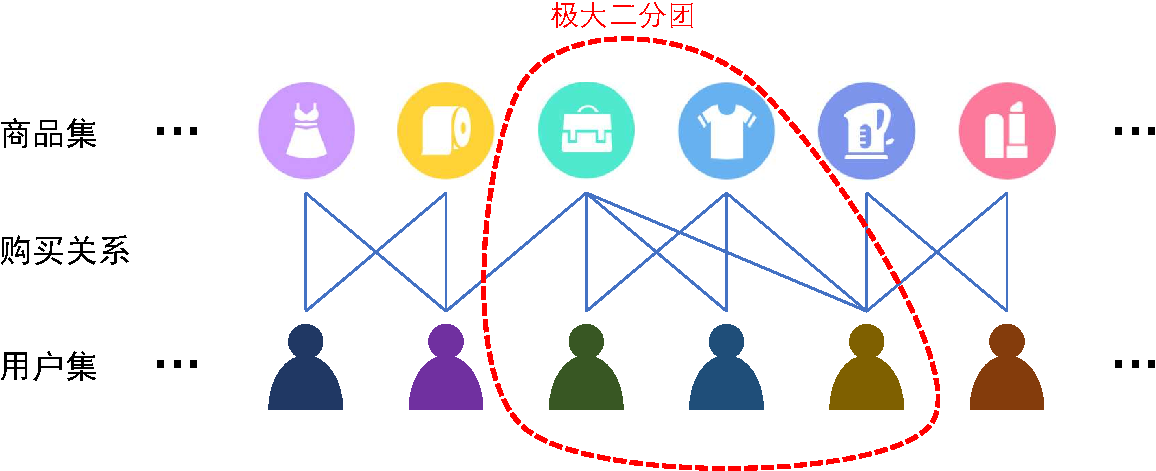
\includegraphics[width=0.7\linewidth]{eg_intro}
  \vspace{0.05in}
  \caption{电子商务场景下的二分图与极大二分团}
  \label{fig:eg_intro}
\end{figure}



% 极大二分团枚举在二分图\textbf{数据挖掘}方面起到重要辅助作用,具有广泛的应用价值。
\textbf{极大二分团枚举在数据挖掘领域具有广泛的应用价值。} (1) 在电子商务场景下,极大二分团被广泛应用于描述用户群体对同一组商品的批量购买行为。电子商务领域的领军企业如阿里巴巴、eBay和亚马逊通常使用二分图表示"用户----购买----商品"的交易关系~\cite{MEB20}。一些不法商家会利用刷单手段,雇佣一批用户购买目标商品,以提高其曝光率并扰乱市场秩序。考虑到极大二分团能有效描绘此类刷单行为,电子商务企业可以通过枚举极大二分团来发现所有可疑交易,提升对刷单行为的检测率~\cite{clickfarm21,MEB20,MEB22,skylinechinese23}。(2) 在社交网络场景下,极大二分团最大程度地描述了用户群体的相同兴趣爱好。通过极大二分团枚举,可以更好地辅助社交推荐系统。通过发现用户之间紧密的连接关系,系统可以推荐给用户其他拥有相似兴趣爱好的用户,从而增加社交互动和用户满意度。同时,极大二分团的枚举还能帮助社交网络平台理解用户行为和需求,进一步优化用户体验,提高平台的粘性和竞争力~\cite{minel06,MBEchinese17}。同时,通过极大二分团的枚举,还有助于对社交网络进行全面分析,有助于发现社交网络中存在的异常风险信息,提升社交网络安全防护工作的能力~\cite{dangerous19,dangerous05}。(3) 在基因分析场景下,极大二分团描述了同一组基因对同一组性状的决定作用。枚举极大二分团能够更好地帮助生物学家理解基因与性状之间的关系。通过分析不同基因之间的连接模式,可以揭示基因之间的相互作用以及它们对性状表现的综合影响。这种基于极大二分团的分析方法能够提供更全面和深入的基因功能研究视角,帮助科学家进一步进行蛋白质-蛋白质相互作用网络分析~\cite{protein11}、从事务数据库中提取基因表型信息~\cite{gene11}、构建最优进化树~\cite{tree04}以及探索基因表达机制~\cite{geneexp11}。此外,极大二分团的枚举还有助于准确预测基因变异对性状造成的影响,并为疾病研究、遗传工程等领域提供重要的指导意义~\cite{gene22,iMBEA14,protein21}。(4)在图神经网络 (Graph Neural Network, GNN) 领域,极大二分团能够辅助对多个节点数据进行打包,从而加速GNN信息聚合。通过识别和利用极大二分团结构,可以将具有相似特征或者相互关联的节点分为同一个二分团,更高效地进行信息传递和计算,提升图神经网络的训练和推理性能~\cite{Pqbiclique21,Pqbiclique23,Pq23}。总而言之,极大二分团的枚举在电子商务、社交网络、基因分析以及图神经网络等领域都发挥着重要的作用。它能够帮助揭示群体行为、发现异常的交易行为、辅助推荐系统和加速信息聚合等任务,为相关领域的研究和实践提供有力支持。

\begin{figure} [t]
  \centering
  \vspace{0.1in}
  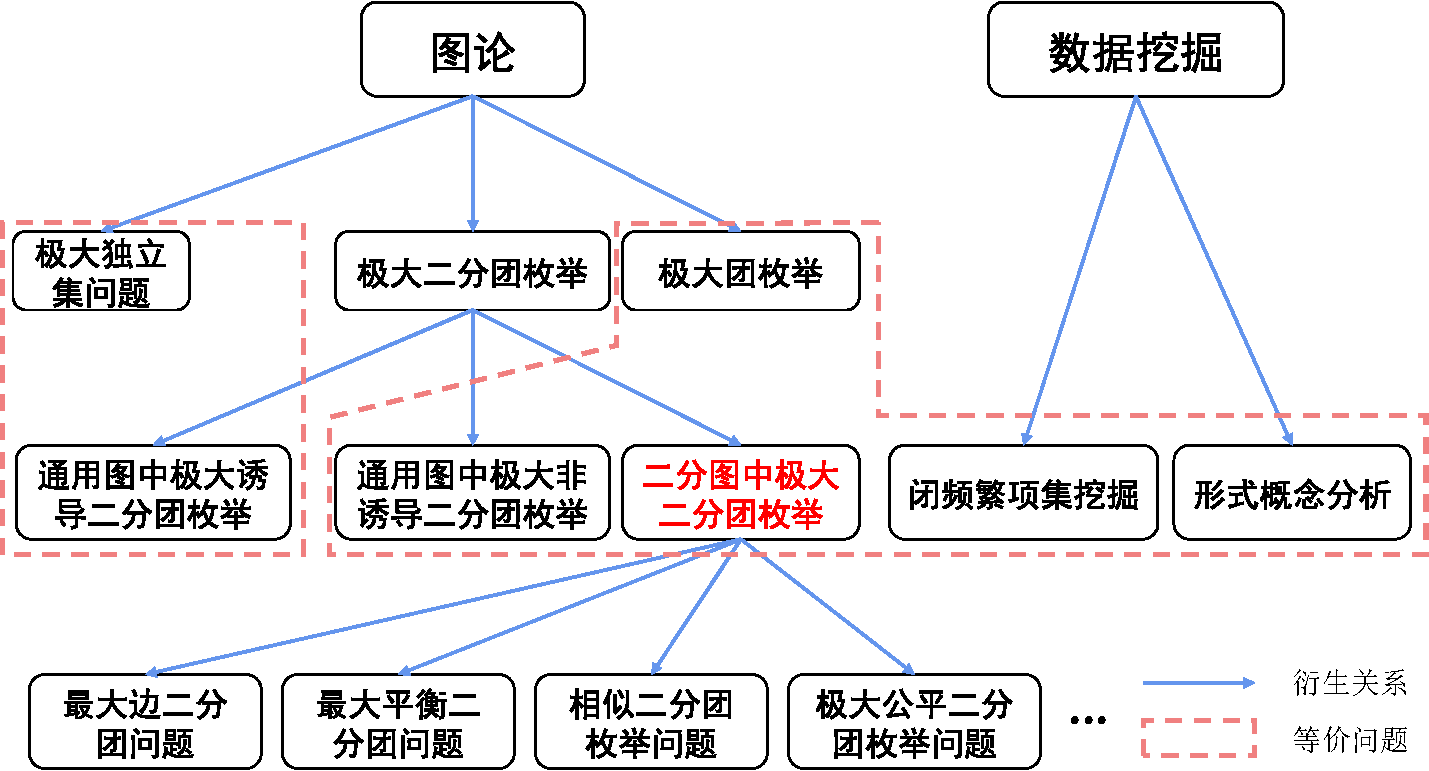
\includegraphics[width=0.9\linewidth]{directory}
  \vspace{0.1in}
  \caption{二分图中极大二分团枚举问题与相关问题的关系图}
  \label{fig:directory}
\end{figure}

\textbf{同时,极大二分团枚举也是图论中的一类经典组合优化问题。}
% 同时,二分图中的极大二分团枚举问题作为\textbf{图论}中的经典组合优化问题,吸引了广泛的研究兴趣。
下面,我们结合图~\ref{fig:directory},从三个方面(相近问题、等价问题和衍生问题)介绍本研究问题与其他相关问题的联系。(1)相近问题:极大二分团是一种特殊的子图,在通用图中同样存在。通用图中的极大诱导二分团枚举问题可转化为极大独立集问题进行求解~\cite{MBE-induced21};通用图中的极大非诱导二分团枚举问题可转化为二分图中的极大二分团枚举问题进行求解~\cite{Proof09}。考虑到二分图中的极大二分团枚举问题具有广泛的应用价值,本文仅研究二分图中的极大二分团枚举问题。(2)等价问题:二分图中的极大二分团枚举问题与许多图论领域和数据挖掘领域的经典问题存在一一映射关系。例如,极大团枚举问题~\cite{MCEchinese17,MCE20,MCEchinese20,MCE-GPU21,MCEchinese21,MCE22,MCEreview22} (Maximal Clique Enumeration, MCE)、闭频繁项集挖掘问题~\cite{FCIM98,FCIM22} (Frequent Closed Itemset Mining, FCIM) 和形式概念分析问题~\cite{FCA21,FCA22} (Formal Concept Analysis, FCA)。很多现有的极大二分团枚举方法都受益于这些相关问题的优化思路,部分相关工作将极大二分团枚举问题规约到这些相关问题进行求解。我们将在第~\ref{sec:related}节详细介绍这些方法。相应地,对二分图中极大二分团枚举问题的优化研究间接地为解决这些问题提供了思路。(3)衍生问题:随着二分图中极大二分团问题研究的深入,近年来,极大二分团枚举方法被应用于最大边二分团搜索~\cite{MEB20,MEB22} (Maximum Edge Biclique Search, MEB) 和最大平衡二分团搜索~\cite{MBB21} (Maximum Balanced Biclique Search, MBB) 等问题中,并衍生出相似二分团枚举问题~\cite{SimilarMBE22}、(p,q)二分团枚举问题\cite{Pqbiclique21,Pqbiclique23,Pq23,pqchinese22}、公平极大二分团枚举问题~\cite{FairMBE23}和二分团渗透社区~\cite{BicliqueCommunity23}等相关问题。一些研究将衍生问题推广到不确定图~\cite{MBEU23}、带符号图~\cite{Sun22,Sun23}、带权重图~\cite{WeightMEB22,WeightMBB22}和动态图~\cite{Ma22}的场景中。
这些衍生问题都基于极大二分团枚举算法,针对各自目标二分团设计特定的剪枝与优化方法,为进一步扩展和拓展极大二分团的应用领域提供了可能性。总之,二分图中极大二分团枚举问题在图论研究中占据重要地位。深入研究该问题将对其他相关问题的研究产生辐射带动作用。


\textbf{然而,大规模二分图中极大二分团枚举问题面临着严峻的挑战。}具体而言,这些挑战主要表现在以下三个方面。(1)搜索空间大。极大二分团枚举问题是一个NP-hard问题,随着二分图规模的增大,其搜索空间呈现出指数级增长的趋势~\cite{MICA04}。然而,在大数据时代的背景下,二分图的规模不断膨胀。以电子商务为例,根据中国商务部的电子商务报告~\cite{ECommerceReport},2022年全国电子商务交易额达到43.83万亿元,与上一年相比增长了3.5\%。此外,仅在2020年,阿里巴巴企业单日的交易次数已超过1亿次~\cite{MEB20}。不断增长的二分图规模使得极大二分团枚举问题的搜索空间进一步加大。(2)计算不规则。与其他图计算问题相似,极大二分团枚举问题主要涉及集合运算。然而,真实世界中的二分图存在着不规则性~\cite{Irregularity12},即每个顶点的邻居数量存在较大的差异,符合幂律分布的特征。这意味着只有少数顶点具有大量的邻居连接,而大多数顶点的邻居数量相对较小。因此,每次集合运算所涉及的顶点数量也各不相同。目前的方法忽视了集合运算的不规则性,导致设计出的枚举方法无法充分发挥其潜力。(3)负载不均匀。主流的极大二分团枚举方法依赖于集合枚举树的实现~\cite{minel06,iMBEA14,PMBE20,ooMBE22}。为了进一步提升枚举速度,研究者们尝试在分布式系统或多核系统中设计并行的极大二分团枚举算法~\cite{mapreduceMBE16,parMBE19}。具体做法是将枚举树拆解成多个子枚举树,并利用充足的计算资源并行处理这些子枚举树。然而,与其他图计算问题不同的是,每个极大二分团所包含的顶点数量是不确定的,这导致子枚举树的高度无法确定,进而增加子了枚举树之间的负载差异,加大了并行扩展的难度。


% 主流的极大二分团枚举方法依赖于集合枚举树的实现。然而与其他图枚举问题不同的是,极大二分团中包含的顶点数量是不固定的,从而导致枚举树的高度也是不固定的。此外,顶点邻居数量呈现幂律分布的特征,进一步增加了枚举树之间的负载差异。若想以并行方式处理多棵子枚举树,每棵子枚举树对应的负载差异增加了并行扩展的难度。


% 首先,极大二分团枚举问题是一种NP-hard问题,即在多项式时间内无法高效地解决。随着二分图顶点数量的增加,极大二分团问题的求解难度呈指数级增长~\cite{MICA04}。这意味着在大规模二分图中进行极大二分团枚举的计算复杂度非常高。举个例子,具有18万个顶点和44万条边的二分图Github中,其内部极大二分团的数量已经超过了5534万个~\cite{konect}。据统计数据显示,目前最优的极大二分团枚举算法ooMBEA~\cite{ooMBE22}。在Github数据集上执行极大二分团枚举任务时,产生的无效枚举数量是极大二分团数量的26倍,这表明仍然存在巨大的优化空间。其次,在大数据时代,二分图的规模仍在不断增加。以电子商务为例,根据中国商务部的电子商务报告~\cite{ECommerceReport},2022年全国电子商务交易额达到43.83万亿元。按可比口径计算,与上一年相比增长了3.5\%。据统计,仅在2020年,阿里巴巴企业一天内的交易次数已超过1亿次~\cite{MEB20}。因此,在这种情况下,如何设计高效的极大二分团枚举算法,并快速地在大规模二分图中找到所需的极大二分团,面临着极大的挑战。最后,相较于其他子图枚举问题,极大二分团枚举问题的特点之一是每个极大二分团的顶点数量较多且不固定,导致该问题更加复杂和不规则~\cite{Irregularity12}。在图枚举算法中,每个被枚举子图的计算时间与子图内顶点数量呈正相关关系,因此极大二分团枚举问题中每个极大二分团的顶点数量差异会导致计算时长上的差异。特别是当枚举涉及到包含许多顶点的极大二分团时,其计算所需时间会显著增加,从而进一步加剧了负载不均衡的问题,严重影响了并行性能。为了提高极大二分团枚举算法的效率和可扩展性,我们需要探索新的方法和技术来解决这些挑战。

综上所述,二分图中的极大二分团枚举问题在电子商务中的虚假交易检测、社交网络推荐、生物医学中的基因分析等热门场景中有着广泛的应用。同时在图论领域扮演着基础问题的关键角色,并在近年来衍生出许多相关问题,成为学术研究热点。然而,在处理大规模二分图时,极大二分团枚举算法面临着挑战,包括搜索空间巨大、计算不规则以及负载分布不均等难题。因此,极大二分团问题受到工业界和学术界的广泛关注。


% 因此,探索在大规模二分图中高效解决极大二分团枚举问题的方法成为一项重要的研究课题。
% 在搜索空间、数据结构以及并行扩展等方面仍存在很大的优化空间。因此,探索在大规模二分图中高效解决极大二分团枚举问题的方法成为一项重要的研究课题。

\section{研究问题}
\label{sec:topic}

本节详细介绍了本文的研究问题,包括对二分图中极大二分团枚举问题的形式化定义,以及该问题的基本求解方法。

\subsection{问题定义}


在问题定义之前,我们首先介绍图论领域的一些基础概念,并提供了随后频繁使用的符号及其含义,如表~\ref{tab:definition}所示。

\begin{longtable}[htbp]{|c|p{12cm}|}
    \caption{本文使用的符号及含义}
    \label{tab:definition} \\
    
    \hline
    符号 & 含义 \\ \hline
    \endfirsthead
    
    \hline
    符号 & 含义 \\ \hline
    \endhead
    
    \hline
    \multicolumn{2}{r}{续下页} \\
    \endfoot
    
    \hline
    \endlastfoot
    
    $G(U,V,E)$ & 一个无向二分图 $G$,其中 $U$ 和 $V$ 是两个不相交的顶点集合,$E$ 是二分图的边集合且 $E \subseteq U \times V$。 \\ \hline
    $u,v$ & 表示二分图 $G$ 中的顶点。其中顶点 $u$ 属于集合 $U$,顶点 $v$ 属于集合 $V$。 \\ \hline
    $N(v)$ & 表示顶点 $v$ 的邻居顶点集合,即 $N(v) = \{u \,|\, (u,v) \in E\}$。 \\ \hline
    $N_2(v)$ & 表示顶点 $v$ 的二跳邻居顶点集合,即 $N_2(v) = \bigcup_{u \in N(v)} N(u) - \{v\}$。 \\ \hline
    $\Delta(v)$ & 表示顶点 $v$ 的度数,即 $\Delta(v) = |N(v)|$。 \\ \hline
    $\Gamma(X)$ & 表示顶点集 $X$ 内顶点的共同邻居,即 $\Gamma(X) = \bigcap_{v \in X} N(v)$。 \\ \hline
    $\Upsilon(X)$ & 表示顶点集 $X$ 内顶点的合并邻居,即 $\Upsilon(X) = \bigcup_{v \in X} N(v)$。 \\ \hline
    $\Delta(X)$ & 表示顶点集 $X$ 内顶点的最大度数,即 $\Delta(X) = \max_{u \in X} |N(u)|$。 \\ \hline
    $\Delta_2(X)$ & 表示顶点集 $X$ 内顶点的最大二跳度数,即 $\Delta_2(X) = \max_{u \in X} |N_2(u)|$。 \\ \hline
    $X_v^+, X_v^-$ & 表示顶点集 $X$ 根据顶点 $v$ 划分成的两个子集。给定一个顶点顺序,$X_v^+$ 包含所有顶点比 $v$ 更大的顶点(顺序在 $v$ 之后的顶点),即顶点$v$的尾部顶点;$X_v^-$ 包含包括 $v$ 顶点在内的所有顶点比 $v$ 更小的顶点(顺序在 $v$ 之前的顶点),即顶点$v$的头部顶点。 \\ \hline
    $L,R,C$ & $L$, $R$ 和 $C$ 指三个两两不相交的顶点集,其中 $L$ 是集合 $U$ 的子集,$R$ 和 $C$ 是集合$V$ 的子集。$L,R$ 和 $C$ 共同构成一个枚举树节点,其中 $(L,R)$ 表示枚举树节点对应的二分团,$C$ 表示用于生成新枚举树节点的候选顶点。对于二分团 $(L,R)$,$L$ 和 $R$ 分别表示二分团的左部顶点集和右部顶点集。 \\ \hline
    $N_L(v)$ & 表示顶点 $v$ 的局部邻居。对于对应二分团 $(L,R)$ 的枚举树节点,$N_L(v) = L \cap N(v)$。 \\ \hline
    $\vec{v}$ & 对于一个枚举树节点,$\vec{v}$ 表示用于生成该枚举树节点的候选顶点,即枚举树中从父节点到子节点的边上的遍历候选顶点。 \\ \hline
    $\alpha, \delta, \beta$ & 对于一棵极大二分团枚举树,$\alpha$ 表示枚举树中产生的极大二分团的数量,$\delta$ 表示枚举树中产生的其他二分团的数量,$\beta$ 表示枚举树中二分团的总数量。可知 $\beta = \alpha + \delta$。 \\ \hline
\end{longtable}

  二分图中的极大二分团枚举问题是在一个无向无权二分图$G(U,V,E)$中的特定的图挖掘问题。随后,我们定义二分图、二分团、极大二分团以及极大二分团枚举问题。

  \begin{definition}
    \textbf{(二分图)} 二分图(Bipartite graph)$G(U,V,E)$ 是一种特殊的图结构,包含两个不相交的顶点集合$U$和$V$,以及连接这些顶点的边集合$E$。在二分图中,边集$E$中的每条边连接的两个顶点分属于不同的顶点集合,即$E \subseteq U \times V$。
    % 是二分图$G(U,V,E)$中的稠密二分子图$(L,R,E')$。其中$L\subseteq U$, $R\subseteq V$, $E' = L \times R \subseteq E$。为了方便,下文中我们直接用顶点集对$(L,R)$表示二分团。
  \end{definition}



\begin{definition}
  \textbf{(二分团)} 二分团(Biclique)是二分图$G(U,V,E)$中的稠密二分子图$(L,R,E')$。其中$L\subseteq U$, $R\subseteq V$, $E' = L \times R \subseteq E$。为了方便,下文中我们直接用顶点集对$(L,R)$表示二分团。
\end{definition}

\begin{definition}
  \textbf{(极大二分团)} 极大二分团(Maximal Biclique)是二分图$G$中的一个二分团,且该二分团不能再添加其他顶点使其成为更大的二分团。
  \label{def:mb}
\end{definition}

\begin{definition}
  \textbf{(极大二分团枚举问题)} 极大二分团枚举问题(Maximal Biclique Enumeration, MBE)的目标是无重复、无遗漏地枚举二分图中的全部极大二分团。
\end{definition}

\begin{figure} [ht]
  % \vspace{0.2 in}
  \centering
  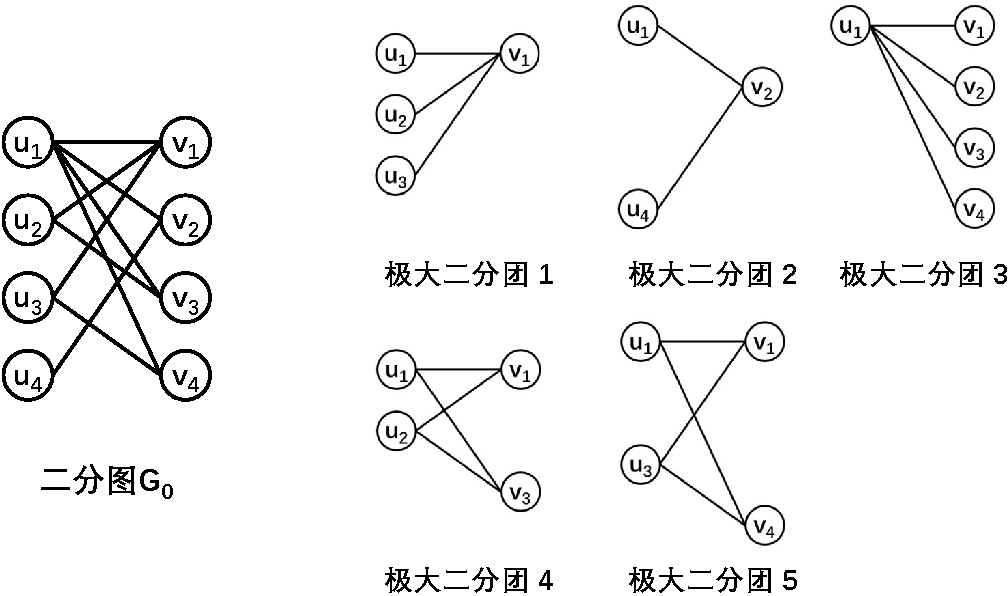
\includegraphics[width=0.7\linewidth]{eg_definition}
  \vspace{0.1 in}
  \caption{二分图中的极大二分团枚举问题示例}
  \label{fig:eg_definition}
\end{figure}

\begin{example}
  图~\ref{fig:eg_definition}给出了一个二分图中的极大二分团枚举问题的示例。其中左图是一个具有8个顶点,9条边的二分图$G_0$,右图展示了二分图中的全部极大二分团,共5个。极大二分团枚举问题即无重复、无遗漏地枚举二分图$G_0$中的全部5个极大二分团。
  
\end{example}

考虑到现有方法在处理大规模二分图时效率低下,本研究从\emph{剪枝能力} 、 \emph{数据结构} 和 \emph{并行实现}等方面入手,探索\textbf{在大规模二分图场景下的高效极大二分团枚举方法}。



% 探索在大规模二分图中高效解决极大二分团枚举问题的方法成为一项重要的研究课题。


\subsection{基本求解方法}
\label{subsec:baseline}
  
  在本节中,我们详细描述了主流的基于集合枚举树的极大二分团问题基本求解方法。我们首先介绍了极大二分团问题中的集合枚举树的定义,接着给出了基于该集合枚举树的极大二分团枚举基本算法,最后分析了该算法的复杂度。

\subsubsection{集合枚举树介绍}
\label{subsec:se}

\begin{figure} [ht]
  % \vspace{0.1 in}
  \centering
  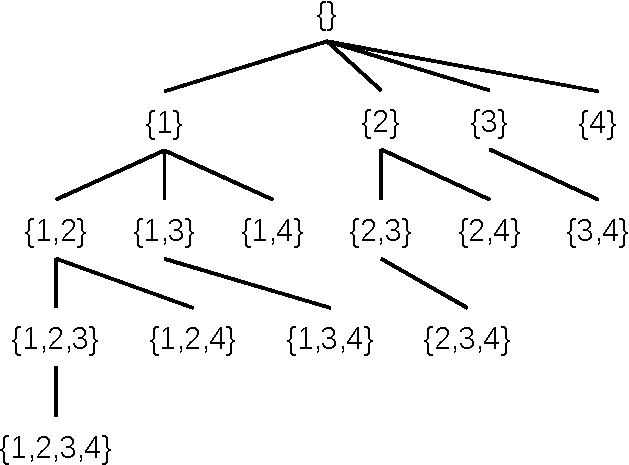
\includegraphics[width=0.45\linewidth]{se_naive}
  \vspace{0.1 in}
  \caption{对于集合$P\{1,2,3,4\}$的集合枚举树}
  \label{fig:se_naive}
\end{figure}


\textbf{集合枚举树}(Set Enumeration Tree, SE tree)是一种用于有序地枚举特定集合全部子集的数据结构,即枚举该集合的幂集~\cite{SEtree92}。它为解决搜索空间为特定集合幂集的子集的问题提供了一种完整且无冗余的搜索技术。具体而言,集合枚举树如图~\ref{fig:se_naive} 所示,根节点表示空集,每个节点对应一个子集,其子节点代表在该子集基础上添加一个新元素所得到的子集。对于二分图中的极大二分团枚举问题而言,每个二分团的集合$R$即为二分图中集合$V$的一个独特子集。因此,通过引入集合枚举树可以无重复、无遗漏地枚举全部可能的极大二分团,进而有效地求解极大二分团枚举问题。

对于应用于极大二分团枚举问题的集合枚举树,我们从以下三个角度对其进行了规范化描述:

\begin{itemize}
  \item 节点结构:每个树节点为一个三元组$(L,R,C)$。在一个二分图$G(U,V,E)$,集合$L$是集合$U$的子集,集合$R$和集合$C$是集合$V$的两个不相交子集。集合$L$和$R$构成一个二分团,其中集合$L$包含左部顶点,集合$R$包含右部顶点。集合$C$包含用于扩展集合$R$的候选顶点。
  \item 节点生成:枚举树从根节点$(U,\emptyset,V)$ 开始遍历。对于当前节点$(L,R,C)$,枚举树按顺序访问集合$C$中的每个候选顶点$v'$以生成一个新的节点$(L',R',C')$。集合$L'$包含集合$L$和集合$N(v')$中的共同顶点。集合$R'$包含集合$R$中的顶点、顶点$v'$以及集合$C$中与集合$L'$内顶点均相连且未被访问的顶点。集合$C'$包含集合$C$中与集合$L'$内顶点部分相连的且未被访问的顶点。
  \item 节点检查:当且仅当集合$L'$的共同邻居等于集合$R'$, 即$\Gamma(L')=R'$时,节点$(L',R',C')$通过节点检查,输出一个极大二分团。
\end{itemize}

此外,一些研究~\cite{iMBEA14,ooMBE22}在每个枚举节点中额外引入集合$Q$作为辅助节点检查的工具,构成四元组$(L,R,C,Q)$。其中集合$Q$于存储已访问的候选顶点,以帮助检查节点是否对应非极大二分团。具体而言,当集合$Q$中存在任意一个顶点$v_q$,并且它的邻居包含了集合$L$中的所有顶点时,根据定义~\ref{def:mb}我们可以推断当前节点对应的二分团$(L,R)$可以添加顶点$v_q$构成新的二分团,即$(L, R\cup\{v_q\})$,从而我们可以判定当前节点对应一个非极大二分团。然而,使用集合$Q$需要额外的存储和计算开销。幸运的是,我们观察到可以通过访问$L$中的任意顶点$u_l$的邻居$N(u_l)$来高效地替代集合$Q$的作用。具体而言,当集合$N(u_l)$中存在一个不在$R$集合中的顶点$v^*$,并且它的邻居包含了集合$L$中的所有顶点时,我们可以推断当前节点对应的二分团$(L,R)$可以添加顶点$v^*$构成新的二分团,从而判定当前节点对应一个非极大二分团。因此,在枚举树的介绍和相关算法中,我们不再引入集合$Q$。

\subsubsection{基于集合枚举树的极大二分团枚举基本算法}
\label{subsec:algorithm}
  结合上一节对集合枚举树的定义与描述,我们给出了基于集合枚举树的极大二分团枚举基本算法。

\begin{algorithm}[H]
    \begin{algorithmic}[1]
        \normalsize
        \REQUIRE 二分图 $G(U,V,E)$
        \ENSURE 所有极大二分团
        
        \renewcommand{\algorithmicwhile}{\textbf{procedure}}
        \renewcommand{\algorithmicdo}{\textbf{:}}


        \STATE \textsf{biclique\_search\_basic}$(U,\emptyset,V)$;
        \WHILE{\textsf{biclique\_search\_basic}$(L,R,C)$}
        \renewcommand{\algorithmicdo}{\textbf{do}}
          \FOR{$v' \in C$}
            \STATE $L' \leftarrow L \cap N(v')$; $R'\leftarrow R$; $C' \leftarrow \emptyset$;
            \FOR{$v_c \in C$}
              \IF{$L' \cap N(v_c) = L'$}
                \STATE $R' \leftarrow R' \cup \{v_c\}$;
              \ELSIF{$L' \cap N(v_c) \neq \emptyset$}
                \STATE $C' \leftarrow C' \cup \{v_c\}$;
              \ENDIF
            \ENDFOR
            \IF{$\Gamma(L') = R'$}
              \STATE 输出极大二分团$(L', R')$;
              \STATE \textsf{biclique\_search\_basic}$(L',R',C')$;
            \ENDIF
            \STATE $C \leftarrow C \setminus \{v'\}; $
          \ENDFOR

        \ENDWHILE

    \end{algorithmic}
    \caption{基于集合枚举树的极大二分团枚举算法}
    \label{alg:se_mbe}
\end{algorithm}

算法~\ref{alg:se_mbe}总结了基于集合枚举树的极大二分团枚举算法的基本枚举过程。具体而言,该算法从根节点$(U,\emptyset,V)$开始,递归地调用\textsf{biclique\_search\_basic}过程 (第1行)。过程\textsf{biclique\_search\_basic}接收一个枚举树节点作为输入,即该节点对应的集合$L$,$R$和$C$ (第2行)。在处理当前枚举节点时,该过程会逐个遍历$C$中的顶点$v'$ (第3行),然后根据集合枚举树的节点生成规则生成新节点$(L',R',C')$ (第4-11行)。随后,过程按照节点检查规则对新生成的节点$(L',R',C')$进行检查 (第12行)。如果该节点对应一个极大二分团,则输出该二分团 (第13行),并递归地调用过程\textsf{biclique\_search\_basic}以节点$(L',R',C')$为根节点继续探索子枚举树 (第14行);否则,我们知道该节点对应非极大二分团,跳过该节点。为保证$C$中的顶点都未被访问,过程会及时从$C$中移除已访问的顶点$v'$ (第16行)。我们用下面的例子对该算法进行说明。


\begin{figure} [ht]
  \vspace{0.1 in}
  \centering
  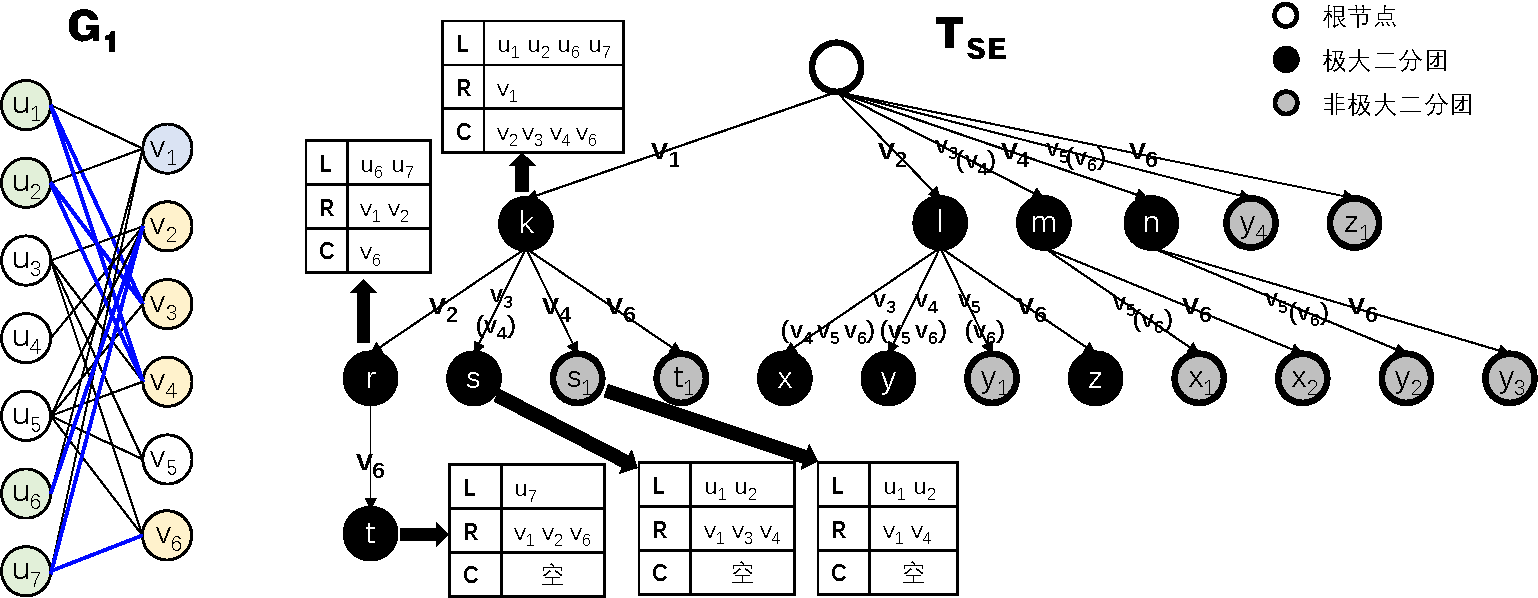
\includegraphics[width=0.98\linewidth]{se_mbea}
  \vspace{0.1 in}
  \caption{算法~\ref{alg:se_mbe}在二分图$G_1$上的集合枚举树}
  \label{fig:se_mbea}
\end{figure}

\begin{example}
  \label{example:se}
  图~\ref{fig:se_mbea}展示了算法~\ref{alg:se_mbe}在二分图$G_1$上的集合枚举树$T_{SE}$。
  \footnote{为了方便比较,全文中具有相同字母标识的节点在枚举树中共享相同的集合$L$,只有没有下标的节点会输出极大二分团。例如,节点$s$和节点$s_1$具有相同的集合$L$,但只有节点$s$会输出一个极大二分团。我们使用集合的下标来表示该集合隶属于哪个节点。例如$L_s$表示节点$s$的集合$L$。 
}
我们从根节点开始,通过深度优先搜索逐个遍历候选顶点,递归地搜索子空间。首先,我们通过遍历顶点$v_1$生成节点$k$。按照算法~\ref{alg:se_mbe}中第4-11行的计算方法,我们可以计算得到$L_k=N(v_1)=\{u_1, u_2, u_6, u_7\}$,$R_k=\{v_1\}$,$C_k=\{v_2,v_3,v_4,v_6\}$。根据节点检查规则,因为$\Gamma(L_{k}) = \{v_1\} = R_{k}$,所以节点$k$输出一个极大二分团并继续探索以节点$k$为根节点的子枚举树。为便于观察,我们在图$G_1$中标记了节点$k$中的顶点,即$L_k$,$R_k$和$C_k$中的全部顶点,并标出了集合$L_k$与集合$C_k$之间的边。

接下来,节点$k$遍历顶点$v_2$生成节点$r$。同理,我们可以计算得到$L_{r} = N(v_2) \cap L_{k} 
= \{u_3, u_4, u_5, u_6, u_7\} \cap \{u_1, u_2, u_6, u_7\} = \{u_6, u_7\}$, $R_{r} = R_{k} \cup (C_{k} \cap \Gamma(L_{r})) = \{v_1\} \cup (\{v_2, v_3, v_4, v_5\} \cap \{v_1, v_2\}) = \{v_1, v_2\}$。集合$C_{r}$中仅包含顶点 $v_6$,因为顶点$v_3$, $v_4$和 $v_5$不与集合$L$中的任何顶点相连。

继续这个过程,我们可以计算得到节点$s$以及节点$s_1$。节点$s$对应二分团$(\{u_1, u_2\},$ $\{v_1, v_3, v_4\})$,节点$s_1$对应二分团 $(\{u_1, u_2\}, \{v_1, v_4\})$。根据节点检查规则,因为$\Gamma(L_{s_1}) = \{v_1, v_3, v_4\} \neq R_{s_1} = \{v_1, v_4\}$,所以节点$s_1$对应一个非极大二分团。具体地,与节点$s$相比,节点$s_1$不能用$v_3$来扩展该节点中的集合$R_{s_1}$。这是因为在生成节点$s_1$时,根据深度优先搜索的规则,顶点$v_3$已被访问并用于生成节点$s$。因此,在节点检查之后,我们删除了节点$s_1$。同理,其他节点可以类似地生成。

\end{example}

在算法~\ref{alg:se_mbe}的基础上,现有的基于枚举树的极大二分团枚举算法的优化方法主要包括改变节点候选顶点的遍历顺序~\cite{minel06,iMBEA14,PMBE20,ooMBE22}、设计剪枝方法以提前裁剪产生非极大二分团的节点~\cite{iMBEA14,PMBE20,ooMBE22},以及并行优化~\cite{mapreduceMBE16,parMBE19}。在~\ref{sec:opt}节中,我们将对上述优化方法进行详细说明,并介绍它们在实际应用中的效果。

\subsubsection{算法复杂度分析}
\label{subsec:baseline_analysis}

结合算法伪代码,我们从时间复杂度和空间复杂度两个方面对算法~\ref{alg:se_mbe}进行分析。

\textbf{时间复杂度:} 我们首先分析枚举树中每个节点的计算时间,随后分析枚举树中的枚举节点数量,最终得到算法~\ref{alg:se_mbe}的时间复杂度。平均而言,对于每个节点$(L',R',C')$的计算包括节点生成(第4-11行)和节点检查(第12行)两个部分。由于集合$C$中最多包含$|V|$个顶点,且每个顶点的集合交集运算需要$O(\Delta(V))$的时间,因此节点生成过程的时间复杂度为$O(|V|\Delta(V))$。而节点检查过程中,我们可以通过只访问二分图中的每条边一次来获取$\Gamma(L')$的值,因此节点检查的时间复杂度为$O(|E|)$(或$O(|V|\Delta_{avg}(V))$)。综上,每个节点的计算时间为$O(|V|\Delta(V))$。为了量化算法的计算时间,我们用$\beta$来表示枚举树中节点的数量。最终,算法的时间复杂度为$O(|V|\Delta(V)\beta)$。

\textbf{空间复杂度:} 由于算法~\ref{alg:se_mbe}按照深度优先的方式进行搜索,我们可以对枚举树中每个节点占用的空间进行分析,并结合枚举树的高度以及输入二分图所占用的空间,得到算法的空间复杂度。对于每个节点$(L',R',C')$,集合$L'$最多包含$\Delta(V)$个顶点,集合$R'$和$C'$最多包含$|V|$个顶点。在二分图中,集合$V$内顶点的数量通常远高于任何单个顶点的度数,因此每个节点的空间开销为$O(\Delta(V)+|V|)=O(|V|)$。在递归过程中,节点的集合$L$内的顶点数量不断减少,因此我们可以确定枚举树的高度为$O(\Delta(V))$。考虑到二分图$G(U,V,E)$需要占用$O(|U|+|V|+|E|)=O(|E|)$的空间,最终算法的空间复杂度为$O(|E|+|V|\Delta(V))$。




\section{国内外研究现状}
\label{sec:related}

作为图论中的基础问题,关于极大二分团枚举问题的研究最早可追溯到1962年~\cite{MBE62}。在过去的几十年中,国内外学者对二分图中的极大二分团枚举问题进行了深入的研究,并取得了一系列重要的成果。

\begin{figure} [H]
  \centering
  \vspace{0.2in}
  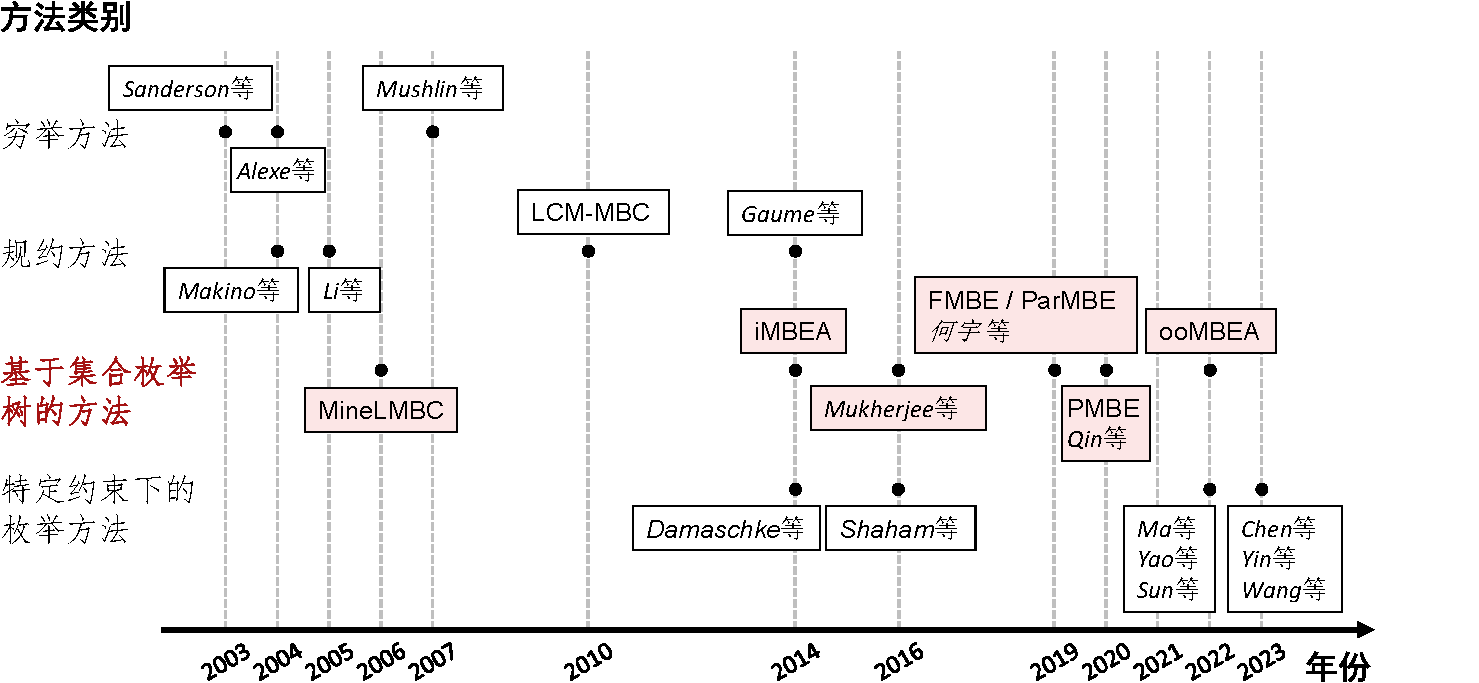
\includegraphics[width=0.98\linewidth]{related_work}
  \vspace{0.1in}
  \caption{极大二分团枚举领域国内外研究情况梳理}
  \label{fig:related_work}
\end{figure}

我们在图~\ref{fig:related_work}中对国内外相关研究进行了梳理和总结,将其分为四类。早期的研究主要采用穷举方法和规约方法,而当前的主流工作采用基于集合枚举树的方法。同时,近期的研究涉及到特定约束下的枚举方法。接下来,我们将详细介绍这四类方法。

% 我们在图~\ref{fig:related_work}中梳理并总结了国内外研究现状,将相关研究工作分为四类。早期的研究方法主要包括穷举方法和规约方法,目前的主流极大二分团枚举方法基于集合枚举树的方法实现,同时,近期的相关工作属于变种,开始研究特定约束下的二分团枚举方法,随后,我们对这四类方法进行详细说明。
% 对国内外的研究情况进行了梳理与总结。从图中可以得知,基于集合枚举树的方法目前是解决通用极大二分团枚举问题的主流方法。目前已有的极大二分团枚举方法可以归为以下四个大类:

\subsection{穷举方法}

解决极大二分团枚举问题的一种直观方法是使用穷举法生成并存储所有可能的二分团,然后对这些二分团进行极大性检测。早期工作以此观察为基础,提出了关于极大二分团枚举问题的暴力穷举求解方法。Sanderson等人提出了一种迭代算法,逐步构建出全部可能的二分团~\cite{exhaust03}。具体而言,该算法首先选取二分图中一个顶点集中的单一顶点作为初始二分团。然后,它遍历其他顶点,逐一将其加入到当前的二分团中构成新的二分团,并对所得的新的二分团进行极大性检测。随后,Alexe等人提出了一种共识算法,用于生成极大二分团。该算法将每个顶点及其邻居作为初始候选二分团,并通过不断进行共识分析来扩展新的候选二分团~\cite{MICA04}。在生成的新二分团中,还进行判断以确保其为极大二分团且没有重复。整个过程会持续进行,直到候选二分团集合不再增加。此外,Mushlin等人利用集合扩展操作构建二分团,并利用哈希表进行极大性检测。他们引入了评价指标,以支持在枚举过程中对二分团的优先级进行排序~\cite{exhaust07}。尽管这些方法能够解决极大二分团枚举问题,但它们没有充分考虑搜索空间的剪枝优化,因此在计算过程中不可避免地会产生大量非极大二分团,导致计算和存储开销增加。同时,由于时间复杂度较高,这些方法无法应用于规模较大的二分图上的极大二分团枚举问题的求解。

\subsection{规约方法}

考虑到极大二分团枚举问题和其他问题的联系,学者们尝试将二分图中的极大团枚举问题规约到其他问题,并用其他问题中的已有方法进行求解。(1) 规约到极大团枚举问题。Makino等人观察到二分图上的极大二分团枚举问题可以通过图膨胀的方式映射到通用图上的极大团枚举问题进行求解~\cite{Makino04}。具体而言,他们将二分图中的每个顶点集合内的任意两个顶点添加一条边,从而膨胀原二分图中的每个极大二分团,使其对应于膨胀后通用图中的一个极大团。通过这种方式,二分图上的极大二分团枚举问题可以被等价地转化为通用图上的极大团枚举问题。然而,需要注意的是,尽管通用图上的极大团枚举问题已经在学术界得到广泛研究,并存在一些有效的极大团枚举方法~\cite{MCEparallel20,MCE20,MCE22,MCE-GPU21,MCE-22},但直接应用这些方法并不实用。这是因为图的膨胀会引入大量的新边,从而导致计算难度的增加,并严重影响了计算性能。(2) 规约到闭频繁项集挖掘问题。Zaki等人注意到事务数据库中的闭频繁项集与二分图中的极大二分团存在一一对应的关系~\cite{FCIM98}。基于这个对应关系,Li等人指出了数据挖掘领域中一些经典算法对于极大二分团枚举问题的解决具有帮助作用~\cite{correspondence05},例如FPclose~\cite{fpclose04}和LCM~\cite{lcm04}等算法。通过计算闭频繁项集集,可以得到极大二分团中的一个顶点集合,进而计算另一个顶点集合以构成二分团。Li等人还在LCM算法的基础上提出了LCM-MBC算法来进行极大二分团枚举~\cite{lcmmbc07}。然而,对于闭频繁项集挖掘算法而言,在大规模事务性数据库中将支持度设置为1进行闭频繁项集挖掘是非常困难的~\cite{iMBEA14}。(3)规约到形式概念分析问题。Gaume等人指出二分图中的极大二分团与形式概念分析问题中的形式概念存在平行关系~\cite{fcambe10}。因此,现有的形式概念分析相关的工作~\cite{FCA15,FCA21,FCA22}可以用于极大二分团枚举问题的求解。然而,形式概念分析相关的工作主要在二进制数据上展开~\cite{FCA15},即源数据通过位图方式存储并以位运算的方式开展计算。由于现实中的二分图是稀疏的,位图存储方式会带来大量的内存开销,这导致前沿的形式概念分析算法只能在小图上进行~\cite{FCA21,FCA22},在大规模二分图中会带来内存超过限制的问题。综上所述,规约方法在大规模二分图场景下是低效的。

% \begin{figure} [t]
%   \centering
%   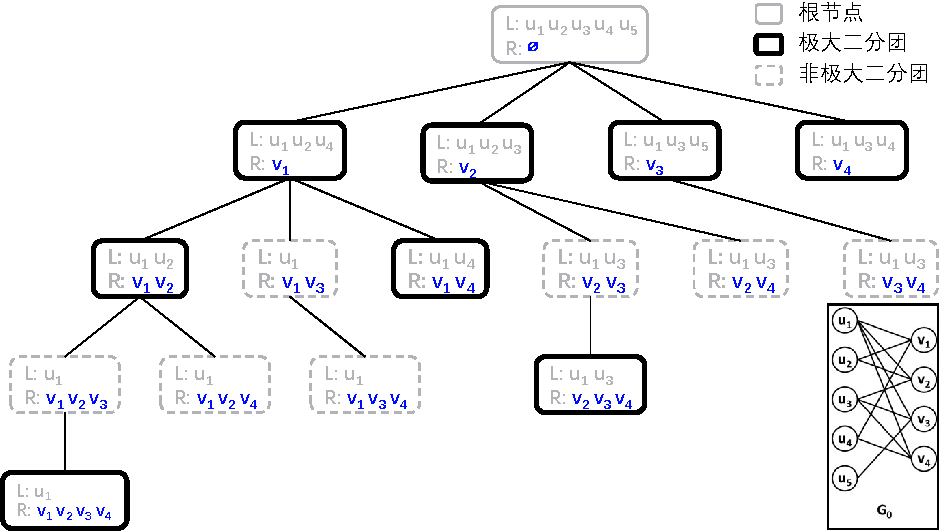
\includegraphics[width=0.62\linewidth]{se_tree}
%   \caption{极大二分团枚举算法中的集合枚举树}
%   \label{fig:se}

% \end{figure}

\subsection{基于集合枚举树的枚举方法}

如~\ref{subsec:baseline}节所述,目前,主流且高效的极大二分团枚举算法基于集合枚举树~\cite{SEtree92}的数据结构实现。
%集合枚举树是一种用于有序地枚举特定集合的所有子集的工具。 给定一个二分图$G(U, V, E)$,其中$U$和$V$表示两个不相交的顶点集合,$E$表示边集合,$E \subseteq U \times V$。该类枚举算法首先利用集合枚举树生成集合$V$的全部子集,然后将每个集合$V$的子集扩展成二分团,并输出其中的全部极大二分团。图~\ref{fig:se}展示了一棵用于极大二分团枚举的集合枚举树。集合枚举树首先将集合$V$的全部子集无重复地生成到每个树节点的集合$R$中(标记为蓝色),然后每个节点将所有与$R$内顶点完全相连的顶点作为顶点的集合$L$,最后枚举其中所有的极大二分团$(L,R)$。
2006年,Liu等人提出MineLMBC算法~\cite{minel06},首次引入集合枚举树,采用分治法求解极大二分团枚举问题。此后,基于枚举树的极大二分团枚举方法得到了不断优化。为了减少搜索空间、提升计算效率,研究者们相继提出了不同的优化技术。Zhang等人提出iMBEA算法~\cite{iMBEA14},采用了顶点度数升序排序和排除顶点集等技术,以减少枚举时间。Das等人提出FMBE算法~\cite{parMBE19},通过主动计算顶点的二跳邻居作为候选顶点集合,加速了枚举过程。Abidi等人提出PMBE算法~\cite{PMBE20},借鉴了极大团枚举问题中的枢纽顶点思路,利用枢纽顶点进行剪枝。Chen等人提出ooMBEA算法~\cite{ooMBE22},引入了单边排序和批量枢纽顶点剪枝等技术,进一步减少了枚举时间。为了进一步提高效率,研究者们设计了并行极大二分团枚举算法。Mukherjee等人利用MapReduce框架实现了分布式极大二分团枚举算法CDFS~\cite{mapreduceMBE16}。然而,大量的跨节点通信开销导致该算法效率较低。Das等人提出多核算法ParMBE~\cite{parMBE19},但该算法的并行性受到计算核心数量的限制。此外,国内的He等人提出优化的sMBEA算法~\cite{MBEHe18,MBEchinese19},Qin等人利用栈的特性实现了EMBE算法~\cite{MBEQin20}。然而,相较于主流算法(如FMBE、PMBE、ooMBEA),这些算法存在较大的性能差距。综上所述,基于枚举树的极大二分团枚举方法
% 适合解决大规模二分图中的极大二分团枚举问题,但
仍存在较大的优化空间。

\subsection{特定约束下的枚举方法}

除了上述研究,一些学者对输入的二分图以及输出的极大二分团进行了特定的约束。Damaschke等人提出了一种输出敏感的极大二分团枚举算法~\cite{Damaschke14},该算法基于二分图中顶点度数的倾斜分布。然而,该算法对输入二分图的要求较为严格,仅适用于特定情况下的求解,无法很好地适用于一般二分图。Shaham等人提出了基于聚类的方法~\cite{Shaham16},在二分团搜索的子空间中利用蒙特卡洛方法获取随机种子并将其扩展为极大二分团。然而,这种方法只能枚举部分的极大二分团,无法覆盖所有可能的极大二分团。针对动态二分图,Ma等人提出了一种有效保持最大二分团性质的框架,该框架可以在动态变化的二分图上进行高效的极大二分团枚举~\cite{Ma22}。此外,近年来的一些研究工作定义了特殊类型的极大二分团,并对这些特殊类型的二分团进行枚举。例如,Yao等人定义了极大相似二分团~\cite{SimilarMBE22},Sun等人定义了极大平衡有符号二分团~\cite{Sun22}和最大有符号二分团~\cite{Sun23},Chen等人用多个极大二分团并集定义了二分团渗透社区~\cite{BicliqueCommunity23},Yin等人定义了极大二分团的公平性~\cite{FairMBE23},而Wang等人定义了不确定图场景下的极大二分团~\cite{MBEU23}。这些算法都基于极大二分团枚举算法,并在枚举过程中对输出进行适当的约束和限制,以适应特定的问题需求。然而,这些算法主要关注特定约束场景下的搜索空间剪枝与优化,难以用于加速传统的极大二分团枚举问题。综上所述,极大二分团枚举在这些研究中发挥着基础性作用。

% 除了上述工作外,其他研究对输入的二分图以及输出的极大二分团进行了特定的约束。Damaschke等人提出了一种输出敏感的极大二分团枚举算法~\cite{Damaschke14},该算法基于二分图中顶点度数的倾斜分布。然而,该算法对输入二分图的要求较为苛刻,只适用于特定情况下的求解,并不能很好地适用于一般二分图。Shaham等人提出基于聚类的方法~\cite{Shaham16},在二分团搜索的子空间中利用蒙特卡洛方法获取随机种子并将其扩展为极大二分团。然而,这种方法只能枚举部分的极大二分团,无法覆盖所有可能的极大二分团。针对动态二分图,Ma等人提出了一种有效保持最大二分团性质的框架,该框架可以在动态变化的二分图上进行高效的极大二分团枚举。另外,近年来的一些研究工作定义了特殊类型的极大二分团,并对这些特殊类型的二分团进行枚举。例如,Yao等人定义了极大相似二分团~\cite{SimilarMBE22},Sun等人定义了极大平衡有符号二分团~\cite{Sun22}和最大有符号二分团~\cite{Sun23},Chen等人用多个极大二分团并集定义了二分团渗透社区~\cite{BicliqueCommunity23},Yin等人定义了极大二分团的公平性~\cite{FairMBE23}以及Wang等人定义了不确定图场景下的极大二分团~\cite{MBEU23}。这些算法都是基于极大二分团枚举算法,并在枚举过程中对输出进行适当的约束和限制,以适应特定的问题需求。然而这些算法只注重在特定约束场景下的搜索空间剪枝与优化,这些方法难以用于加速传统的极大二分团枚举问题。综上所述,极大二分团枚举在这些研究中发挥着基础性作用。


\section{研究挑战}

尽管在极大二分团枚举领域已经有很多出色的工作,但是在处理大规模二分图时,已有方法的计算性能仍然有很大的提升空间。本节将指出主流的基于集合枚举树的枚举方法所面临的三个共性问题,并介绍解决这些问题所面临的具体挑战。

\subsection{搜索空间大,剪枝方法欠佳}

极大二分团枚举问题具有搜索空间大的特点。常见的图算法,如深度优先搜索~\cite{wiki-dfs}、广度优先搜索~\cite{wiki-bfs}、最小生成树~\cite{wiki-mst}、最短路径等算法~\cite{wiki-sssp},其搜索空间随着图的规模线性增长。而常见的图模式挖掘算法的目标子图往往只包含少量顶点~\cite{peregrine20,pangolin20,g2miner22,decomine22,khuzdul23,gamma23,Graphset23},例如三角计数问题中目标子图仅包含3个顶点~\cite{triangle18}。相比之下,极大二分团枚举问题的搜索空间更大,因为它随着二分图中顶点数量的指数级增长,并且目标子图(即极大二分团)中的顶点数量相对较多。为了应对搜索空间巨大的挑战,研究人员提出了各种优化技术,旨在减少搜索空间中产生非极大二分团的无效枚举节点,进而减少枚举时间。然而,由于搜索空间的规模庞大,现有的优化方法往往难以完全覆盖所有无效节点。具体而言,通过~\ref{subsec:ambea_exp_overall}节的实验,我们观察到现有的最新算法ooMBEA在Github数据集上需要检查并消除比极大二分团数量多26倍的产生非极大二分团的无效枚举节点。这些无效枚举节点带来大量的节点检查开销,严重降低了计算性能。因此,如何设计高效的剪枝方法来裁剪巨大搜索空间仍然是一个关键的挑战。


\subsection{计算不规则,单一结构低效}

极大二分团枚举问题具有计算不规则的特点。与其他图计算问题类似,在真实世界中,二分图的顶点邻居数量存在较大差异,导致每次计算涉及的顶点数量不同,即计算不规则~\cite{Irregularity12}。为了高效地解决这类问题,研究者们提出了多种存储结构来表示图的邻接关系。常用的存储结构包括位图~\cite{lcm04,lcmmbc07,FCA15,FCA21,FCA22}、邻接表~\cite{iMBEA14,PMBE20,ooMBE22}和哈希表~\cite{parMBE19}。不同的存储结构适用于不同场景。
例如,位图结构采用位运算,具有高效的计算能力,但在稀疏图场景下会占用更多的存储资源,因此适用于稠密小图;邻接表精确地存储每个顶点的邻居信息,在处理稀疏大图时占用较少的内存,但计算过程需要执行大量的比较运算,其运行时间与顶点个数成正比,会导致计算相对低效,因此适用于稀疏大图;哈希表具有灵活性和便于快速查找的特点,可以快速判断任意两个顶点之间的连接关系,但相比邻接表,它需要更多的存储空间并且访问方式更为随机。然而,目前的研究往往采用固定的数据结构来存储顶点的邻居信息,未能充分发挥不同数据结构的优势。因此,在枚举过程中如何动态选择合适的存储结构,发挥计算潜力,是一个关键挑战。



\subsection{负载不均匀,并行扩展性差}

极大二分团枚举问题具有负载不均匀的特点,限制了问题的并行扩展能力。为了进一步提高问题求解的效率,研究人员尝试设计并行算法来处理极大二分团枚举问题~\cite{mapreduceMBE16, MBEHe18, parMBE19}。这些算法将整个集合枚举树分解成多个子枚举树,然后利用分布式系统或多核CPU的大量计算资源来并行处理这些子树。然而,由于不同子枚举树的极大二分团的大小不同,导致计算负载之间存在较大差异。因此,即使有大量计算资源可用,计算任务的运行时间仍然受限于最耗时的负载。GPU作为一种专门用于并行计算的硬件设备,由于其内部拥有大量的计算单元,非常适合处理并行任务。然而,由于GPU和CPU在体系结构、内存层次结构以及编程模型等方面存在较大差异,现有的极大二分团枚举算法无法直接迁移到GPU系统中。尽管GPU被广泛用于加速相关的图算法,如极大团枚举~\cite{MCEGPUBitset13,MCEGPUdpp17,MCE-GPU21} 和图模式挖掘~\cite{g2miner22,SubgraphGpu22,Kclique22,stmatch22},但在GPU上进行极大二分团枚举问题仍然具有挑战性。具体来说,GPU上的极大二分团枚举问题面临着与极大二分团枚举问题类似的性能问题,许绍显等人指出GPU加速极大团枚举问题的研究极为有限~\cite{MCEreview22}。即使最新的基于GPU的极大团枚举算法GBK~\cite{MCE-GPU21} 获得较低的性能,也仅与CPU上的单线程串行算法相当。GPU上的子图枚举问题中被枚举子图通常仅包含少量顶点,而极大二分团通常包含大量顶点,因此带来更加严重的负载不均问题,导致最新的基于GPU的GPM框架G$^2$Miner~\cite{g2miner22}与GraphSet~\cite{Graphset23}中的优化无法直接解决GPU上进行极大二分团枚举面临的负载不均匀问题。因此,如何实现负载均衡并突破现有算法在并行能力方面的限制,设计基于GPU的并行极大二分团枚举方法是一个重要挑战。

\section{研究内容}



针对上一节提到的三个方面的研究挑战,本文分别从这三个角度对大规模二分图场景下的极大二分团枚举问题进行深入研究,并相应地提出了三个独立高效的算法,相较现有方法均有明显的性能提升。具体研究内容如下:

第一,针对现有剪枝方法效率低下的问题,本文提出了激进的极大二分团枚举算法AMBEA(Aggressive MBE Algorithm)。我们观察到,现有算法为了保证正确性,仅允许使用部分顶点生成新的枚举节点,导致产生大量非极大二分团;同时,现有的剪枝方法总是在节点检查后被动执行,限制了剪枝能力。因此,我们设计了以下两种方法:(1)激进的集合枚举树,允许使用全部顶点生成新的枚举节点,并利用父子节点间的联系消除枚举树中的重复二分团;(2)激进的顶点合并剪枝方法,在枚举节点生成的同时,主动合并具有相同局部邻居的顶点,提升剪枝效率。实验结果显示,AMBEA算法相较于其他次优的现有算法,可以压缩搜索空间9.0倍,并获得最多5.3倍的性能提升。

第二,针对现有静态数据结构低效的问题,本文提出了自适应的极大二分团枚举算法AdaMBE(Adaptive MBE)。我们观察到,现有算法在计算过程中,包含活跃顶点的计算子图在动态变化,导致冗余的内存访问和低效的集合运算性能。因此,我们设计了以下两种方法:(1)基于局部计算子图的优化方法,在该子图上完成节点生成等核心计算操作,减少了在该子图外的冗余顶点访问;(2)基于位图的动态子图方法,在小的计算子图上利用位图加速集合运算。实验结果显示,AdaMBE算法相较于其他次优的现有算法获得了最多49.7倍的性能提升,并成功应用于超过百亿极大二分团的大数据集。

第三,针对现有基于CPU的算法并行扩展性差的问题,本文提出了基于GPU的极大二分团枚举算法GMBE(GPU-based MBE)。我们观察到,将现有算法迁移到GPU上主要面临内存短缺、线程分歧和负载不均三方面问题。因此,我们设计了以下三种方法:(1)基于枚举节点重用的迭代方法,通过重用父节点内存生成子节点,避免为大量子节点动态分配内存;(2)局部邻居数量感知的剪枝方法,通过对局部邻居数量这一中间结果进行批量比较,在剪枝的同时最小化线程分歧问题;(3)负载感知的任务调度方法,通过对运行时的大任务根据枚举节点信息进行进一步拆分,实现了细粒度的负载均衡。实验结果显示,GMBE算法相比于最优并行算法获得了最多70.6倍的性能提升。




\section{本文的组织结构}

\begin{figure} [ht]
  \vspace{-0.2 in}
  \centering
  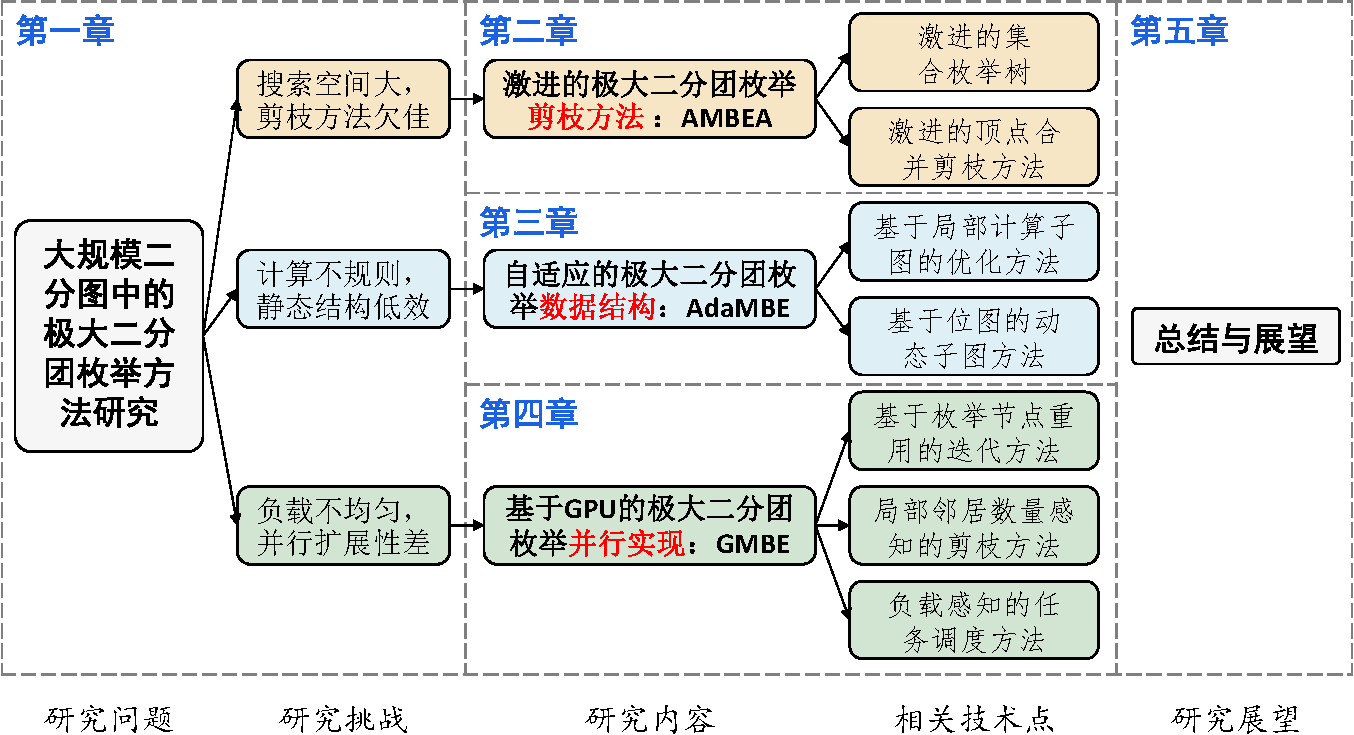
\includegraphics[width=0.82\linewidth]{outline_new}
  \vspace{-0.05 in}
  \caption{本文的组织结构图}
  \label{fig:outline}
\end{figure}

% 第一章作为绪论,介绍了研究背景、研究课题、国内外研究现状和研究挑战,并概述了本文的主要研究内容。考虑到极大二分团枚举在数据挖掘领域和图论领域中的重要应用,我们将本文的研究课题确定为在大规模二分图中的极大二分团枚举方法研究,并

图~\ref{fig:outline}展示了本文的研究内容和结构,共五个章节。
%
第一章作为绪论,首先介绍了研究背景、研究课题以及国内外的研究现状。本文主要研究大规模二分图场景下的极大二分团枚举问题。针对剪枝方法、数据结构和并行实现等三个方面的挑战,本文提出三个高效的算法,分别对应于论文的第二、第三和第四章。
%
第二章提出了AMBEA算法,主要包括激进的集合枚举树和激进的顶点合并剪枝方法两个核心技术点。通过深度优化剪枝方法,AMBEA算法在搜索空间和性能方面相较于现有最优算法有明显提升。
%
第三章提出了AdaMBE算法,主要包括基于局部计算子图的优化方法和基于位图的动态子图方法两个核心技术点。AdaMBE算法根据极大二分团枚举任务中计算子图动态变化的特点,采用自适应的数据结构,在性能上比现有算法有较大提升。
%
第四章提出了GMBE算法,主要包括基于枚举节点重用的迭代方法、局部邻居数量感知的剪枝方法以及负载感知的任务调度方法三个核心技术点。相比于现有算法只能在CPU上实现,GMBE在GPU上实现了较大幅度的性能提升。
%
第五章对全文进行总结,并展望未来的研究方向。












% 第一章介绍了大规模二分图中的极大二分团枚举问题在数据挖掘领域和图论领域中重要作用,以及国内外的相关研究工作现状。

% 第二章详细地介绍了二分图中的极大二分团枚举问题。本章首先给出问题的正式定义与相关符号定义,然后介绍了主流的基于集合枚举树的极大二分团枚举方法,最后指出现有方法现有方法在大规模二分图中进行极大二分团枚举所呈现的低效性问题,具体包含搜索空间优化、数据结构选择以及并行扩展三个方面的挑战。针对这些挑战,本文在第三至第五章分别提出三种不同的解决方案。

% 第二章介绍了激进的极大二分团枚举剪枝方法,以优化搜索空间提升枚举性能。针对现有的极大二分团枚举方法在大规模二分图中仍会产生大量非极大二分团的问题,本章提出了一种激进的集合枚举树和一种激进的顶点合并剪枝方法,并结合上述两种方法形成AMBEA算法。%实验证明,AMBEA算法在大规模二分图中的枚举性能优于现有方法,得益于其高效的剪枝性能。

% 第三章介绍了自适应的极大二分团枚举数据结构,采用混合数据结构以提升枚举性能。针对现有极大二分团枚举方法采用单一数据结构所带来的低效性问题,本章针对位图和邻接表两种数据结构分别提出了不同的计算模式,并结合这两种计算模式形成AdaMBE算法。%实验证明,基于混合数据结构的AdaMBE枚举算法比现有方法更具计算优势。

% 第四章介绍了基于GPU的极大二分团枚举并行实现,利用GPU的大量计算核心极大地缩短了枚举时间。针对现有极大二分团枚举算法只能在基于CPU的计算系统中运行且受限于计算核心数量的计算性能问题,本章提出了基于GPU的极大二分团枚举算法。针对在GPU上进行极大二分团枚举所面临的内存不足、线程分歧以及负载不均问题,本章提出了基于枚举节点重用的迭代方法、局部邻居数量感知的剪枝方法和负载感知的任务调度方法,最终形成GMBE算法。%实验证明,基于GPU的GMBE算法在性能上显著优于现有基于CPU的方法,具有更短的执行时间。

% 第五章对全文进行总结,并展望未来的研究方向。




\chapter{二分图中的极大二分团枚举问题}
\label{ch:intro}

二分图是图论中一种基本结构,被广泛应用于社交网络分析、推荐系统、生物信息学等领域。在二分图中,极大二分团是特殊的子图,用于描述不同群体之间的连接关系,具有重要的研究价值和应用潜力。极大二分团枚举问题在数据挖掘和图论领域中扮演着重要角色,帮助我们理解图的结构和特征,并挖掘有用的信息。例如,在电子商务中,极大二分团可以描述同时购买某批商品的用户群体,通过枚举极大二分团,可以提高对刷单行为的检测率。然而,随着二分图规模的增大,极大二分团的数量也不断增加,如何高效地进行枚举成为一个严峻挑战。本章首先概述二分图中极大二分团枚举问题的定义,随后介绍基于集合枚举树进行极大二分团枚举的基本方法,最后讨论现有方法存在的问题和挑战。

% 二分图是图论中的一种基本结构,广泛应用于许多领域,如社交网络分析、推荐系统、生物信息学等。在二分图中,极大二分团是一种特殊的子图,用来最大程度地描述两个不同群体间的连接关系,具有重要的研究价值和应用潜力。二分图中的极大二分团枚举问题在数据挖掘领域和图论领域中扮演着重要的角色,因为他可以帮助我们更好的理解图的结构和特征,进而从中挖掘有用的信息。例如,在电子商务场景中,极大二分团描述同一批用户同时购买了同一批商品。通过对极大二分团的枚举,便于找到可以交易,提升对刷单行为的检出率。随着大数据时代的到来,二分图的规模不断扩大,极大二分团的数量不断增多,在短时间内完成极大二分团枚举的计算成为了一个严峻的挑战。本章给出了二分图中的极大二分团枚举问题的概述,包括问题定义以及现有方法存在的问题与挑战。

\section{问题定义}

在问题定义之前,我们首先介绍图论领域的一些基础概念,并提供了随后频繁使用的符号及其含义,如表~\ref{tab:definition}所示。

\begin{longtable}[htbp]{|c|p{12cm}|}
    \caption{本文使用的符号及含义}
    \label{tab:definition} \\
    
    \hline
    符号 & 含义 \\ \hline
    \endfirsthead
    
    \hline
    符号 & 含义 \\ \hline
    \endhead
    
    \hline
    \multicolumn{2}{r}{续下页} \\
    \endfoot
    
    \hline
    \endlastfoot
    
    $G(U,V,E)$ & 一个无向二分图 $G$,其中 $U$ 和 $V$ 是两个不相交的顶点集合,$E$ 是二分图的边集合且 $E \subseteq U \times V$。 \\ \hline
    $u,v$ & 表示二分图 $G$ 中的顶点。其中顶点 $u$ 属于集合 $U$,顶点 $v$ 属于集合 $V$。 \\ \hline
    $N(v)$ & 表示顶点 $v$ 的邻居顶点集合,即 $N(v) = \{u \,|\, (u,v) \in E\}$。 \\ \hline
    $N_2(v)$ & 表示顶点 $v$ 的二跳邻居顶点集合,即 $N_2(v) = \bigcup_{u \in N(v)} N(u) - \{v\}$。 \\ \hline
    $\Delta(v)$ & 表示顶点 $v$ 的度数,即 $\Delta(v) = |N(v)|$。 \\ \hline
    $\Gamma(X)$ & 表示顶点集 $X$ 内顶点的共同邻居,即 $\Gamma(X) = \bigcap_{v \in X} N(v)$。 \\ \hline
    $\Upsilon(X)$ & 表示顶点集 $X$ 内顶点的合并邻居,即 $\Upsilon(X) = \bigcup_{v \in X} N(v)$。 \\ \hline
    $\Delta(X)$ & 表示顶点集 $X$ 内顶点的最大度数,即 $\Delta(X) = \max_{u \in X} |N(u)|$。 \\ \hline
    $\Delta_2(X)$ & 表示顶点集 $X$ 内顶点的最大二跳度数,即 $\Delta_2(X) = \max_{u \in X} |N_2(u)|$。 \\ \hline
    $X_v^+, X_v^-$ & 表示顶点集 $X$ 根据顶点 $v$ 划分成的两个子集。给定一个顶点顺序,$X_v^+$ 包含所有顶点比 $v$ 更大的顶点(顺序在 $v$ 之后的顶点),即顶点$v$的尾部顶点;$X_v^-$ 包含包括 $v$ 顶点在内的所有顶点比 $v$ 更小的顶点(顺序在 $v$ 之前的顶点),即顶点$v$的头部顶点。 \\ \hline
    $L,R,C$ & $L$, $R$ 和 $C$ 指三个两两不相交的顶点集,其中 $L$ 是集合 $U$ 的子集,$R$ 和 $C$ 是集合$V$ 的子集。$L,R$ 和 $C$ 共同构成一个枚举树节点,其中 $(L,R)$ 表示枚举树节点对应的二分团,$C$ 表示用于生成新枚举树节点的候选顶点。对于二分团 $(L,R)$,$L$ 和 $R$ 分别表示二分团的左部顶点集和右部顶点集。 \\ \hline
    $N_L(v)$ & 表示顶点 $v$ 的局部邻居。对于对应二分团 $(L,R)$ 的枚举树节点,$N_L(v) = L \cap N(v)$。 \\ \hline
    $\vec{v}$ & 对于一个枚举树节点,$\vec{v}$ 表示用于生成该枚举树节点的候选顶点,即枚举树中从父节点到子节点的边上的遍历候选顶点。 \\ \hline
    $\alpha, \delta, \beta$ & 对于一棵极大二分团枚举树,$\alpha$ 表示枚举树中产生的极大二分团的数量,$\delta$ 表示枚举树中产生的其他二分团的数量,$\beta$ 表示枚举树中二分团的总数量。可知 $\beta = \alpha + \delta$。 \\ \hline
\end{longtable}

  二分图中的极大二分团枚举问题是在一个无向无权二分图$G(U,V,E)$中的特定的图挖掘问题。随后,我们正式定义二分团、极大二分团以及极大二分团枚举问题。

\begin{definition}
  \textbf{(二分团)} 二分团(biclique)是二分图$G(U,V,E)$中的稠密二分子图$(L,R,E')$。其中$L\subseteq U$, $R\subseteq V$, $E' = L \times R \subseteq E$。为了方便,下文中我们直接用顶点集对$(L,R)$表示二分团。
\end{definition}

\begin{definition}
  \textbf{(极大二分团)} 极大二分团(maximal biclique)是二分图$G$中的一个二分团,且该二分团不能再添加其他顶点使其成为更大的二分团。
  \label{def:mb}
\end{definition}

\begin{definition}
  \textbf{(极大二分团枚举问题)} 本文所研究的极大二分团枚举问题(maximal biclique enumeration, MBE)的目标是无重复、无遗漏地枚举二分图中的全部极大二分团。
\end{definition}

\begin{figure} [ht]
  \vspace{0.2 in}
  \centering
  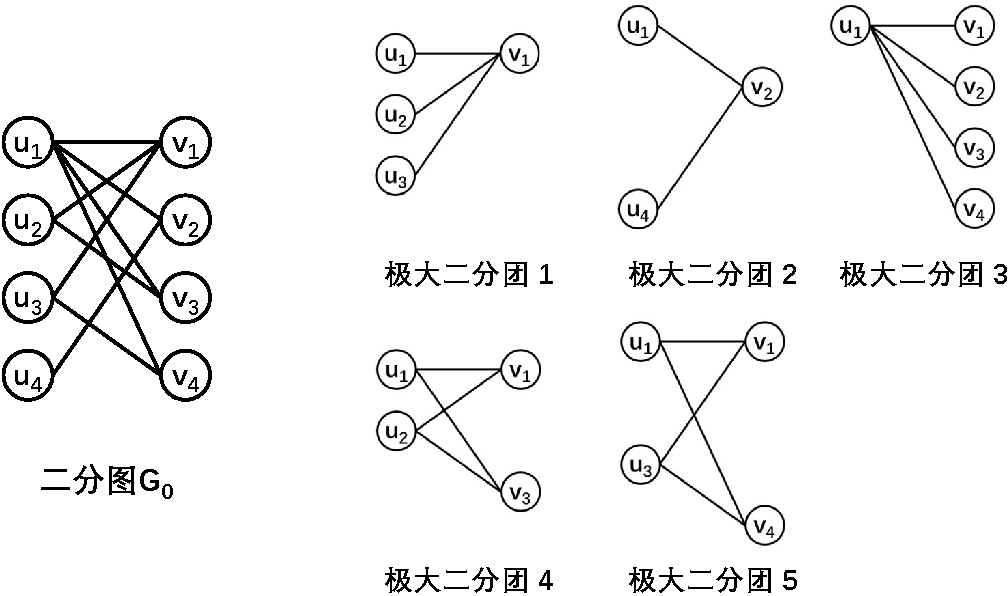
\includegraphics[width=0.8\linewidth]{eg_definition}
  \vspace{0.1 in}
  \caption{二分图中的极大二分团枚举问题示例}
  \label{fig:eg_definition}
\end{figure}

\begin{example}
  图~\ref{fig:eg_definition}给出了一个二分图中的极大二分团枚举问题的示例。其中左图是一个具有8个顶点,9条边的二分图$G_0$,右图展示了二分图中的全部极大二分团,共5个。极大二分团枚举问题即无重复、无遗漏地枚举二分图$G_0$中的全部5个极大二分团。
  
\end{example}

\section{基于集合枚举树的极大二分团枚举方法}
\label{sec:se}


集合枚举树是解决集合问题的强大工具,在主流的极大二分团枚举算法中扮演着重要角色。本节将详细介绍集合枚举树,并介绍基于该树的极大二分团枚举算法,并分析其算法复杂度。


\begin{figure} [ht]
  \vspace{0.1 in}
  \centering
  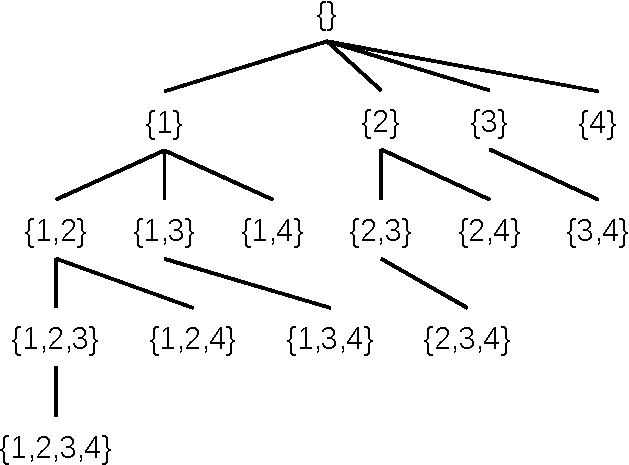
\includegraphics[width=0.55\linewidth]{se_naive}
  \vspace{0.15 in}
  \caption{对于集合$P\{1,2,3,4\}$的集合枚举树}
  \label{fig:se_naive}
\end{figure}




\subsection{集合枚举树介绍}
\label{subsec:se}


\textbf{集合枚举树}(set enumeration tree, SE tree)是一种用于有序地枚举特定集合全部子集的数据结构,即枚举该集合的幂集~\cite{SEtree92}。它为解决搜索空间为特定集合幂集的子集的问题提供了一种完整且无冗余的搜索技术。具体而言,集合枚举树如图~\ref{fig:se_naive} 所示,根节点表示空集,每个节点对应一个子集,其子节点代表在该子集基础上添加一个新元素所得到的子集。对于二分图中的极大二分团枚举问题而言,每个二分团的集合$R$即为二分图中集合$V$的一个独特子集。因此,通过引入集合枚举树可以无重复、无遗漏地枚举全部可能的极大二分团,进而有效地求解极大二分团枚举问题。

对于应用于极大二分团枚举问题的集合枚举树,我们从以下三个角度对其进行了规范化描述:

\begin{itemize}
  \item 节点结构:每个树节点为一个三元组$(L,R,C)$。在一个二分图$G(U,V,E)$,集合$L$是集合$U$的子集,集合$R$和集合$C$是集合$V$的两个不相交子集。集合$L$和$R$构成一个二分团,其中集合$L$包含左部顶点,集合$R$包含右部顶点。集合$C$包含用于扩展集合$R$的候选顶点。
  \item 节点生成:枚举树从根节点$(U,\emptyset,V)$ 开始遍历。对于当前节点$(L,R,C)$,枚举树按顺序访问集合$C$中的每个候选顶点$v'$以生成一个新的节点$(L',R',C')$。集合$L'$包含集合$L$和集合$N(v')$中的共同顶点。集合$R'$包含集合$R$中的顶点、顶点$v'$以及集合$C$中与集合$L'$内顶点均相连且未被访问的顶点。集合$C'$包含集合$C$中与集合$L'$内顶点部分相连的且未被访问的顶点。
  \item 节点检查:当且仅当集合$L'$的共同邻居等于集合$R'$, 即$\Gamma(L')=R'$时,节点$(L',R',C')$通过节点检查,输出一个极大二分团。
\end{itemize}

此外,一些研究~\cite{iMBEA14,ooMBE22}在每个枚举节点中额外引入集合$Q$作为辅助节点检查的工具,构成四元组$(L,R,C,Q)$。其中集合$Q$于存储已访问的候选顶点,以帮助检查节点是否对应非极大二分团。具体而言,当集合$Q$中存在任意一个顶点$v_q$,并且它的邻居包含了集合$L$中的所有顶点时,根据定义~\ref{def:mb}我们可以推断当前节点对应的二分团$(L,R)$可以添加顶点$v_q$构成新的二分团,即$(L, R\cup\{v_q\})$,从而我们可以判定当前节点对应一个非极大二分团。然而,使用集合$Q$需要额外的存储和计算开销。幸运的是,我们观察到可以通过访问$L$中的任意顶点$u_l$的邻居$N(u_l)$来高效地替代集合$Q$的作用。具体而言,当集合$N(u_l)$中存在一个不在$R$集合中的顶点$v^*$,并且它的邻居包含了集合$L$中的所有顶点时,我们可以推断当前节点对应的二分团$(L,R)$可以添加顶点$v^*$构成新的二分团,从而判定当前节点对应一个非极大二分团。因此,在枚举树的介绍和相关算法中,我们不再引入集合$Q$。

\subsection{基于集合枚举树的极大二分团枚举算法}
\label{subsec:algorithm}
根据前一节对应用于极大二分团枚举问题的集合枚举树的描述,我们给出了基于集合枚举树的极大二分团枚举的算法。

\begin{algorithm}[H]
    \begin{algorithmic}[1]
        \normalsize
        \REQUIRE 二分图 $G(U,V,E)$
        \ENSURE 所有极大二分团
        
        \renewcommand{\algorithmicwhile}{\textbf{procedure}}
        \renewcommand{\algorithmicdo}{\textbf{:}}


        \STATE \textsf{biclique\_search\_basic}$(U,\emptyset,V)$;
        \WHILE{\textsf{biclique\_search\_basic}$(L,R,C)$}
        \renewcommand{\algorithmicdo}{\textbf{do}}
          \FOR{$v' \in C$}
            \STATE $L' \leftarrow L \cap N(v')$; $R'\leftarrow R$; $C' \leftarrow \emptyset$;
            \FOR{$v_c \in C$}
              \IF{$L' \cap N(v_c) = L'$}
                \STATE $R' \leftarrow R' \cup \{v_c\}$;
              \ELSIF{$L' \cap N(v_c) \neq \emptyset$}
                \STATE $C' \leftarrow C' \cup \{v_c\}$;
              \ENDIF
            \ENDFOR
            \IF{$\Gamma(L') = R'$}
              \STATE 输出极大二分团$(L', R')$;
              \STATE \textsf{biclique\_search\_basic}$(L',R',C')$;
            \ENDIF
            \STATE $C \leftarrow C \setminus \{v'\}; $
          \ENDFOR

        \ENDWHILE

    \end{algorithmic}
    \caption{基于集合枚举树的MBE算法}
    \label{alg:se_mbe}
\end{algorithm}

算法~\ref{alg:se_mbe}总结了基于集合枚举树的极大二分团枚举算法的基本枚举过程。具体而言,该算法从根节点$(U,\emptyset,V)$开始,递归地调用\textsf{biclique\_search\_basic}过程 (第1行)。过程\textsf{biclique\_search\_basic}接收一个枚举树节点作为输入,即该节点对应的集合$L$,$R$和$C$ (第2行)。在处理当前枚举节点时,该过程会逐个遍历$C$中的顶点$v'$ (第3行),然后根据集合枚举树的节点生成规则生成新节点$(L',R',C')$ (第4-11行)。随后,过程按照节点检查规则对新生成的节点$(L',R',C')$进行检查 (第12行)。如果该节点对应一个极大二分团,则输出该二分团 (第13行),并递归地调用过程\textsf{biclique\_search\_basic}以节点$(L',R',C')$为根节点继续探索子枚举树 (第14行);否则,我们知道该节点对应非极大二分团,跳过该节点。为保证$C$中的顶点都未被访问,过程会及时从$C$中移除已访问的顶点$v'$ (第16行)。我们用下面的例子对该算法进行说明。


\begin{figure} [ht]
  \vspace{0.1 in}
  \centering
  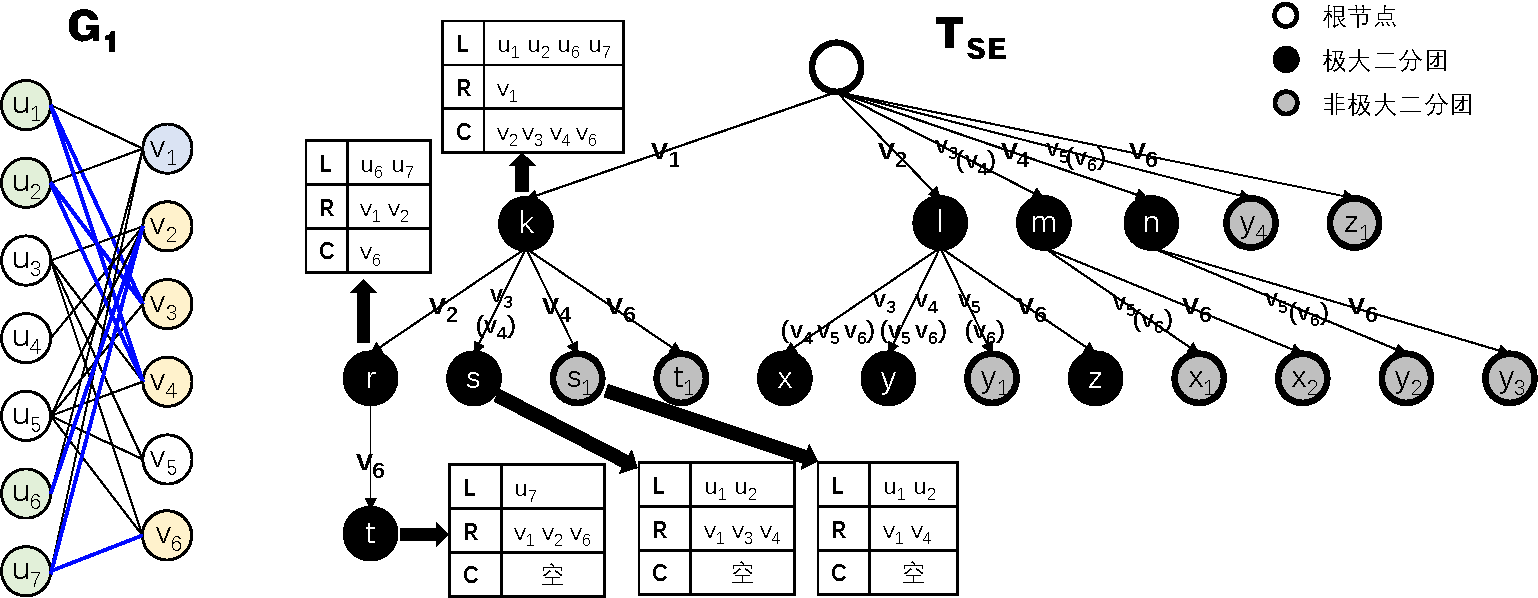
\includegraphics[width=0.95\linewidth]{se_mbea}
  \vspace{0.1 in}
  \caption{算法~\ref{alg:se_mbe}在二分图$G_1$上的集合枚举树}
  \label{fig:se_mbea}
\end{figure}

\begin{example}
  \label{example:se}
  图~\ref{fig:se_mbea}展示了算法~\ref{alg:se_mbe}在二分图$G_1$上的集合枚举树$T_{SE}$。
  \footnote{为了方便比较,整个文中具有相同字母标识的节点在枚举树中共享相同的集合$L$,只有没有下标的节点会输出极大二分团。例如,节点$s$和节点$s_1$具有相同的集合$L$,但只有节点$s$会输出一个极大二分团。我们使用集合的下标来表示该集合隶属于哪个节点。例如$L_s$表示节点$s$的集合$L$。 
}
我们从根节点开始,通过深度优先搜索逐个遍历候选顶点,递归地搜索子空间。首先,我们通过遍历顶点$v_1$生成节点$k$。按照算法~\ref{alg:se_mbe}中第4-11行的计算方法,我们可以计算得到$L_k=N(v_1)=\{u_1, u_2, u_6, u_7\}$,$R_k=\{v_1\}$,$C_k=\{v_2,v_3,v_4,v_6\}$。根据节点检查规则,因为$\Gamma(L_{k}) = \{v_1\} = R_{k}$,所以节点$k$输出一个极大二分团并继续探索以节点$k$为根节点的子枚举树。为便于观察,我们在图$G_1$中标记了节点$k$中的顶点,即$L_k$,$R_k$和$C_k$中的全部顶点,并标出了集合$L_k$与集合$C_k$之间的边。

接下来,节点$k$遍历顶点$v_2$生成节点$r$。同理,我们可以计算得到$L_{r} = N(v_2) \cap L_{k} 
= \{u_3, u_4, u_5, u_6, u_7\} \cap \{u_1, u_2, u_6, u_7\} = \{u_6, u_7\}$, $R_{r} = R_{k} \cup (C_{k} \cap \Gamma(L_{r})) = \{v_1\} \cup (\{v_2, v_3, v_4, v_5\} \cap \{v_1, v_2\}) = \{v_1, v_2\}$。集合$C_{r}$中仅包含顶点 $v_6$,因为顶点$v_3$, $v_4$和 $v_5$不与集合$L$中的任何顶点相连。

继续这个过程,我们可以计算得到节点$s$以及节点$s_1$。节点$s$对应二分团$(\{u_1, u_2\},$ $\{v_1, v_3, v_4\})$,节点$s_1$对应二分团 $(\{u_1, u_2\}, \{v_1, v_4\})$。根据节点检查规则,因为$\Gamma(L_{s_1}) = \{v_1, v_3, v_4\} \neq R_{s_1} = \{v_1, v_4\}$,所以节点$s_1$对应一个非极大二分团。具体地,与节点$s$相比,节点$s_1$不能用$v_3$来扩展该节点中的集合$R_{s_1}$。这是因为在生成节点$s_1$时,根据深度优先搜索的规则,顶点$v_3$已被访问并用于生成节点$s$。因此,在节点检查之后,我们删除了节点$s_1$。同理,其他节点可以类似地生成。

\end{example}

在算法~\ref{alg:se_mbe}的基础上,现有的基于枚举树的极大二分团枚举算法的优化方法主要包括变节点候选顶点的遍历顺序~\cite{minel06,iMBEA14,PMBE20,ooMBE22}、设计剪枝方法以提前裁剪产生非极大二分团的节点~\cite{iMBEA14,PMBE20,ooMBE22},以及并行优化~\cite{mapreduceMBE16,parMBE19}。在~\ref{sec:opt}节中,我们将对上述优化方法进行详细说明,并介绍它们在实际应用中的效果。

\subsection{算法复杂度分析}
\label{subsec:baseline_analysis}

本节从时间复杂度和空间复杂度两个方面对算法~\ref{alg:se_mbe}进行分析。

\textbf{时间复杂度:} 我们首先分析枚举树中每个节点的计算时间,随后分析枚举树中的枚举节点数量,最终得到算法~\ref{alg:se_mbe}的时间复杂度。平均而言,对于每个节点$(L',R',C')$的计算包括节点生成(第4-11行)和节点检查(第12行)两个部分。由于集合$C$中最多包含$|V|$个顶点,且每个顶点的集合交集运算需要$O(\Delta(V))$的时间,因此节点生成过程的时间复杂度为$O(|V|\Delta(V))$。而节点检查过程中,我们可以通过只访问二分图中的每条边一次来获取$\Gamma(L')$的值,因此节点检查的时间复杂度为$O(|E|)$(或$O(|V|\Delta_{avg}(V))$)。综上,每个节点的计算时间为$O(|V|\Delta(V))$。为了量化算法的计算时间,我们用$\beta$来表示枚举树中节点的数量。最终,算法的时间复杂度为$O(|V|\Delta(V)\beta)$。

\textbf{空间复杂度:} 由于算法~\ref{alg:se_mbe}按照深度优先的方式进行搜索,我们可以对枚举树中每个节点占用的空间进行分析,并结合枚举树的高度以及输入二分图所占用的空间,得到算法的空间复杂度。对于每个节点$(L',R',C')$,集合$L'$最多包含$\Delta(V)$个顶点,集合$R'$和$C'$最多包含$|V|$个顶点。在二分图中,集合$V$内顶点的数量通常远高于任何单个顶点的度数,因此每个节点的空间开销为$O(\Delta(V)+|V|)=O(|V|)$。在递归过程中,节点的集合$L$内的顶点数量不断减少,因此我们可以确定枚举树的高度为$O(\Delta(V))$。考虑到二分图$G(U,V,E)$需要占用$O(|U|+|V|+|E|)=O(|E|)$的空间,最终算法的空间复杂度为$O(|E|+|V|\Delta(V))$。

\section{存在的问题与挑战}

尽管在极大二分团枚举领域已经有很多出色的工作,但是在处理大规模二分图时,已有方法的计算性能仍然有很大的提升空间。本节将指出现有基于集合枚举树的枚举方法所面临的三个共性问题,并介绍解决这些问题所面临的具体挑战。

\subsection{搜索空间大,剪枝方法欠佳}

极大二分团枚举问题具有搜索空间大的特点。常见的图算法,如深度优先搜索~\cite{wiki-dfs}、广度优先搜索~\cite{wiki-bfs}、最小生成树~\cite{wiki-mst}、最短路径等算法~\cite{wiki-sssp},其搜索空间随着图的规模线性增长。常见的图模式挖掘算法的目标子图往往只包含少量顶点~\cite{peregrine20,pangolin20,g2miner22,decomine22,khuzdul23,gamma23,Graphset23},例如三角计数问题中目标子图仅包含3个顶点~\cite{triangle18}。相比之下,极大二分团枚举问题的搜索空间更大,因为它随着二分图中顶点数量的指数级增长,并且目标子图(即极大二分团)中的顶点数量相对较多。为了应对搜索空间巨大的挑战,研究人员提出了各种优化技术,旨在减少搜索空间中产生非极大二分团的无效枚举节点,进而减少枚举时间。然而,由于搜索空间的规模庞大,现有的优化方法往往难以完全覆盖所有无效节点。具体而言,通过~\ref{subsec:ambea_exp_overall}节的实验,我们观察到现有的最新算法ooMBEA在Github数据集上需要检查并消除比极大二分团数量多26倍的产生非极大二分团的无效枚举节点。这些无效枚举节点带来大量的节点检查开销,严重降低了计算性能。因此,如何设计高效的剪枝方法来裁剪巨大搜索空间仍然是一个关键的挑战。


\subsection{计算不规则,单一结构低效}

极大二分团枚举问题具有计算不规则的特点。与其他图计算问题类似,在真实世界中,二分图的顶点邻居数量存在较大差异,导致每次计算涉及的顶点数量不同,即计算不规则~\cite{Irregularity12}。为了高效地解决这类问题,研究者们提出了多种存储结构来表示图的邻接关系。常用的存储结构包括位图~\cite{lcm04,lcmmbc07,FCA15,FCA21,FCA22}、邻接表~\cite{iMBEA14,PMBE20,ooMBE22}和哈希表~\cite{parMBE19}。不同的存储结构适用于不同场景。
例如,位图结构采用位运算,具有高效的计算能力,但在稀疏图场景下会占用更多的存储资源,因此适用于稠密小图;邻接表精确地存储每个顶点的邻居信息,在处理稀疏大图时占用较少的内存,但计算过程需要执行大量的比较运算,其运行时间与顶点个数成正比,会导致计算相对低效,因此适用于稀疏大图;哈希表具有灵活性和便于快速查找的特点,可以快速判断任意两个顶点之间的连接关系,但相比邻接表,它需要更多的存储空间并且访问方式更为随机。然而,目前的研究往往采用固定的数据结构来存储顶点的邻居信息,未能充分发挥不同数据结构的优势。因此,在枚举过程中如何动态选择合适的存储结构,发挥计算潜力,是一个关键挑战。



\subsection{负载不均匀,并行扩展性差}

极大二分团枚举问题具有负载不均匀的特点,限制了问题的并行扩展能力。为了进一步提高问题求解的效率,研究人员尝试设计并行算法来处理极大二分团枚举问题~\cite{mapreduceMBE16, MBEHe18, parMBE19}。这些算法将整个集合枚举树分解成多个子枚举树,然后利用分布式系统或多核CPU的大量计算资源来并行处理这些子树。然而,由于不同子枚举树的极大二分团的大小不同,导致计算负载之间存在较大差异。因此,即使有大量计算资源可用,计算任务的运行时间仍然受限于最耗时的负载。GPU作为一种专门用于并行计算的硬件设备,由于其内部拥有大量的计算单元,非常适合处理并行任务。然而,由于GPU和CPU在体系结构、内存层次结构以及编程模型等方面存在较大差异,现有的极大二分团枚举算法无法直接迁移到GPU系统中。尽管GPU被广泛用于加速相关的图算法,如极大团枚举~\cite{MCEGPUBitset13,MCEGPUdpp17,MCE-GPU21} 和图模式挖掘~\cite{g2miner22,SubgraphGpu22,Kclique22,stmatch22},但在GPU上进行极大二分团枚举问题仍然具有挑战性。具体来说,GPU上的极大二分团枚举问题面临着与极大二分团枚举问题类似的性能问题,许绍显等人指出GPU加速极大团枚举问题的研究极为有限~\cite{MCEreview22}。即使最新的基于GPU的极大团枚举算法GBK~\cite{MCE-GPU21} 获得较低的性能,也仅与CPU上的单线程串行算法相当。GPU上的子图枚举问题中被枚举子图通常仅包含少量顶点,而极大二分团通常包含大量顶点,因此带来更加严重的负载不均问题,导致最新的基于GPU的GPM框架G$^2$Miner~\cite{g2miner22}与GraphSet~\cite{Graphset23}中的优化无法直接解决GPU上进行极大二分团枚举面临的负载不均匀问题。因此,如何实现负载均衡并突破现有算法在并行能力方面的限制,设计基于GPU的并行极大二分团枚举方法是一个重要挑战。



\section{本章小结}

本章首先介绍了二分图中的极大二分团枚举问题的定义。随后结合伪代码以及实例介绍了基于集合枚举树的极大二分团枚举基本方法,并对算法复杂度进行分析。最后针对极大二分团枚举问题的搜索空间大、计算不规则以及负载不均匀三个特点,指出现有方法存在的问题与挑战。
\chapter{激进的极大二分团枚举剪枝方法}
\label{ch:aggressive_mbe}

\section{本章介绍}
\section{背景知识}
\label{sec:opt}

用于极大二分团枚举的集合枚举树

现有优化方法分析


\begin{table} 

  \caption{基于集合枚举树的极大二分团枚举的现有优化方法}
  \label{tbl:sota}
  %\normalsize
  \centering
  
  \begin{tabular}{|c|p{10cm}|}\toprule
    \hline
    \textbf{优化方法} & \multicolumn{1}{c|}{\textbf{相关工作}} \\ \hline
优化顶点的遍历顺序~\cite{iMBEA14,PMBE20,ooMBE22} & 在基于集合枚举树的枚举方法中,可以自由选择顶点的遍历顺序。Zhang等人按顶点的邻居数量进行升序排序~\cite{iMBEA14}。Abidi等人利用索引结构CDAG,按逆拓扑顺序排序~\cite{PMBE20}。Chen等人利用单边顺序控制候选顶点的数量上限,按单边顺序排序~\cite{ooMBE22}。\\ \hline
剪枝优化策略~\cite{iMBEA14,PMBE20,ooMBE22} & 利用运行时候选顶点间的内在联系,对即将生成无效二分团的候选顶点进行裁剪。Zhang等人裁剪与正在遍历顶点邻居相同的候选顶点~\cite{iMBEA14}。Abidi等人建立全局索引结构CDAG,利用枢纽顶点与其他顶点的包含关系进行剪枝~\cite{PMBE20}。Chen等人提出批量枢纽技术,对无效分支进行批量裁剪~\cite{ooMBE22}。\\ \hline
并行优化策略~\cite{mapreduceMBE16,parMBE18} & 基于分布式集群或多核CPU实现的极大二分团枚举并行优化。Mukherjee等人利用MapReduce实现了分布式枚举算法,但多节点通信开销可能降低性能~\cite{mapreduceMBE16}。Das等人利用多核CPU实现了多线程枚举算法,但性能受限于CPU计算核数量~\cite{parMBE18}。 \\ \hline

  \end{tabular}
    
\end{table}


\section{研究动机}

\section{AMBEA算法设计与实现}

\subsection{激进的集合枚举树}

\subsection{激进的顶点融合剪枝方法}

\subsection{AMBEA算法}

\section{实验评估}

\subsection{实验设置}

\subsection{整体评估}
\label{subsec:ambea_exp_overall}

\subsection{细分评估}

\subsection{敏感性测试}

\section{本章小结}
\chapter{自适应的极大二分团枚举数据结构}
\label{ch:adapt_mbe}

针对极大二分团枚举问题中单一数据结构低效的问题,本章整理了相关工作中所涉及的不同的图存储数据结构,详细描述不同数据结构的优劣以及适用场景,并指出单一数据结构所导致的局限性作为本章的研究动机。本章结合不同数据结构的优势以及极大二分团枚举问题的特点,提出了以下优化方法:首先,






\section{背景知识}
二分图数据结构

\section{研究动机}

\section{AdaptMBE算法设计与实现}

\subsection{基于位图的子图计算模式}

\subsection{基于邻接表的横向计算模式}

\subsection{AdaptMBE算法}

\section{实验评估}

\subsection{实验设置}

\subsection{整体评估}

\subsection{细分评估}

\subsection{敏感性测试}

\section{本章小结}
\chapter{基于GPU的极大二分团枚举算法}
\label{ch:gmbe}

针对现有极大二分团枚举算法在并行扩展性方面受限于CPU计算核心数量的问题,本章引入了具有大量计算核心的GPU作为计算资源,以加速极大二分团枚举过程。本章介绍了现代GPU的硬件架构和软件编程模型。同时,本章%整理了GPU加速图计算的相关工作,并
指出在GPU上实现极大二分团枚举所面临的挑战,作为研究的动机。具体而言,简单地将现有算法映射到大量的GPU计算核心中会遇到内存短缺、线程分歧和负载不均等问题。为了解决这些问题,本章提出了以下优化方法:首先,针对内存短缺问题,本章提出了基于枚举节点重用的迭代方法。该方法可以重用枚举树根节点内存,避免为新枚举节点动态分配内存,从而减少内存开销。其次,针对线程分歧问题,本章提出了局部邻居数量感知的剪枝方法。该方法通过记录枚举过程中顶点局部邻居数量的变化对枚举空间进行剪枝,缓解了线程分歧问题。然后,针对负载不均问题,本章提出了负载感知的任务调度方法。该方法将每棵子枚举树对应的计算任务与一个线程束的计算资源进行绑定,在运行时动态预估子枚举树的大小并对较大的子枚举树进行进一步拆分,实现了细粒度的负载均衡。最后,本章结合上述三种方法,提出了基于GPU的高效极大二分团枚举解决方案GMBE。实验证明,基于单个NVIDIA A100 GPU的GMBE相比现有基于96个CPU的并行算法ParMBE实现了70.6倍的性能提升。

\section{现代GPU架构与编程模型} 
\label{sec:gpu_arch}
GPU,即图形处理单元(Graphics Processing Unit),最初是专门用于处理图形数据的处理器。随着计算需求的增加,现代GPU逐渐演变成了通用并行处理器,能够高效执行大规模数据并行计算任务,如科学计算、深度学习和密码学等。与传统的中央处理器(Central Processing Unit,CPU)相比,现代GPU拥有更多的计算核心,并且能够利用这些核心并行处理大量数据,因此成为加速图计算的有力工具,同时具备加速极大二分团枚举问题的潜力。在本节中,我们将深入探讨现代GPU的硬件架构、与硬件架构对应的主流的软件编程模型CUDA (Compute Unified Device Architecture) 以及针对CUDA的编程指南,作为本章的研究背景。

\begin{figure} [t]
  \center
    % \vspace{0.1in}
		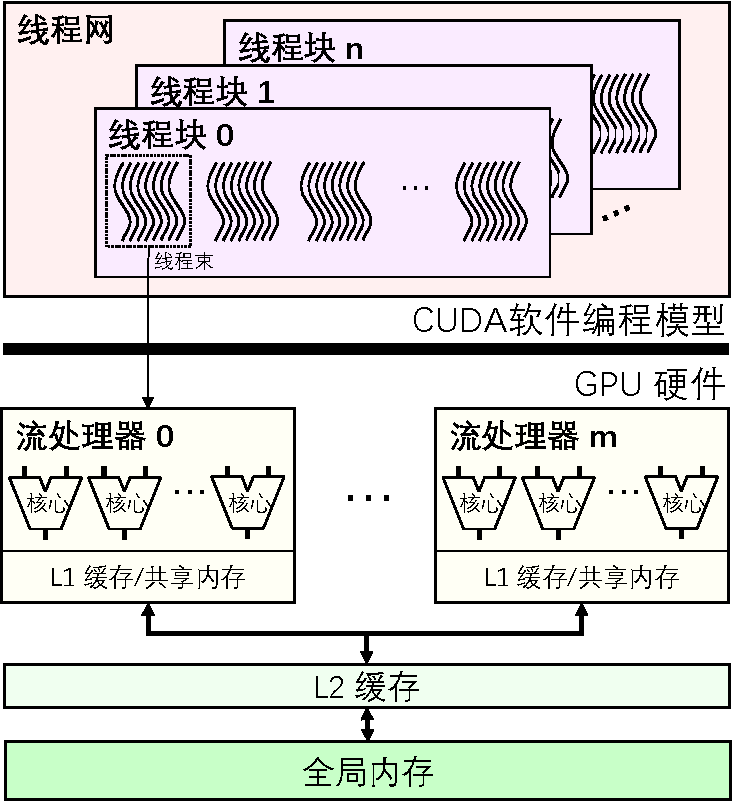
\includegraphics[width=0.55\linewidth]{gpu_arch}
     \vspace{-0.1in}
	\caption{现代GPU硬件架构与软件编程模型}
	\label{fig:gpu}
\end{figure}

图\ref{fig:gpu}展示了现代GPU的硬件架构和软件编程模型。GPU的\textbf{硬件架构}包括大量的计算核心,以及对应的层级存储结构。具体而言,一块现代GPU通常包括全局内存(Global Memory)、共享的L2缓存(Cache)以及大量的流处理器 (Streaming Multiprocessor, SM)。每个流处理器包含单独的L1缓存、可编程的具有多分区(Multi-bank)的共享内存(Shared Memory),以及多个轻量级计算核心(Core)。主流的GPU可以配备上万个轻量级计算核心,提供了巨大的计算能力。然而,与丰富的计算资源相比,GPU上的内存资源相对有限。例如,近年备受青睐的NVIDIA A100~\cite{NVIDIA-A100}最多可以提供6912个核心,但只能提供最多80GB的全局内存。

与GPU的多计算核心的硬件架构相对应,主流的\textbf{CUDA软件编程模型}按照层级结构管理大量线程。具体而言,CUDA编程模型提供了一个并行计算平台和一组API~\cite{CUDA-wiki,CUDAProgrammingGuide},允许用户高效地利用GPU进行通用目的的处理。CUDA采用SIMT (Single Instruction, Multiple Threads)~\cite{SIMT-wiki}执行模型来管理大量线程。它将GPU内核划分为多个线程网(Grid),每个线程网包含多个线程块(Block),每个线程块包括多个线程(Thread),并在执行期间分配给一个流处理器(SM)。流处理器将32个并行线程分组成一个线程束(Warp),并同时执行多个线程束。通过这种方式,成千上万个GPU核心可以高效地并行工作,实现高性能计算。




为了提升GPU的执行性效率,我们针对CUDA编程模型总结了\textbf{编程指南}如下:

\begin{figure} [t]
  \center
    % \vspace{0.05in}
		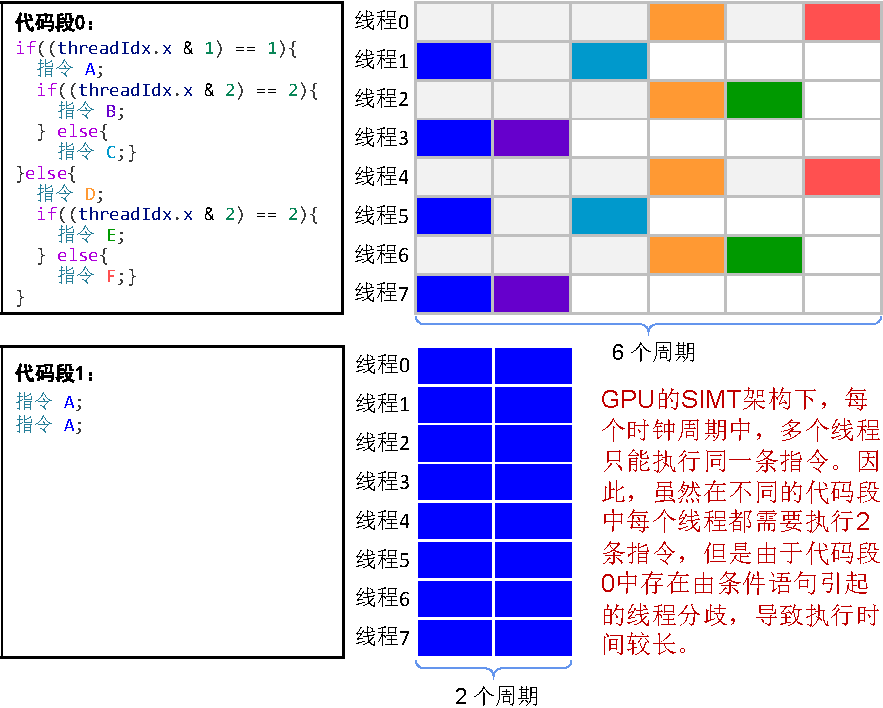
\includegraphics[width=0.8\linewidth]{gmbe/motivation_divergence}
    % \vspace{0.05in}
	\caption{线程分歧示意图}
	\label{fig:gmbe_motivation_divergence}
\end{figure}



\begin{enumerate}
  \item 减少动态内存分配。动态内存分配是指程序在运行过程中动态申请和释放内存。由于 GPU 允许大量的线程同时并发执行,大量线程可能会同时进行动态内存分配,从而引发线程争用、同步开销以及内存碎片化等问题,影响程序性能 ~\cite{DynamicMallocGpu21}。为了避免这种情况的发生,建议采用静态内存分配方式,在程序开始前预估程序的内存使用情况并一次性分配一块足够大的内存,然后在运行时重复使用这块内存,避免频繁的动态内存分配和释放,以降低内存管理的开销并优化内存访问效率。
  
  \item 减少线程分歧。线程分歧是指在 GPU 中同一线程束内的线程执行不同的代码路径。如图~\ref{fig:gmbe_motivation_divergence}所示,由于 GPU 使用 SIMT 的执行模式,即多个线程共享同一组指令,线程分歧会使 GPU 对不同执行路径进行串行化,导致部分线程处于空闲状态,从而严重影响执行性能 ~\cite{CUDAProgrammingGuide}。因此,在CUDA程序应设计简洁的算法和内核函数,尽量保持线程之间的执行路径相似,避免条件语句中大量的分支情况。可以考虑使用线程块内的协作和同步机制来避免线程分歧,尽量使每个线程束内的线程保持一致的执行路径,从而提高并行执行效率。
  

  \item 平衡大量负载。平衡大量负载是指合理地分配计算任务和数据处理任务,确保每个处理单元的负载均衡,避免某些处理单元负载过重而导致性能瓶颈。由于 GPU 拥有大量轻量级计算核心,负载不平衡会导致数千个计算核心等待最慢的计算核心执行,造成严重的资源浪费~\cite{CUDAProgrammingGuide}。为了实现负载平衡,可以考虑将任务划分为较小的子任务,并合理分配给不同的处理单元,通过动态调整任务分配策略来实现计算任务在不同计算资源上的均匀分布,从而提高整体计算效率。此外,可以利用CUDA提供的性能分析工具来帮助识别和解决负载不平衡的问题~\cite{Nsight,CUDANsightSystems,CUDANsightProfile},从而优化程序的性能表现。
  
\end{enumerate}


\section{研究动机}

尽管GPU具有强大的并行能力,在部分图挖掘问题上已经显示出加速效果,但在GPU上实现高效的极大二分团枚举仍然面临严峻的挑战。具体而言,这些挑战主要包括的内存短缺、线程分歧和负载不均等。本节将结合GPU加速图计算的相关工作,对上述挑战进行详细说明。为了方便表述,本章中总是以算法~\ref{alg:se_mbe} 在二分图$G_3$上的集合枚举树为例,如图~\ref{fig:gmbe_tree}所示。

\begin{figure} [H]
	\centering
  \vspace{0.1in}
	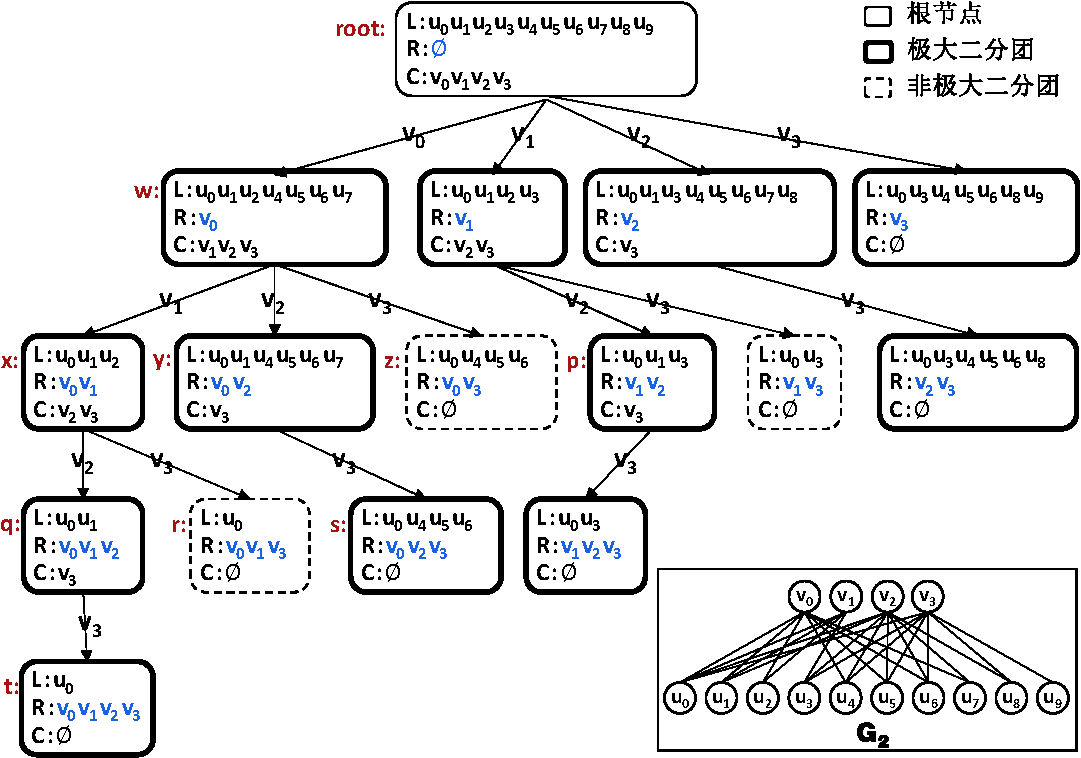
\includegraphics[width=0.9\linewidth]{gmbe/eg_tree}
  \vspace{0.1in}
	\caption{算法~\ref{alg:se_mbe}在二分图$G_3$上的集合枚举树}

	\label{fig:gmbe_tree}
\end{figure}

\subsection{内存短缺}
根据~\ref{subsec:algorithm}节的描述,我们注意到现有的极大二分团枚举算法(如算法~\ref{alg:se_mbe}所示)在枚举过程中会\emph{动态的生成和释放枚举节点$(L,R,C)$}。因此,直接将这类算法迁移到GPU上会导致~\ref{sec:gpu_arch}节中提到的动态内存分配问题。为了实现高性能,现有的基于GPU的图挖掘算法(例如~\cite{MCE-GPU21,Kclique22,g2miner22,Graphset23})通常在执行之前就在GPU上预先分配足够的内存空间来容纳所有的枚举节点。参考这些算法的内存估计方法,我们可以得出在极大二分团枚举算法中,每个枚举节点需要使用$O(|L|+|R|+|C|)$的内存,上限为$O(\Delta(V) + \Delta_2(V))$。同时,在遍历过程中,每棵子树最多需要保存$\Delta(V)$个活跃枚举节点用于回溯。因此,每棵枚举树的遍历过程需要预分配的内存总量为$\Delta(V) \times (\Delta(V) + \Delta_2(V))$ $\times$ \textit{顶点大小}。举例来说,在使用 NVIDIA A100 GPU(40 GB 内存)对真实世界的二分图 BookCrossing~\cite{konect} 进行极大二分团枚举时,每棵子树遍历过程的内存需求为$13,601 \times (13,601 + 53,915) \times$ \textbf{sizeof}(\textbf{int}) B = 3.67\,GB。为了充分利用NVIDIA A100 GPU中的108个流处理器 (SM), 我们需要$108 \times 3.67$ GB = 397 GB的内存,这超过了GPU中的内存空间 (40 GB),因此面临严重的内存短缺问题。

\subsection{线程分歧}
\label{subsec:gmbe_thread_divergence}

由于图挖掘算法本身的不规则性~\cite{Irregularity12},极大二分团枚举算法\emph{涉及大量的分支语句},这导致了~\ref{sec:gpu_arch}节所提到的线程分歧问题。在GPU上进行极大二分团枚举时,线程分歧主要来源于两个方面。首先,在极大二分团枚举过程中,同一线程束内的线程可能会同时访问不同的顶点以生成新节点,并使用不同顶点的邻居来计算不同的集合$L$、$R$和$C$,从而导致不同线程执行不同的控制流以访问不同内存区域。其次,如~\ref{sec:opt}节所述,现有的搜索空间优化方法通常会引入额外的判断语句来对搜索空间进行剪枝,导致不同线程执行路径差异,进一步加剧了线程分歧问题。举例来说,ooMBEA算法~\cite{ooMBE22} 需要访问所有候选顶点的2跳邻居来识别批量枢纽(Batch Pivots),并剪掉不属于批量枢纽的候选顶点,以实现剪枝目的。然而,访问顶点的2跳邻居需要进行深度为2的深度优先搜索,这个过程会涉及到大量对不同顶点邻居边界的条件判断,因而导致更严重的线程分歧问题。因此,在优化枚举空间的同时减少线程分歧是一项具有挑战性的任务,开发适用于GPU的剪枝方法至关重要。

\begin{figure} [H]
  \center
    \vspace{0.1in}
		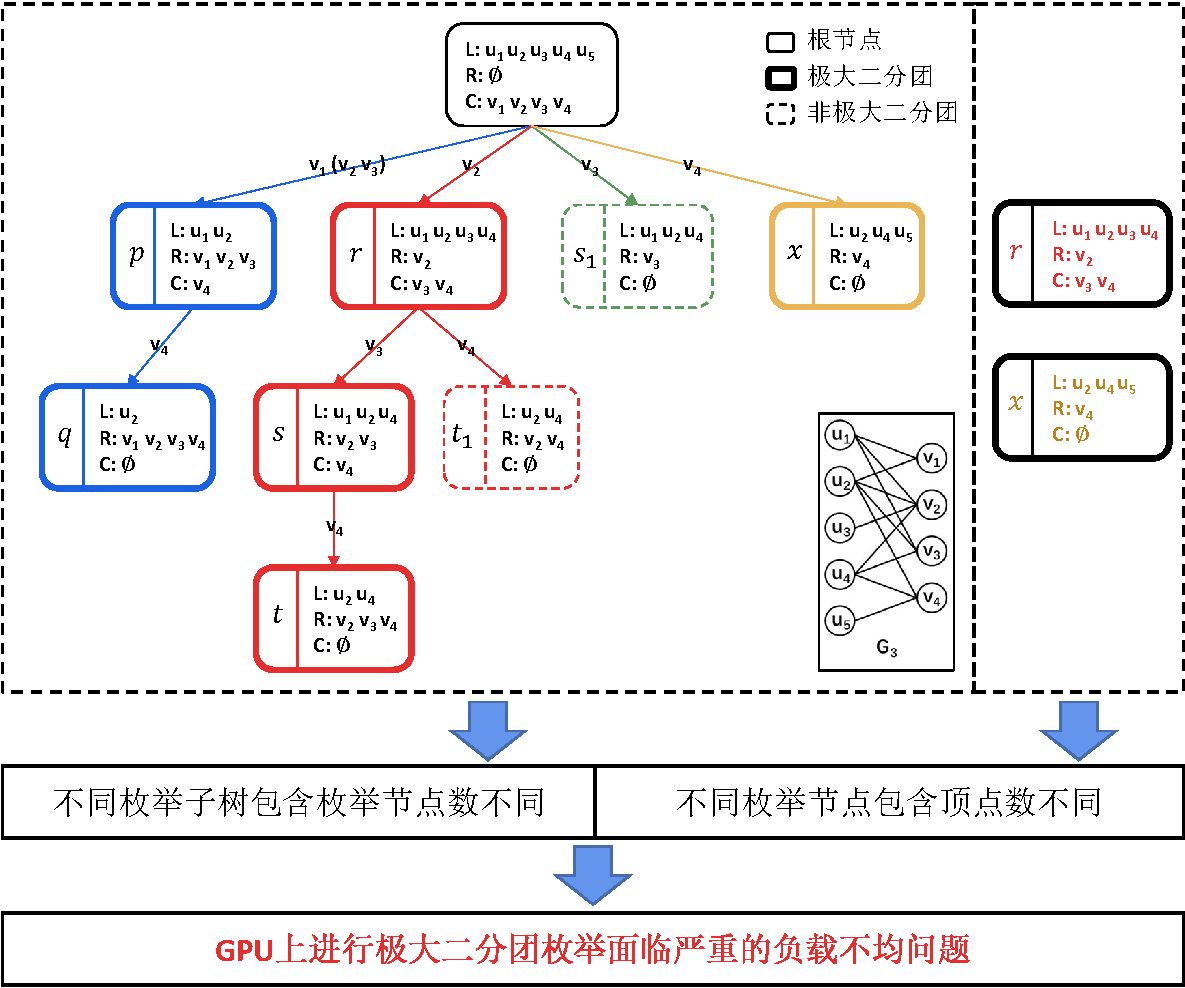
\includegraphics[width=0.85\linewidth]{gmbe/motivation_load}
    \vspace{0.1in}
	\caption{在GPU上进行极大二分团枚举中的负载不均问题说明}
	\label{fig:gmbe_load_reason}
\end{figure}


\subsection{负载不均}

如图~\ref{fig:gmbe_load_reason}所示,极大二分团枚举问题在GPU上面临严重的负载不均问题,这是由于\emph{不同子枚举树和枚举节点之间的计算差异性}所导致的。与其他GPU实现的图挖掘算法类似,我们将完整枚举树拆分成多个子枚举树,并尝试在不同计算单元之间平衡它们的负载分布~\cite{g2miner22,Kclique22,Graphset23}。我们没有选择按照更细粒度的枚举节点进行任务划分,因为在此类图挖掘问题中,枚举节点往往数量庞大,细粒度划分会增加任务调度的开销,严重降低整体性能。
目前,已有的图模式挖掘算法G$^2$Miner~\cite{g2miner22}通常将每个顶点生成的枚举子树分配给GPU上的一个线程束来独立执行。然而,我们的实验结果显示,这种粗粒度的GPU负载均衡策略在极大二分团枚举问题中效率较低。由于不同子枚举树包含的枚举节点数量差异很大,且每个节点内的顶点数量也不同,导致不同子枚举树的负载相差较大。这种负载不均会导致大量计算核心在等待最耗时的核心执行时浪费大量时间,造成资源的浪费。接下来,我们将通过一组实验结果详细说明这一问题。

% 根据图~\ref{fig:gmbe_load_reason}展示的情况,在GPU上运行的极大二分团枚举算法存在严重的负载不均问题,这是由于\emph{不同子枚举树和枚举节点之间的计算差异性}所导致的。负载不均会导致大量计算核心在等待最耗时的计算核心执行时浪费大部分时间,从而造成资源的浪费。目前,已有的图模式挖掘算法G$^2$Miner~\cite{g2miner22}通常将每个枚举子树分配给GPU上的一个线程束来独立执行。


\begin{figure} [H]
  \center
		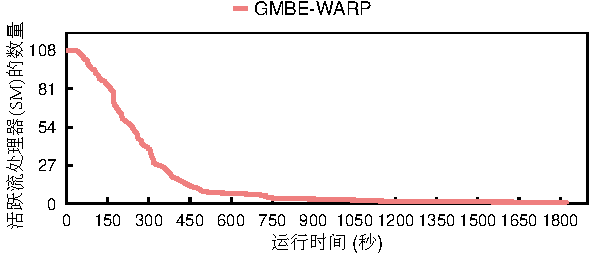
\includegraphics[width=0.7\linewidth]{gmbe/load_balance}
	\caption{在GPU上进行极大二分团枚举的负载不均问题示例}
	\label{fig:gmbe_load_example}
\end{figure}

\begin{example}

  图~\ref{fig:gmbe_load_example}展示了在简单负载均衡方案下,在GPU上进行极大二分团枚举表现出的负载不均问题。具体而言,首先,在我们的最终解决方案GMBE的基础上,我们应用G$^2$Miner算法中将每个顶点生成的枚举子树分配给GPU上的一个线程束来独立执行的任务调度方案,形成变种GMBE-WARP。随后,我们在BookCrossing数据集上运行GMBE-WARP,并记录了GPU内活跃流处理器数量随着运行时间的变化图。实验结果显示,该算法的总运行时间为1,822秒。当程序运行至20\%时(即364秒),活跃的流处理器仅有22个,占总数108个的20\%。这意味着在整个运行过程中,超过80\%的流处理器(86个SMs / 共108个SMs)将耗费80\%的运行时间(1,458秒 / 共1,822秒)等待最慢的一个子枚举树的计算。因此,现有的方法不能满足极大二分团枚举算法在GPU上的负载均衡需要,我们有必要实现更细粒度的负载均衡。
  
\end{example}


% 然而,如图~\ref{fig:gmbe_load_example}所示,如果简单采用我们提出的GMBE算法,将每个枚举树分配给一个线程束,将会导致大量资源浪费,影响性能。具体来说,该算法总共运行时间为1,822秒。当程序运行至20\%时(即364秒),活跃的流处理器仅有22个,占总数108个的20\%。这意味着在整个运行过程中,超过80\%的流处理器(86个SMs / 共108个SMs)将耗费80\%的运行时间(1,458秒 / 共1,822秒)等待最慢的一个子枚举树的计算。因此,对于MBE算法,有必要在更细粒度上平衡工作负载。


\section{GMBE算法}
为了应对GPU上高效实现极大二分团枚举时所面临的内存短缺、线程分歧以及负载不均等挑战,本节提出了一系列对应的解决方案。这些解决方案包括基于枚举节点重用的迭代方法、局部邻居数量感知的剪枝方法以及负载感知的任务调度方法。最终,通过结合这些技术,我们提出了高效的GPU极大二分团枚举算法 GMBE。


\subsection{基于枚举节点重用的迭代方法}
\label{subsec:gmbe_memory}


为了减少内存使用,我们提出了一种基于枚举节点重用的迭代方法。该方法的核心思想在于仅保存子枚举树中的根节点$x$及其相关元数据,\textbf{在迭代过程中反复重用节点$x$的存储空间,避免为大量子节点动态分配空间}。在枚举过程中,后继节点总是能够从节点$x$的存储空间中获取,因为我们发现任何子节点$c$中的顶点集$L_c \cup R_c \cup C_c$始终是其父节点$x$的顶点集$L_x\cup R_x\cup C_x$的子集。例如,在图~\ref{fig:gmbe_tree}中,对于父节点$p$和子节点$q$,我们发现父节点$p$内的顶点集$\{u_1, u_2, v_1, v_2, v_3, v_4\}$包含子节点$q$内的顶点集$\{u_2, v_1, v_2, v_3, v_4\}$,这种父子节点间顶点集间普遍存在的包含关系为枚举节点重用技术提供了理论保证。接下来,我们在图~\ref{fig:gmbe_node_buf}中给出了基本的根节点存储结构,并结合算法~\ref{alg:gmbe_stack}详细描述了基于枚举节点重用的迭代方法。



% 在枚举过程中,我们总是能够实现枚举节点重用,因为我们观察到节点$x$的子节点的$L\cup  R\cup C$总是其父节点$x$的$L\cup  R\cup C$的子集。例如,在图~\ref{fig:gmbe_load_example}中,我们可知子节点$q$ $(\{u_2\},\{v_1, v_2, v_3, v_4\}, \emptyset)$ 中的顶点$\{u_1, u_2, v_1, v_2, v_3, v_4\}$ 是其父节点$p$ $(\{u_1, u_2\}, \{v_1, v_2, v_3\},\{v_4\})$ 中顶点的子集。算法~\ref{alg:gmbe_stack}具体描述了基于枚举节点重用的迭代方法。

\begin{figure} [H]
  \center
    % \vspace{-0.1in}
    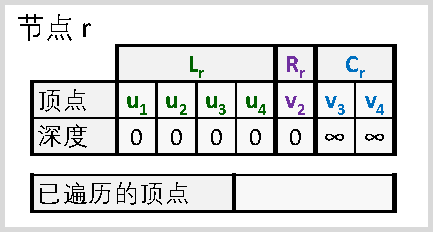
\includegraphics[width=0.4\linewidth]{gmbe/eg_node_buf}
    % \vspace{0.1in}
  \caption{$node\_buf$结构示意图}
  \label{fig:gmbe_node_buf}
\end{figure}


\begin{algorithm} [H]
  \begin{algorithmic}[1]
    \normalsize
    \REQUIRE 二分图 $G(U,V,E)$
    \ENSURE 所有极大二分团
    
    \renewcommand{\algorithmicwhile}{\textbf{procedure}}
    \renewcommand{\algorithmicdo}{\textbf{:}}
    \STATE \textsf{iteratively\_search}$(U,\emptyset,V)$;

    \WHILE{\textsf{iteratively\_search}$(L_r,R_r,C_r)$}
    \renewcommand{\algorithmicwhile}{\textbf{while}}
    \renewcommand{\algorithmicdo}{\textbf{do}}
      \STATE $node\_buf$ \textsf{.init\_and\_push}$((L_r,R_r,C_r))$;
      \WHILE{$node\_buf$非空}
        \STATE $(L_p, R_p, C_p) \leftarrow node\_buf$\textsf{.pop}$()$;
        \IF{$C_p$非空}
          \STATE $v' \leftarrow C_p$ 中编号最小的顶点; 
          \STATE $node\_buf$\textsf{.push}$((L_p,R_p,C_p \setminus \{v'\} ))$;
          \STATE $L' \leftarrow L_p \cap N(v');$ $R'\leftarrow R_p;$ $C' \leftarrow \emptyset$;
          \FOR{$v_c \in C_p$}
            \IF{$L' \cap N(v_c) = L'$}
              \STATE $R' \leftarrow R' \cup \{v_c\}$;
            \ELSIF{$L' \cap N(v_c) \neq \emptyset$}
              \STATE $C' \leftarrow C' \cup \{v_c\}$;
            \ENDIF
          \ENDFOR
          \IF{$R' = \Gamma(L')$}
            \STATE 输出极大二分团$(L', R')$;
            \STATE $node\_buf$\textsf{.push}$((L',R',C'))$;
          \ENDIF
        \ENDIF
        
      \ENDWHILE
    \ENDWHILE

  \end{algorithmic}
  \caption{基于枚举节点重用的极大二分团枚举迭代算法}
  \label{alg:gmbe_stack}
\end{algorithm}


具体而言,我们不再以递归的方式创建和释放枚举节点,而是采用类似栈的结构$node\_buf$进行显式的迭代 。如图~\ref{fig:gmbe_node_buf}所示,每个$node\_buf$包括根节点内的所有顶点、每个顶点的深度属性、以及从根节点到当前节点所遍历的所有顶点。每个\textit{顶点}的\emph{\textit{深度}}根据当前节点的\emph{祖先节点数量}确定。\textit{已遍历的顶点}记录着从子枚举树根节点到当前节点所遍历的顶点,用于回溯搜索。在枚举过程中,我们只需要主动更新\textit{顶点}的\textit{深度}属性以及记录\textit{已遍历的顶点}。通过这种方式,迭代过程可以重用$node\_buf$对应的固定内存区域推导出所有的后继节点,进而极大程度地减少了GPU中的内存开销。算法~\ref{alg:gmbe_stack}首先用根节点初始化$node\_buf$(第3行)。随后算法迭代地获取$node\_buf$中的当前节点$(L_p,R_p,C_p)$(第5行)。如果当前节点的候选顶点非空,则迭代地选择当前节点内其中的一个候选顶点产生新的枚举节点(第6-21行),否则弹出该节点,继续迭代流程。最终,算法与递归算法~\ref{alg:se_mbe}得到相同的计算结果。随后,我们将详细阐述涉及枚举节点重用的关键函数:


\begin{itemize}
  \item  \textsf{init\_and\_push}$((L_r,R_r,C_r))$ : 该函数用于利用子树的根节点$(L_r,R_r,C_r)$创建并初始化$node\_buf$ (第3行)。$node\_buf$存储了$L_r \cup R_r \cup C_r$中的所有顶点,并记录每个顶点的深度以及已遍历的顶点。我们将$L_r \cup R_r$中顶点的深度初始化为0,将$C_r$中顶点的深度初始化为$\infty$。
  
  \item  \textsf{push}$((L',R',C'))$ : 该函数用于向$node\_buf$中压入一个新的子节点$(L',R',C')$ (第8,20行)。首先,根据顶点深度的定义,我们知道当前节点的深度D总是比$node\_buf$中已遍历的顶点多一个。当我们在深度为D处压入一个新节点$(L',R',C')$时,我们知道$L' \subset L_r$, $R' \subset R_r \cup C_r$ 且 $C' \subset C_r$。我们将$L'$内顶点的深度更新为D,$R'$内深度为$\infty$的顶点的深度更新为D。因此,通过访问顶点的深度属性,我们总是能够在原始的$(L_r,R_r,C_r)$对应的$node\_buf$中找到新节点$(L',R',C')$,其中$L'$包含$L_r$内所有深度为D的顶点,$R'$包含$R_r\cup C_r$中所有深度不大于D的顶点,$C'$包含$C_r$中深度为$\infty$的顶点。最后,我们将用于生成节点$(L',R',C')$的已遍历顶点加入到已遍历的顶点集中。

  \item  \textsf{pop}$()$ : 该函数用于得到当前栈顶节点$(L_p,R_p,C_p)$,并利用$node\_buf$回溯到其父节点 (第5行)。当我们在节点深度D处弹出节点$(L_p,R_p,C_p)$时,首先移除已遍历的顶点集中最新遍历的顶点,然后将$L_p$内顶点的深度更新为D-1,将$C_r$内深度为D的顶点的深度更新为$\infty$。
  
\end{itemize}




与传统的单一记录节点内顶点的枚举树节点结构相比,我们提出的$node\_buf$在单个节点上额外记录了顶点\textit{深度}以及\textit{已遍历的顶点},其内存开销的上限为$3 \times \Delta(V) + 2 \times \Delta_2(V)$。但是与传统方法需要动态产生和释放枚举节点不同,$node\_buf$结构能够在枚举过程中被所有后继枚举节点重复使用,因此显著减少了遍历每棵枚举树的内存需求,为在GPU上并发运行数千个极大二分团枚举过程提供可能。例如,一块拥有40 GB内存的A100 GPU足以在BookCrossing数据集上并发运行超过10,000个子枚举树枚举过程,因为每个过程仅需要$(3 \times 13,601 + 2 \times 53,915) \times$ \textbf{sizeof}(int) B = 595 KB。与传统的方法相比,后者需要$13601 \times (13,601 + 53,915)\times$ \textbf{sizeof}(int) B = 3.67 GB,这种枚举节点重用方法在BookCrossing上的内存使用减少了6,178倍。

\subsection{局部邻居数量感知的剪枝方法}
\label{subsec:gmbe_prune}

现有的剪枝方法在GPU上由于线程分歧导致效率较低。为了解决这一问题,我们提出了一种新的剪枝方法,旨在减少枚举空间的同时减少线程分歧。具体而言,参照表~\ref{tab:definition},对于给定节点$(L, R, C)$,我们将顶点$v \in V$的\emph{局部邻居}定义为$N_L(v)$,其中$N_L(v)$等于$N(v) \cap L$。随后,我们定义\emph{局部邻居数量}为局部邻居的顶点个数。在算法~\ref{alg:gmbe_stack}中,候选顶点的局部邻居数量总是作为中间结果出现 (第11、13行),因此,我们能够在不引入额外计算的情况下得到候选顶点的局部邻居数量。基于这一现象,我们总结了如下定理:

\begin{theorem}
  假设当前节点为枚举树中的节点$s$,在选择候选顶点$v_r$时,如果对于当前节点$s$中顶点$v_r$的局部邻居数量与任一子节点$t$中顶点$v_r$的局部邻居数量相等,我们可以安全地裁剪由节点$s$选择顶点$v_r$所产生的子节点。
  \label{theorem:gmbe_prune}
\end{theorem}

\begin{proof}
  为了证明该定理,我们假设节点$s$已经遍历顶点$v_t$产生节点$t$,并且节点$s$将遍历顶点$v_r$产生新的节点$r$。进一步地,我们假设节点$s$中顶点$v_r$的局部邻居数量与子节点$t$中顶点$v_r$的局部邻居数量相等,即$N(v_r) \cap L_s =N(v_r) \cap L_t$。由于$L_t = L_s\cap N(v_t)$,我们知道$N(v_r) \cap L_s =N(v_r) \cap L_t= N(v_r) \cap L_s\cap N(v_t)$,因此$N(v_r) \cap L_s \subseteq N(v_t)$。由于$L_r = N(v_r)\cap L_s$,我们知道$L_r\subseteq N(v_t)$,即$v_t$与$L_r$中的所有顶点相连。由于我们已经遍历$v_t$产生节点$t$,因此节点$r$无法使用$v_t$扩展$R_r$,进而产生非极大二分团。因此我们可以安全地裁剪节点$r$。

\end{proof}

根据定理~\ref{theorem:gmbe_prune},我们观察到可以通过比较父子节点中候选顶点局部邻居数量是否变化进行剪枝。因此,在算法~\ref{alg:gmbe_stack}中,我们通过在$node\_buf$中额外维护所有候选顶点的局部邻居数量来进一步优化。具体而言,在$node\_buf$执行弹出操作\textsf{pop()}弹出节点$r$时,会临时保存栈顶节点候选顶点的局部邻居数量。当恢复到节点$r$的父节点$p$时,我们将对节点$p$和节点$r$中候选顶点的局部邻居数量进行批量比较。如果发现部分候选顶点的局部邻居数量未发生变化,我们可以安全地裁剪这些无用顶点。相比现有剪枝方法中涉及大量判断语句所引入的线程分歧问题,这种剪枝方法在GPU上不会额外引入线程分歧问题,因为剪枝的过程同一线程束中的线程总是批量比较相同候选集中的元素。我们通过一个示例详细展示了基于栈的迭代算法,并利用局部邻居数量进行剪枝。





% 根据定理~\ref{theorem:gmbe_prune},我们观察到可以通过比较父子节点中候选顶点局部邻居数量是否变化进行剪枝。因此,在算法~\ref{alg:gmbe_stack}中,我们通过在$node\_buf$中额外维护所有候选顶点的局部邻居数量来进一步优化。如果在弹出一个已遍历的子节点后,候选顶点的局部邻居数量保持不变,我们便可以裁剪这些无用的候选顶点。这种新的剪枝方法具有较低的线程分歧,因为同一线程束中的线程总是批量比较相同候选集中的元素。我们通过一个示例详细展示了基于栈的迭代算法,并利用局部邻居数量进行剪枝。







\begin{figure} [H]
  \center
    \vspace{0.1in}
		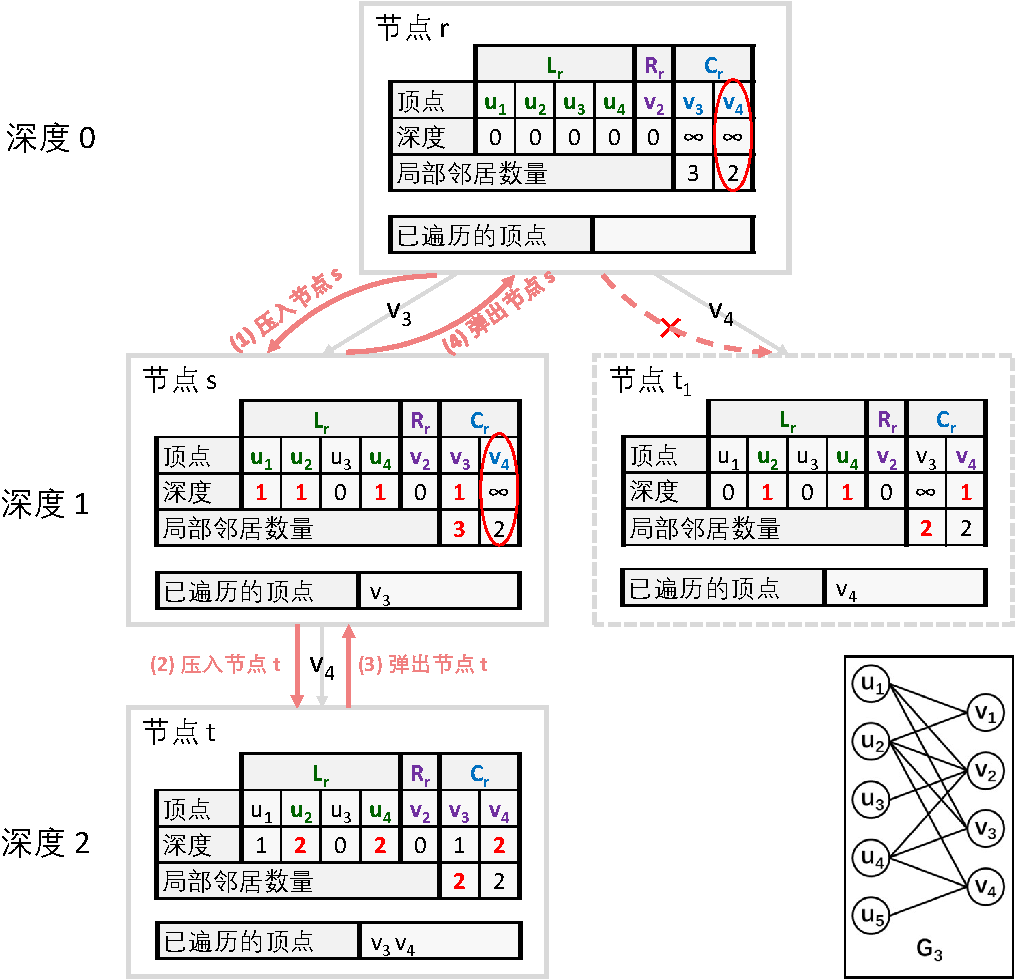
\includegraphics[width=0.8\linewidth]{gmbe/eg_prune}
    \vspace{0.1in}
	\caption{局部邻居数量感知的剪枝方法示意图}
	\label{fig:gmbe_prune}
\end{figure}

\begin{example}
  如图~\ref{fig:gmbe_prune}所示,在图~\ref{fig:gmbe_tree}中以节点$r$为根节点的子树中,算法利用$node\_buf$中固定大小的内存,迭代地枚举了其中的所有极大二分团。具体而言,我们首先使用节点 r $(L_r, R_r, C_r)$初始化$node\_buf$,将$L_r \cup R_r$中的顶点深度初始化为0,并将$C_r$中的顶点深度初始化为$\infty$。对于$C_r$中的顶点,$node\_buf$根据定义初始化了其局部邻居数量(即$|N_L|$)。例如,在节点$r$处,我们初始化$v_3$的局部邻居数量$|N_L(v_3)|$为$|N(v_3) \cap L_r| = 
  |\{u_1, u_2, u_4\}\cap \{u_1,u_2,u_3,u_4\}| = 3$。

  接下来,我们通过遍历$v_3$生成了节点$s$。我们知道$L_s=L_r\cap N(v_3)=\{u_1, u_2, u_4\}$。节点$s$的深度为1,$node\_buf$将$L_s\cup R_s$中顶点$u_1, u_2, u_4,$ 和 $v_3$的深度更新为1。其他顶点的深度保持不变。随后,我们利用$L_s$更新了$v_3$和$v_4$的局部邻居数量。通过计算,我们知道$|N_L(v_3)|$ = $|N(v_3) \cap L_{(s)}|$
  = $|\{u_1, u_2, u_4\} \cap \{u_1, u_2, u_4\}|$ = 3。
  $|N_L(v_4)|$ = $|N(v_4) \cap L_{(s)}|$
  = $|\{u_2, u_4, u_5\} \cap \{u_1, u_2, u_4\}|$ = 2。我们可以类似地生成其他节点。

在处理完以节点$s$为根节点的子树后,$node\_buf$弹出节点$s$并重置顶点的深度和局部邻居数量,用于恢复节点$r$。对于$node\_buf$内深度与节点$s$深度相同的顶点,我们将$u_1$,$u_2$和$u_4$的深度重置为0,并将$v_3$的深度重置为$\infty$。由于弹出节点$s$后,$v_4$的局部邻居数量始终是2,我们主动地在节点$r$处通过移除无用的候选顶点$v_4$来进行剪枝。


\end{example}


\subsection{负载感知的任务调度方法}
\label{subsec:gmbe_design_load}

为了进一步探索极大二分团枚举任务在GPU上的大规模并行性,我们提出了负载感知的任务调度方法。在图挖掘算法的GPU上任务调度方面,一种简单的方法是为每个子枚举树分配一个任务。如算法~\ref{alg:gmbe_task_naive}所示,我们用集合$V$中的不同顶点$v_s$产生不同的枚举子树,分别作为一个任务。

\begin{algorithm} [H]
  \begin{algorithmic}[1]
    \normalsize
    
    \FOR{$v_s \in V$}
      \STATE $L_s \leftarrow N(v_s); R_s\leftarrow\{v_s\}; C_s\leftarrow \emptyset $;
      \FOR{$v_c \in N_2(v_s)$}
        \IF{$L_s \cap N(v_c) = L_s$}
          \STATE $R_s \leftarrow R_s \cup \{v_c\}$;
        \ELSIF{$v_c$的索引在$v_s$之后}
          \STATE $C_s \leftarrow C_s \cup \{v_c\}$;
        \ENDIF 
      \ENDFOR

      \IF{$v_s$是$R_s$中索引最小的顶点}
        \STATE \textsf{iteratively\_search}$(L_s,R_s,C_s)$;
      \ENDIF

    \ENDFOR

  \end{algorithmic}
  \caption{GPU任务调度的简单方法}
  \label{alg:gmbe_task_naive}
\end{algorithm}


然后,我们可以参考已有的图挖掘算法,将每个任务映射到GPU的不同的线程束~\cite{g2miner22}或者不同线程块~\cite{Kclique22}上。我们将两种方案分别称为\textit{基于线程束的调度方法}(Warp-centric Scheme)和\textit{基于线程块的调度方法}(Block-centric Scheme)。然而,我们的研究表明,由于算法~\ref{alg:gmbe_task_naive}在第11行创建的并行任务运行时间差异很大,对于极大二分团问题,这两种简单的调度方法不足以平衡GPU中不同流处理器 (SM)上的任务负载。具体而言,在一个线程束或一个线程块中运行的最慢任务经常阻塞其他任务,导致EuAll数据集上存在97.8\%的性能下降。~\ref{subsec:gmbe_breakdown}节将展示更多任务调度相关的实验结果。




为了更好地平衡GPU中的任务负载,我们提出了一种针对极大二分团枚举的\textit{负载感知的基于任务的调度方法}(Task-centric Scheme)。该方法基于GPU编程模式中的持久线程编程模型(Persistent Thread, PT)~\cite{PersistentThread12}。具体而言,我们根据GPU中的流处理器数量创建对应数量的线程组,将每个线程组固定地映射到一个GPU的流处理器上。随后,为每个线程组设置固定数量的线程束,将每个流处理器上线程束的数量用\textsf{WarpPerSM}表示,并在后文讨论其对系统性能的影响。



我们设计了一个可以创建负载感知任务的GPU核函数(Kernel Function),该函数会将处理较大枚举树的任务递归地分解为更小的任务,并将这些负载感知任务添加到每个流处理器的全局结构\textit{SM\_task\_queue}中。当一个任务完成时,PT的软件调度器会从\textit{SM\_task\_queue}中出队一个任务,并在相应的SM上迭代执行\textsf{}{iteratively\_search()}。

为实现负载感知,关键问题在于高效地检测出哪些负载的任务较重,并及时对高负载任务进行分解。对此,我们根据子枚举树根节点$(L,R,C)$的信息来估计枚举树的高度和节点数量。具体而言,我们估计枚举树的高度为$\min\{|L|,|C|\}$。我们估计枚举树中节点数量为$\min\{|L|,|C|\}\times|C|$,因为$|C|$代表了每个节点能够产生子节点的最大数量。我们经验性地设置了两个阈值$bound\_height$ 和 $bound\_size$,只有当$\min\{|L|,|C|\}$大于$bound\_height$且$\min\{|L|,|C|\}\times|C|$ 大于 $bound\_size$时,我们将该任务分解成多个子任务,以实现更好地负载平衡。

算法~\ref{alg:gmbe_task_full}描述了针对极大二分团枚举问题的GPU负载感知的基于任务的调度算法。当\textit{SM\_task\_queue}不为空时,它从队列里获取一个节点(第6行),如果我们估计该节点对应的负载较小时,我们直接启动一个GPU任务(第37行);反之,如果对应的负载超过阈值时(第23行),我们将该任务拆分成小任务并将小任务对应的根节点入队进行枚举(第23-35行)。这些小任务对应的节点将重新参与\textit{SM\_task\_queue}的调度。如果\textit{SM\_task\_queue}为空时,我们将从$processing\_v$获取需要处理的当前顶点$v_s$。然后用顶点$v_s$产生一个枚举任务,并运行在GPU上(第8-20行)。

\begin{algorithm} [H]
  \begin{algorithmic}[1]
    \normalsize

    \STATE $processing\_v$是一个全局变量,初始化为0;
    \STATE $SM\_task\_queue$是用于负载均衡的全局并发队列 ;
  
    \renewcommand{\algorithmicwhile}{\textbf{procedure}}
    \renewcommand{\algorithmicdo}{\textbf{:}}

    \WHILE{\textsf{warp\_kernel}}
    \renewcommand{\algorithmicwhile}{\textbf{while}}
    \renewcommand{\algorithmicdo}{\textbf{do}}
      \WHILE{\textbf{true}}
        \IF{$SM\_task\_queue$非空}
          \STATE $(L,R,C) \leftarrow SM\_task\_queue$\textsf{.dequeue}$()$ ;
        \ELSE
          \STATE $v_s$ = \textsf{atomicInc}$(processing\_v)$
          \IF{$v_s \in V$}
            \STATE $L \leftarrow N(v_s); R\leftarrow\{v_s\}; C\leftarrow \emptyset $;
            \FOR{$v_c \in N_2(v_s)$}
              \IF{$L\cap N(v_c) = L$}
                \STATE $R \leftarrow R \cup \{v_c\}$;
              \ELSIF{$v_c$的索引在$v_s$之后}
                \STATE $C \leftarrow C \cup \{v_c\}$;
              \ENDIF
            \ENDFOR
          \ELSE
            \STATE \textbf{return};
          \ENDIF
        \ENDIF

        \IF {$R = \Gamma(L)$}
          \IF {$\min\{|L|,|C|\}\times|C| >$ 数量边界,并且$\min\{|L|,|C|\} >$ 高度边界 }
            \FOR{$v_t \in C$}
              \STATE $L_t \leftarrow N(v_t); R_t\leftarrow R; C_t\leftarrow \emptyset $;
              \FOR{$v_c \in C$}   
                \IF {$L_t \cap N(v_c) = L_t$}
                  \STATE $R_t \leftarrow R_t \cup \{v_c\}$;
                \ELSIF{$L_t \cap N(v_c)$ 非空}
                  \STATE $C_t \leftarrow C_t \cup \{v_c\}$;
                \ENDIF
              \ENDFOR
              \STATE $SM\_task\_queue$\textsf{.enqueue}$((L_t, R_t, C_t))$
              \STATE $C \leftarrow C \setminus \{v_t\}$\;
            \ENDFOR
          \ELSE
            \STATE \textsf{iteratively\_search}$(L,R,C)$;
          \ENDIF

        \ENDIF
      \ENDWHILE
    \ENDWHILE 

  \end{algorithmic}
  \caption{负载感知的基于任务的调度方法}
  \label{alg:gmbe_task_full}
\end{algorithm}

\subsection{GMBE算法设计}

基于以上所述技术要点,我们提出了基于GPU的高效极大二分团枚举算法GMBE。除了前文提及的主要技术要点之外,接下来将详细描述GMBE算法的具体实现细节。

\textbf{二分图预处理:} 我们将输入的二分图$G$以压缩稀疏行(Compressed Sparse Row,CSR)格式进行表示。首先将图$G$载入 CPU 内存,并快速提取图$G$ 的重要特征,如$|U|$, $|V|$, $|E|$, 
$\Delta(V)$, 和 $\Delta_2(V)$。由于二分图中$U$和$V$是对称的,在本文中我们总是选择顶点数较少的集合作为$V$,类似于ooMBEA~\cite{ooMBE22}。然后,我们通过按照顶点邻居数量递增的顺序对$V$中的所有顶点进行排序,类似于MineLMBC~\cite{minel06}和iMBEA~\cite{iMBEA14},并对每个顶点的所有邻居列表按照顶点 ID 递增的顺序进行排序,类似于大多数相关工作~\cite{g2miner22,Kclique22}。最后,我们将整个二分图$G$传输到 GPU 的全局内存,并在 GPU 上枚举所有极大二分团,而无需从主机传输任何额外数据。

\textbf{无锁任务队列:} 为了减少同步开销,我们使用 CUDA 中的 \textsf{atomicCAS} 原语以无锁方式管理任务队列。我们实现了一个两级任务排队机制以进一步改善负载平衡。具体来说,我们为每个线程块实现了一个局部任务队列,以便线程块中的所有线程束可以通过访问局部任务队列来平衡工作负载。此外,我们实现了一个全局任务队列来平衡不同线程块之间的工作负载。每个线程块只允许一个代理线程束来管理局部任务队列和全局任务队列之间的任务。我们使用共享内存实现局部任务队列,并在全局内存中实现全局任务队列,因为共享内存上的原子操作比全局内存上的原子操作更快。

\textbf{基于相交路径的集合并集操作:} 为了降低算法~\ref{alg:gmbe_task_full} 第11行计算2跳邻居的开销,我们在GPU上实现了基于相交路径的集合并集操作。这一方法受到了文献~\cite{GpuMergePathIntersect14} 的启发。具体而言,为了并行化集合并集操作,每个线程使用滑动窗口遍历一个相交路径,并在当前窗口内独立查找部分相交路径。最后,线程束中的所有线程同步部分结果,生成完整的相交路径。

\textbf{多GPU上的GMBE算法实现:}高性能计算机可能由多个 GPU 组成,以加速应用执行性能。为了支持这种情况,我们可以轻松地将 GMBE 算法扩展到多 GPU 计算机。其基本思想是在所有 GPU 设备上共享算法~\ref{alg:gmbe_task_full} 中的全局变量$processing\_v$,并将第8行中的\textsf{atomicInc} 原语替换为 \textsf{atomicInc\_system}~\cite{CUDAProgrammingGuide}。因此,MBE 问题被划分为多个独立的子问题,并每个 GPU 独立处理这些子问题。整体运行时间由运行时间最长的 GPU 决定。实验结果显示,GMBE 在多个 GPU 上是高效的,因为多个 GPU 上的每个线程束可以使用原子原语自动平衡工作负载,几乎没有同步开销。从理论上讲,GMBE 也可以扩展到分布式计算环境,其中多台机器(每台机器都有一个或多个 GPU)通过网络连接。由于本文侧重于单机环境,我们将探索将 GMBE 应用于分布式多机集群作为未来工作。


\section{实验评估}
本节将利用真实数据集,通过对比现有的串行和并行方法,全面评估GMBE算法的性能表现。首先,介绍实验环境设置,包括实验平台、数据集、比较对象和测试方法。随后,通过对已有算法在真实数据上的执行情况进行分析,从运行时间的角度对GMBE进行整体评估。接着,通过消融实验,对本章提出的枚举节点重用技术、剪枝技术和负载均衡技术进行详细评估。最后,对涉及的参数、GMBE在不同GPU上的适用性以及在多GPU上的可扩展性进行敏感性测试。

\subsection{实验设置}

\textbf{实验环境设置:} 本节的主要实验在一台配备有1个NVIDIA A100 GPU~\cite{NVIDIA-A100}和4个Intel Xeon(R) Gold 5318Y 2.10GHz CPU 的Linux服务器上进行。其中每个NVIDIA A100 GPU 包括108 个流多处理器(SMs)和 40 GB 全局内存,每个 Intel Xeon(R) Gold 5318Y 2.10GHz CPU 拥有24个计算核心,总计96个计算核心。操作系统为 Linux 内核-5.4.0。在默认情况下,GMBE算法及相关变种在单个A100 GPU上执行,其他现有的基于CPU的比较算法均在CPU上执行。

\begin{table*}[t]
  \setlength{\abovecaptionskip}{0cm}  
  \setlength{\belowcaptionskip}{-0.1cm}
	\centering
	\caption{GMBE实验数据集统计信息}
	\label{tbl:gmbe_datasets}
	\begin{center}
    \setlength{\tabcolsep}{3pt}
		\small
    {
			\begin{tabular}{ccccccccc}
				\hline
          \textbf{数据集} &$\textbf{$\lvert U\rvert$}$ &$\textbf{$\lvert V\rvert$}$&$\textbf{$\lvert E\rvert$}$ &$\textbf{$\Delta (U)$}$ &$\textbf{$\Delta_2 (U)$}$ &$\textbf{$\Delta (V)$}$ &$\textbf{$\Delta_2 (V)$}$ &\textbf{极大二分团数量}\\ \hline

          MovieLens (Mti)	&16,528	&7,601	&71,154	&640	&5,817	&146	&3,217	&140,266\\
          Amazon (WA)	&265,934	&264,148	&925,873	&168	&635	&546	&903	&461,274\\
          Teams (TM)	&901,130	&34,461	&1,366,466	&17	&18,516	&2,671	&2,838	&517,943\\
          ActorMovies (AM)	&383,640	&127,823	&1,470,404	&646	&3,956	&294	&7,798	&1,075,444\\
          Wikipedia (WC)	&1,853,493	&182,947	&3,795,796	&54	&47,190	&11,593	&4,629	&1,677,522\\
          YouTube (YG)	&94,238	&30,087	&293,360	&1,035	&37,513	&7,591	&7,356	&1,826,587\\
          StackOverflow (SO)	&545,195	&96,680	&1,301,942	&4,917	&146,089	&6,119	&31,636	&3,320,824\\
          DBLP (Pa)	&5,624,219	&1,953,085	&12,282,059	&287	&7,519	&1,386	&2,119	&4,899,032\\  
          IMDB (IM)	&896,302	&303,617	&3,782,463	&1,590	&15,451	&1,334	&15,233	&5,160,061\\
          EuAll (EE)	&225,409	&74,661	&420,046	&930	&135,045	&7,631	&23,844	&12,306,755\\
          BookCrossing (BX)	&340,523	&105,278	&1,149,739	&2,502	&151,645	&13,601	&53,915	&54,458,953\\
          Github (GH)	&120,867	&59,519	&440,237	&3,675	&29,649	&884	&15,994	&55,346,398\\
        
        \hline
      \end{tabular}
		}
	\end{center}
  
\end{table*}


\textbf{数据集:} 本节使用 12 个真实世界数据集来验证 GMBE的性能,如表~\ref{tbl:gmbe_datasets} 所示。对于允许两个顶点之间存在多条边的数据集,例如 MovieLens(Mti),我们仅保留每对顶点之间的一个唯一边用于极大二分团枚举分析。这些唯一边的数量用 $|E|$表示。由于在二分图中$U$和$V$是对称的,我们总是将顶点集合中拥有较少顶点的集合设置为$V$,即$|U|>|V|$。我们记录了顶点集的最大度数以及最大二跳度数,用于分析GMBE在特定数据集上的内存使用。我们从 SNAP 仓库~\cite{snapnets} 获取 Amazon 和 EuAll 数据集,并从 KONECT 仓库~\cite{konect} 获取其他数据集。由于极大二分团枚举算法的运行时间主要取决于数据集的极大二分团数量,我们将所有数据集按其极大二分团计数的升序排序。%在后续章节中,我们将大于两百万个极大二分团的数据集称为大数据集。

\textbf{比较算法:} 由于目前没有现有的极大二分团枚举算法能在 GPU 上运行,我们将GMBE与面向 CPU 的极大二分团枚举算法进行比较,包括最近的串行版本,即 MBEA~\cite{iMBEA14}、iMBEA~\cite{iMBEA14}、PMBE~\cite{PMBE20} 和ooMBEA~\cite{ooMBE22},以及最前沿的并行极大二分团枚举算法ParMBE~\cite{parMBE19}。为了公平比较,我们从作者处获取所有竞争对手的经过优化的代码,并在相同平台上运行它们。由于我们的服务器中仅有96个CPU计算核心,我们将ParMBE 设置为 96 个线程运行。

\textbf{测量方法:} 我们测量每个算法的运行时间,不包括从磁盘读取图所花费的时间。在没有特别说明的情况下,GMBE使用枚举节点重用迭代枚举所有极大二分团,通过局部邻居数量裁剪无用节点,并应用负载感知的任务中心方案以实现负载平衡。默认情况下,GMBE将 $bound\_height$ 和 $bound\_size$的阈值分别设置为 20 和 1,500,将 \textsf{WarpPerSM} 设置为 16,并在枚举前根据顶点度按升序对$V$中顶点进行排序。我们还实现了其他变体来评估本文提出的技术,并将在相应的实验中详细介绍这些变体。


\subsection{整体评估}

\begin{table} [t]
	\centering    
	\setlength{\abovecaptionskip}{0cm}  
  \setlength{\belowcaptionskip}{-0.1cm}
	\caption{GMBE 整体运行时间评估(单位:秒)}      
	\label{tbl:gmbe_time}
	\setlength{\tabcolsep}{5pt}
	\begin{center}
				\normalsize{
		\begin{tabular}{cccccccc}
			\hline 

      \textbf{数据集} & \textbf{GMBE} & \textbf{MBEA} & \textbf{iMBEA} & \textbf{PMBE} & \textbf{ooMBEA} & \textbf{ParMBE} & \textbf{加速比} \\ \hline
      Mti & \textbf{0.075} & 14.983 & 5.528 & 6.505 & \uline{2.432} & 2.555 & 32.6 \\
      WA & \textbf{0.009} & 0.838 & 1.055 & 0.922 & 1.412 & \uline{0.536} & 62.8 \\
      TM & \textbf{0.107} & 87.377 & 18.930 & 68.180 & 4.087 & \uline{0.949} & 8.9 \\
      AM & \textbf{0.190} & 131.873 & 39.050 & 887.641 & \uline{11.796} & 13.436 & 62.0 \\
      WC & \textbf{0.630} & 117.220 & 29.828 & 1143.291 & 12.896 & \uline{2.225} & 3.5 \\
      YG & \textbf{0.814} & 1214.139 & 314.321 & 141.712 & 112.834 & \uline{9.439} & 11.6 \\
      SO & \textbf{25} & 10814 & 4533 & 10755 & 758 & \uline{691} & 27.2 \\
      Pa & \textbf{0.11} & 46.72 & 18.66 & 53944.64 & 19.48 & \uline{7.14} & 63.7 \\
      IM & \textbf{2} & 953 & 420 & 9018 & 147 & \uline{123} & 69.8 \\
      EE & \textbf{13} & 7105 & 2386 & 2370 & 1255 & \uline{396} & 30.8 \\
      BX & \textbf{50} & 74471 & 32040 & 9184 & 8367 & \uline{892} & 17.8 \\
      GH & \textbf{132} & 58199 & 30800 & 7321 & 8525 & \uline{2412} & 18.2 \\
      \hline
      
		\end{tabular}
				}
	\end{center}

\end{table}


表~\ref{tbl:gmbe_time} 展示了 GMBE 在真实数据集上与最先进的极大二分团枚举算法的运行时间对比结果。实验结果表明,由于 GMBE 能够高效利用 GPU 上的大量计算资源,因此在所有测试数据集上,GMBE 在 CPU 上比任何其他竞争对手快 3.5倍--69.8倍。具体而言,在单个 A100 GPU 上,GMBE 在 ActorMovies 数据集上的表现超过了 96 核 CPU 上最先进的并行极大二分团枚举算法 ParMBE 达到 70.6倍。与所有在 Github 上花费超过 40 分钟枚举所有极大二分团的现有极大二分团枚举算法相比,GMBE 仅需 132 秒,因此对实际大数据集上的极大二分团枚举是非常有帮助的。此外,我们使用 NVIDIA Nsight Compute 软件~\cite{Nsight} 对 GMBE 进行性能分析。分析结果显示,所有真实数据集上的平均 线程束 执行效率为 64\%,内存利用率为 12\%。这些结果可以归因于极大二分团枚举问题中固有的不规则性~\cite{Irregularity12}。

% \begin{figure} [t]
%   \center
%     \vspace{0.15in}
% 		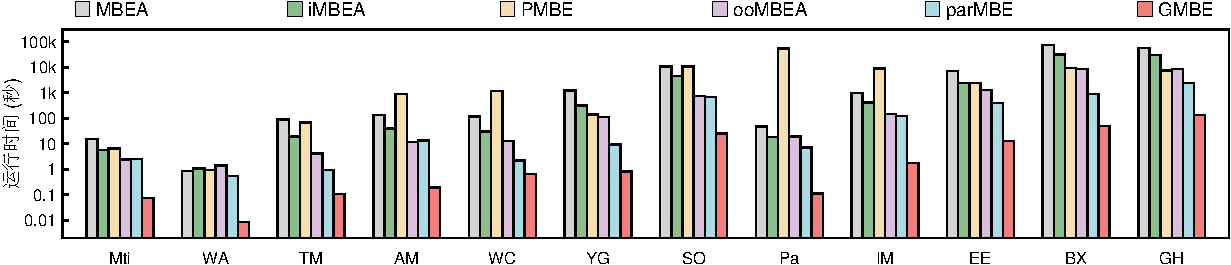
\includegraphics[width=\linewidth]{gmbe/overall}
%     % \vspace{0.05in}
% 	\caption{GMBE整体运行时间评估(对数形式)}
% 	\label{fig:gmbe_exp_overall}
% \end{figure}





\subsection{技术点分解评估}
\label{subsec:gmbe_breakdown}

我们设计了消融实验,分别对GMBE中的枚举节点重用方法、剪枝方法和调度方法等技术点进行了分解评估。

\begin{figure} [H]
	\centering
  \vspace{0.05in}
	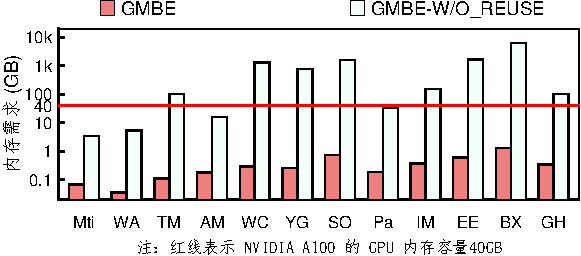
\includegraphics[width=0.75\linewidth]{gmbe/memory.pdf}	
	\vspace{0.05in}
  \caption{枚举节点重用方法的分解评估(对数形式)}
	\label{fig:gmbe_exp_memory}
\end{figure}



\textbf{枚举节点重用方法的效果:} 为了研究~\ref{subsec:gmbe_memory} 节中枚举节点重用方法的效果,我们设计了变体 GMBE-w/o\_REUSE,根据~\ref{subsec:gmbe_memory} 节的要求在 GPU 上预先分配内存。我们分别估计了 GMBE 在是否开启枚举节点重用优化方法的情况下使用 \textsf{cudaMalloc} 原语分配的内存需求。这些内存需求包括用于输入二分图和运行时子树的预分配内存。图~\ref{fig:gmbe_exp_memory} 显示,枚举节点重用方法在所有测试数据集上将内存需求显著减少了 49倍--4,819倍。而 GMBE-w/o\_REUSE 在多个数据集上内存需求超出了 A100 GPU 的内存容量上限,因此导致程序无法运行。




\begin{figure}[t]
	\centering
  \vspace{0.15in}
	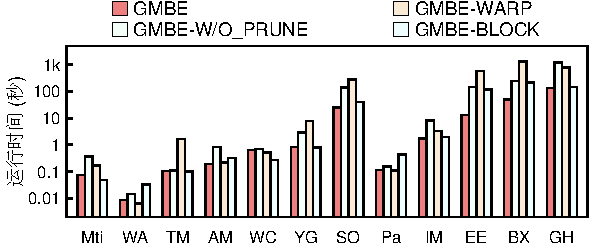
\includegraphics[width=0.75\linewidth]{gmbe/optimization.pdf}	
	% \vspace{0.05in}
  \caption{剪枝方法和任务调度方法的分解评估(对数形式)}
	\label{fig:gmbe_exp_optimization}
\end{figure}

\begin{table}[t]
  % \setlength{\abovecaptionskip}{0cm}  
  \setlength{\belowcaptionskip}{-0.2cm}
	\centering
	\caption{ 剪枝方法使用前后生成的非极大二分团与极大二分团比值比较$\delta/\alpha$}
	\label{tbl:gmbe_prune}
	\begin{center}
    \setlength{\tabcolsep}{3pt}
		\normalsize
    {
			\begin{tabular}{ccccccccccccc}
				\hline
        \textbf{数据集} &Mti &WA &TM &AM &WC &YG &SO &Pa &IM &EE &BX &GH \\ \hline
        GMBE &9.04 &0.734 &1.63 &12.9 &0.71 &2.11 &89.4 &0.362 &15.5 &4.04 &3.40 &11.1 \\ 
        GMBE-w/o\_PRUNE &66.0 &3.68 &3.88 &53.0 &2.89 &20.1 &174 &1.43 &74.4 &56.0 &27.3 &51.4 \\ \hline
        % \hline
        % \textbf{数据集} &Mti &WA &TM &AM &WC &YG  \\ \hline
        % GMBE &9.04 &0.734 &1.63 &12.9 &0.71 &2.11  \\ 
        % GMBE-w/o\_PRUNE &66.0 &3.68 &3.88 &53.0 &2.89 &20.1  \\ \hline \hline
        
        % \textbf{数据集} &SO &Pa &IM &EE &BX &GH \\ \hline
        % GMBE &89.4 &0.362 &15.5 &4.04 &3.40 &11.1 \\ 
        % GMBE-w/o\_PRUNE &174 &1.43 &74.4 &56.0 &27.3 &51.4 \\ \hline

      \end{tabular}
		}
	\end{center}
  \vspace{-0.1in}
\end{table}

\textbf{剪枝方法的效果:} 为了研究~\ref{subsec:gmbe_thread_divergence} 节中局部邻居数量感知的剪枝方法的效果,我们设计了一个变体 GMBE-w/o\_PRUNE,仅禁用了 GMBE 的剪枝功能。如图~\ref{fig:gmbe_exp_optimization} 所示,GMBE 总是优于 GMBE-w/o\_PRUNE。这是因为局部邻居数量感知的剪枝方法通过批量比较局部邻居,在控制线程分歧的同时裁剪了大量极大二分团枚举问题的搜索空间。同时,剪枝方法通过比较候选顶点集中相同顶点的局部邻居数量来增强内存访问的连续性。
为了进一步探索剪枝的效率,我们使用$\alpha$表示极大二分团的数量,使用$\delta$表示通过节点检查(算法~\ref{alg:gmbe_stack} 的第18行)生成的被剪枝的非极大二分团的数量。由于$\alpha$对于每个数据集都保持不变,我们使用比值$\delta/\alpha$来表示 GMBE 和 GMBE-w/o\_PRUNE 的剪枝效率,如表~\ref{tbl:gmbe_prune} 所示。
通过比较 GMBE 和 GMBE-w/o\_PRUNE 的$\delta/\alpha$比值,我们观察到所提出的剪枝方法可以在所有测试数据集中避免 48.7\%-92.8\% 的非极大二分团检查。由于极大二分团枚举任务的枚举空间随着极大二分团数量的增加而增长,剪枝技术在更大的数据集中尤为重要。具体而言,局部邻居数量感知的剪枝方法将运行时间从 Github 上的 1,191 秒显著减少到 132 秒。

\textbf{负载感知的任务调度方法的效果:} 为研究~\ref{subsec:gmbe_design_load}节中负载感知的任务调度方法的效果,我们设计了两个变体 GMBE-WARP 和 GMBE-BLOCK,分别采用基于线程束和基于线程块的方案。如图~\ref{fig:gmbe_exp_optimization}所示,在包括 EuALL、Github、BookCrossing、StackOverflow 和 IMDB 在内的大规模实验数据集上,GMBE明显比 GMBE-WARP 和 GMBE-BLOCK 更快,并在其他数据集上花费不到一秒的时间。在大规模实验数据集上,GMBE 的性能更好,因为它动态检测和分区具有重负载的任务,并管理无锁任务队列以在更细粒度上重新平衡工作负载。实验结果显示,在EuALL数据集上,GMBE、GMBE-WARP和GMBE-BLOCK的运行时间分别为13秒、573秒和119秒。由此可见,相较于其他任务调度方法,负载感知的任务调度方法能够显著提升计算性能,尤其在负载不均匀的情况下表现更为突出。
% 结果,GMBE 在 EuAll 上比 GMBE-WARP 快 44.7倍,比 GMBE-BLOCK 快 9.3倍。

\begin{figure} [H]
	\centering
  \subfloat[StackOverflow]	{
		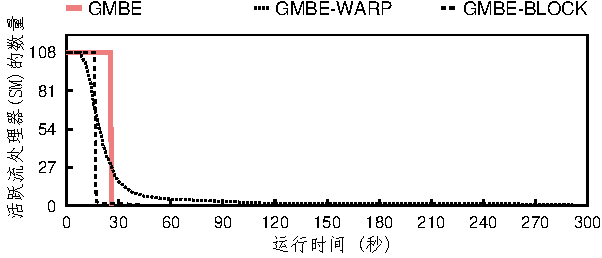
\includegraphics[width=0.47\linewidth]{gmbe/load_balance_so.pdf}
		\label{fig:balance_stackoverflow}
	} 
	\subfloat[EuAll]{
		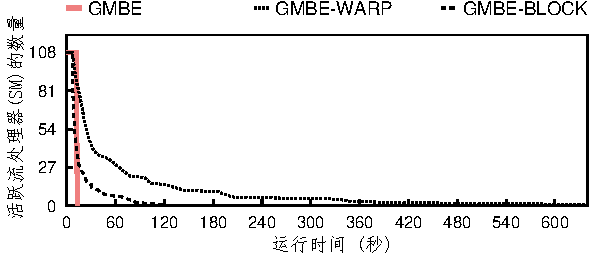
\includegraphics[width=0.47\linewidth]{gmbe/load_balance_ea.pdf}
		\label{fig:balance_euall}
	} \\
	\subfloat[BookCrossing]	{
		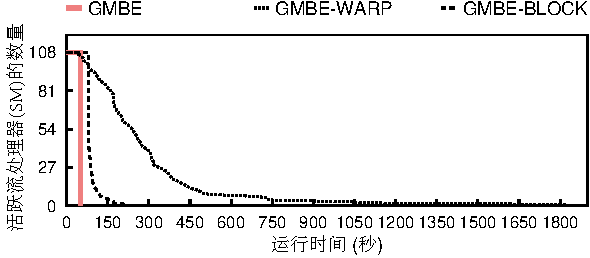
\includegraphics[width=0.47\linewidth]{gmbe/load_balance_bx.pdf}
		\label{fig:balance_bookcrossing}
	}	
  \subfloat[Github]	{
		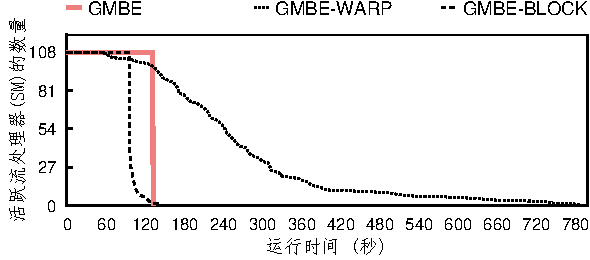
\includegraphics[width=0.47\linewidth]{gmbe/load_balance_gh.pdf}
		\label{fig:balance_github}
	}

	\caption{不同调度方法中SM上的运行时负载比较}

	\label{fig:gmbe_exp_balance}
\end{figure}



为了更深入地探究 GPU 上进行极大二分团枚举 面临的负载不平衡问题,我们记录了在运行 GMBE、GMBE-WARP 和 GMBE-BLOCK 时GPU内活跃流处理器数量随着运行时间的变化情况。图~\ref{fig:gmbe_exp_balance} 对比展示了在StackOverflow、EuALL、BookCrossing 和 Github 数据集上 SM 的运行负载。由于存在工作负载不平衡,一些负载较轻的 SM 可能会提前完成并等待那些负载较重的 SM,这将增加整体运行时间。由于负载不平衡问题的存在,GMBE-WARP 中活跃的 SM 数量迅速减少,因而表现最差。相比之下,GMBE-BLOCK 获得了更好的性能,因为它可以为每个工作负载分配更多资源(即一个线程块而非一个线程束),从而减少了等待具有最重负载的 SM 的时间。然而,GMBE-BLOCK仍然存在不足,因为极大二分团枚举问题的工作负载可能严重不平衡。例如,在 EuALL 数据集上,超过 80\% 的 SM(86 个 SM / 108 个 SM)浪费了超过 80\% 的运行时间(98 秒 / 118 秒)在等待最慢的 SM。相比之下,GMBE 总是能够实现最佳性能,因为它能够在最细粒度上工作,使得每个 SM 大致同时完成其工作。在 BookCrossing 数据集上,甚至在 GMBE-BLOCK 的活跃 SM 数量开始减少之前,GMBE 就已经完成了运算,因为它在每个 SM 中激活了所有的线程束,而相比之下,GMBE-BLOCK 在运行时可能只使用了每个 SM 中的一小部分线程束。



% 图~\ref{fig:gmbe_load_example}展示了在简单负载均衡方案下,在GPU上进行极大二分团枚举表现出的负载不均问题。具体而言,首先,在我们的最终解决方案GMBE的基础上,我们应用G$^2$Miner算法中将每个顶点生成的枚举子树分配给GPU上的一个线程束来独立执行的任务调度方案,形成变种GMBE-WARP。随后,我们在BookCrossing数据集上运行GMBE-WARP,并记录了GPU内活跃流处理器数量随着运行时间的变化图。实验结果显示,该算法的总运行时间为1,822秒。当程序运行至20\%时(即364秒),活跃的流处理器仅有22个,占总数108个的20\%。这意味着在整个运行过程中,超过80\%的流处理器(86个SMs / 共108个SMs)将耗费80\%的运行时间(1,458秒 / 共1,822秒)等待最慢的一个子枚举树的计算。因此,现有的方法不能满足极大二分团枚举算法在GPU上的负载均衡需要,我们有必要实现更细粒度的负载均衡。



\subsection{敏感性测试}
\label{subsec:gmbe_sensitivity}


\begin{figure} [H]
	\centering
  \vspace{0.1in}
	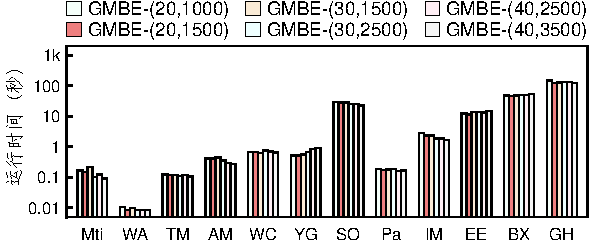
\includegraphics[width=0.8\linewidth]{gmbe/cost_function.pdf}	
	\vspace{0.1in}
  \caption{负载感知任务调度下阈值设置 (对数形式)}
	\label{fig:gmbe_exp_cost}
\end{figure}


\textbf{负载感知任务调度阈值对性能的影响:} 为了探究在~\ref{subsec:gmbe_design_load}节中阈值 $bound\_height$ 和 $bound\_size$ 的有效配置,我们设计了多个变种 GMBE-$(m, n)$,其中$m$ 和 $n$ 分别代表 $bound\_height$ 和 $bound\_size$。我们总是设置 $m$ 大于 $n^2$,因为我们知道  $|L|\times|C|$ 始终大于或等于 $(min\{|L|,|C|\})^2$。阈值的选择是并行粒度和同步开销之间的权衡。我们需要更小的阈值来在更细的粒度上平衡工作负载。然而,阈值不应该过小。否则,我们将不得不处理更多带有巨大同步开销的任务。图~\ref{fig:gmbe_exp_cost} 表明,在大多数情况下,变种 GMBE-(20, 1500) 在运行时间上优于其他变种。因此,GMBE默认应用这种配置。


\begin{figure} [H]
	\centering
  \vspace{0.1in}
	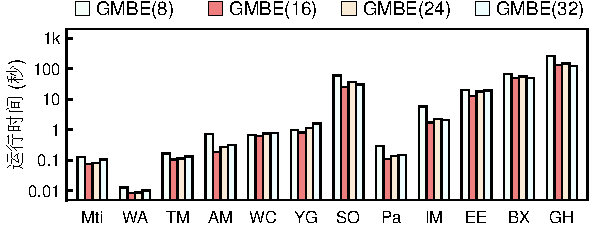
\includegraphics[width=0.8\linewidth]{gmbe/parameters.pdf}	
	\vspace{0.1in}
  \caption{参数\textsf{WarpPerSM}设置 (对数形式)}
	\label{fig:gmbe_exp_config}
\end{figure}

\textbf{每个流处理器中线程束数量的影响:} 为确定~\ref{subsec:gmbe_design_load} 节中 PT 模型中参数 \textsf{WarpPerSM},我们设计了将 \textsf{WarpPerSM} 设置为 8、16、24 和 32 的不同变种。参数\textsf{WarpPerSM} 的选择是并行性和每个线程束资源之间的权衡。直觉上,我们希望 \textsf{WarpPerSM} 更大,以便可以并行运行更多的极大二分团枚举任务。然而,\textsf{WarpPerSM} 不应该过大,因为每个流多处理器中的计算资源(例如寄存器)是有限的。较大的 \textsf{WarpPerSM} 可能会降低 GMBE的性能,因为每个线程束将拥有更少的资源来运行极大二分团枚举任务。图~\ref{fig:gmbe_exp_config} 显示,在大多数大规模数据集(如 BookCrossing、StackOverflow、IMDB、DBLP 和 EuAll)中,变种 GMBE-16的性能优于其他变种 3.83倍。此外,由于其广泛的枚举空间需要更多线程束并行枚举极大二分团,GMBE-16在 Github 上比 GMBE-32慢 0.94倍。考虑到在大多数情况下的效率,GMBE默认将 \textsf{WarpPerSM} 设置为 16。

\begin{figure} [H]
	\centering
	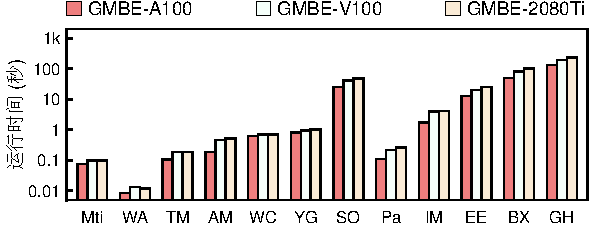
\includegraphics[width=0.8\linewidth]{gmbe/diffgpus.pdf}	
	\vspace{0.1in}
  \caption{GMBE在不同型号GPU上的适用性(对数形式)}
	\label{fig:gmbe_exp_diff}
\end{figure}

\textbf{在不同GPU上的适用性:} 为了探究GMBE在不同GPU上的适用性,我们分别在NVIDIA A100 GPU(108个流多处理器,40 GB全局内存)、NVIDIA V100 GPU(80个流多处理器,32 GB全局内存)~\cite{NVIDIA-V100}和NVIDIA 2080Ti GPU(68个流多处理器,11 GB全局内存)~\cite{NVIDIA-2080Ti}上对GMBE进行评估。图~\ref{fig:gmbe_exp_diff} 显示GMBE在所有三种GPU上都表现出了适用性。GMBE-A100 稍微快于 GMBE-V100 和 GMBE-2080Ti,因为A100 GPU包含比其他GPU更多的计算资源。

\begin{figure} [H]
	\centering

	\subfloat[BookCrossing]	{
		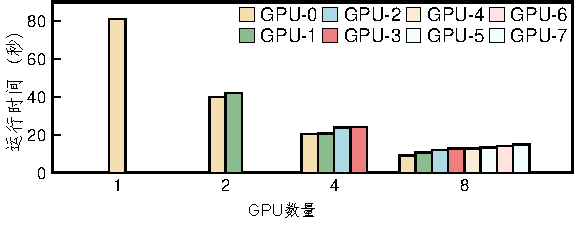
\includegraphics[width=0.8\linewidth]{gmbe/multi_scalability_BookCrossing.pdf}
		\label{fig:scalability_bookcrossing}
	} \\

	\subfloat[Github]	{
		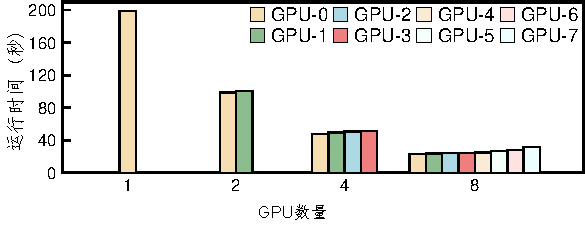
\includegraphics[width=0.8\linewidth]{gmbe/multi_scalability_Github.pdf}
		\label{fig:scalability_github}
	}

	\caption{GMBE在多GPU环境下的可扩展性}

	\label{fig:gmbe_exp_scale}

\end{figure}

\textbf{多GPU环境下的可扩展性:} 为了探究GMBE在多GPU环境下的可扩展性,我们在一台配备了8个NVIDIA V100 GPU的机器上进行了实验。为了优化GMBE以适应多GPU配置,我们将问题分解为多个独立的子问题,总运行时间由运行时间最长的子问题决定。 图~\ref{fig:gmbe_exp_scale} 显示,随着GPU数量的增加,GMBE在Github和BookCrossing数据集上呈线性扩展,因为每个GPU几乎同时完成其执行。在多个GPU的帮助下,GMBE能够在31秒内枚举出Github数据集中超过5500万个极大二分团,相较于96核CPU机器上最先进的并行极大二分团枚举算法ParMBE(即2411秒),性能提升了77倍。

\section{本章小结}

本章介绍了针对极大二分团枚举问题的高效GPU解决方案GMBE。首先,针对GPU上运行极大二分团枚举算法所带来的内存短缺问题,我们提出了基于枚举节点重用的迭代方法,通过重用根节点内存,减小动态内存分配带来的内存开销。其次,针对现有剪枝方法引入的线程分歧问题,本章提出了局部邻居数量感知的剪枝方法,通过对中间结果的批量比较,在实现高效剪枝性能的同时缓解了线程分歧问题。再次,针对现有方法难以实现极大二分团枚举任务负载均衡的问题,本章提出了负载感知的任务调度方法,动态识别并拆分具有高负载的任务,实现细粒度的任务调度。最后,我们结合上述技术,实现了GMBE算法。实验结果充分证明了GMBE算法在GPU上的高性能以及本章中所有方法的具体作用。
\chapter{总结与展望}

本章对全文的研究内容和主要创新点做出总结,并对极大二分团枚举问题的未来可以继续探索的研究问题和方向进行展望。

\section{工作总结}

随着信息技术的迅猛发展,大规模数据的生成和积累已成为常态。为了充分挖掘和利用这些数据中的有效关联信息,二分图结构被广泛应用于表示两个不同群体之间的联系,比如在电子商务场景中用户和商品之间的购买关系。极大二分团是二分图中的一类稠密子图,代表着数据集中那些紧密连接的群体,能够有效揭示二分图中存在的某种规律或共同特征,为探究群体行为内部的脉络和联系提供帮助。极大二分团枚举问题的目标是高效地识别并枚举给定二分图中的全部极大二分团,该问题具有广泛的应用场景,并受到学术界和工业界的广泛关注。本文的主要工作是研究高效的极大二分团枚举方法。针对极大二分团枚举问题中搜索空间庞大、使用静态数据结构以及并行扩展性差等问题,本文从搜索空间剪枝方法、自适应的数据结构和基于GPU的并行实现三个方面分别提出了三种独立的极大二分团枚举方法。通过大量实验证明,这三种方法相较于现有的极大二分团枚举方法均表现出明显的性能优势。本文的主要研究内容和贡献如下:

\textbf{(1)激进的极大二分团枚举剪枝方法:} 为了优化极大二分团枚举问题的搜索空间,现有工作设计了多种优化方法。然而,现有工作的搜索空间仍然非常庞大,在枚举过程中仍然会生成大量的非极大二分团,消除非极大二分团的过程带来高昂的节点检查开销。对此,我们提出了激进的极大二分团枚举算法AMBEA,主要包括激进的集合枚举树(ASE)和激进的顶点合并剪枝方法(AMP)两个核心技术点。激进的集合枚举树打破了现有枚举树仅允许使用部分顶点进行节点生成的结构限制,总是使用全部顶点将每个二分团扩展为极大二分团,裁剪了大量产生非极大二分团的分枝。激进的顶点合并剪枝方法打破了现有剪枝方法由特定顶点触发的限制,通过改变节点的生成过程,主动地合并具有相同局部邻居的顶点,提升剪枝效率。实验结果表明,AMBEA对比最新的ooMBEA等算法压缩了2.37-8.98倍的搜索空间,缩短了1.15-5.32倍的运行时间。

\textbf{(2)自适应的极大二分团枚举数据结构:} 现有的极大二分团枚举问题研究往往注重于算法优化,却忽略了数据结构表示所带来的固有低效性问题,导致现有方法仅适用于小数据集,其中包含不超过1亿个极大二分团。针对这一问题,我们提出了自适应的极大二分团枚举算法AdaMBE,主要包括基于局部计算子图的优化方法(LCG)和基于位图的动态子图方法(BDS)两个核心技术点。为解决现有方法忽略了枚举过程中子图动态变化特性而导致的大量无效内存访问问题,基于局部计算子图的优化方法通过动态缓存枚举过程中的计算子图,优化算法的枚举过程,从而减少无效的顶点访问、集合运算和枚举节点。考虑到现有方法在邻接表上进行大量集合运算会带来高计算开销,基于位图的动态子图方法在枚举过程中动态生成位图,并通过位图上的位运算加速集合运算。该方法充分结合了邻接表与位图两种不同表示方法的优势,同时也考虑到二分图中两个顶点集大小不同的特性。实验结果显示,AdaMBE相比最新的ooMBEA等算法,运行时间缩短了1.6至49.7倍,并成功处理了TVTropes数据集中超过190亿个极大二分团的枚举需求。

\textbf{(3)基于GPU的极大二分团枚举并行实现:}目前,现有的极大二分团枚举算法均采用CPU实现,但其并行扩展性受到CPU计算核心数量的限制。为解决这一问题,我们引入了具有大量计算核心的GPU作为计算资源,用于加速极大二分团枚举过程。我们提出了基于GPU的高效极大二分团枚举解决方案GMBE,主要包括基于枚举节点重用的迭代方法、局部邻居数量感知的剪枝方法以及负载感知的任务调度方法,分别用于解决内存短缺、线程分歧和负载不均等问题。基于枚举节点重用的迭代方法仅存储子枚举树根节点以及对应的元数据,通过重用枚举树根节点的内存,避免为新枚举节点动态分配内存,从而减少内存开销。局部邻居数量感知的剪枝方法通过记录枚举过程中顶点局部邻居数量的变化来对枚举空间进行剪枝,并通过批量比较局部邻居的方法,在剪枝的同时最小化线程分歧问题。负载感知的任务调度方法将每棵子枚举树对应的计算任务与一个线程束的计算资源 
进行绑定,在运行时动态预估子枚举树的大小并对较大的子枚举树进行进一步拆分,实现了细粒度的负载均衡。实验结果显示,基于GPU的GMBE方法比现有基于96个CPU的并行算法ParMBE实现了70.6倍的性能提升。

综上所述,本文聚焦于极大二分团枚举问题。从剪枝方法、数据结构和并行实现三个方面进行探索,提出了三种独立的解决方案和多个通用的核心技术点。这些方法将极大二分团算法的枚举能力提升至百亿级别,并将其实现介质扩展至GPU。

\section{研究展望}

极大二分团枚举问题作为图数据挖掘和图论领域中的经典难题,在广泛应用的同时,与图模式挖掘、极大团枚举等问题密切相关。尽管本文已经就极大二分团枚举问题展开了多方面的探索和实践,但相关领域仍有许多问题值得深入探究和发掘。未来的研究可以在以下几个方面展开:

\textbf{(1)极大二分团枚举问题深度优化:} 首先,从技术路线的宏观层面来看,目前本文提出的三条技术路线相互独立。对枚举性能的深入挖掘可以从融合不同的技术路线入手。例如,可以将AdaMBE中的基于位图的动态子图方法应用于AMBEA或GMBE算法中,结合邻接表和位图两种图表示方法对这两种算法进行进一步的性能优化。其次,从枚举过程中节点计算的中观层面来看,我们研究发现节点检查在枚举过程中占用大量的枚举时间。虽然目前的研究方法已经提出大量的剪枝优化方法,但高开销的节点检查过程仍无法避免。考虑到现有方法都是针对算法本身设计的启发式方法,未来的研究工作可以尝试引入机器学习方法,通过深度网络模型对枚举节点进行快速批量检查,进而优化枚举性能。最后,从集合运算和顶点访问的微观层面来看,虽然AdaMBE方法注意到了计算过程中的细粒度冗余问题,即无效顶点访问问题,但冗余计算仍然大量存在。未来的研究工作可以从冗余的角度进行深入优化,例如从系统层面同时处理多个枚举节点并实时动态减少冗余,进一步提升极大二分团枚举的性能。

\textbf{(2)相关图挖掘问题的深度优化:} 在本文的研究过程中,我们发现极大二分团枚举问题中的技术挑战在相关图挖掘问题中同样存在。这导致目前的极大团枚举问题的GPU实现方案性能不如传统的CPU实现,在图模式挖掘问题中,目标子图内的顶点数量通常较少(不超过10个)。为了解决这一问题,未来的研究工作可以考虑以下几个方面的优化:首先,可以将AMBEA中的剪枝优化方法迁移到相关问题中,以突破相关问题中枚举树的结构限制。通过引入更高效的剪枝策略,可以减少枚举过程中的无效计算,从而提升相关图挖掘问题的性能。其次,可以将AdaMBE中混合不同图表示的思路迁移到相关问题中,加速问题求解过程中大量的集合交集运算。通过选择合适的图表示方法,并结合适当的数据结构和算法设计,可以有效降低集合操作的计算复杂度,从而提高相关图挖掘问题的效率。最后,可以将GMBE中枚举节点重用与任务感知的细粒度任务调度方法迁移到相关问题中,进一步拓展图模式挖掘问题中的目标子图规模。通过合理地利用枚举节点重用技术和任务感知的调度策略,可以优化多任务之间的调度效率,提高相关图挖掘问题的可扩展性和并行性。通过以上的优化措施,我们有望在相关图挖掘问题中实现更高效的算法设计与实现,进而推动相关图挖掘领域的进步。

\textbf{(3)极大二分团枚举问题的应用领域扩展:} 近年来,研究者们在不同类型的二分图上定义了各种形式的二分团,从而拓宽了二分图数据挖掘的研究内容和应用领域。考虑到极大二分团枚举问题在这类挖掘中的基础地位,我们的研究工作将在相关衍生问题中扮演着基础性的角色。例如,在最大边二分团搜索问题中,我们可以基于任一极大二分团枚举算法,并结合现有的最大边二分团搜索问题的剪枝策略,提出新的高效实现方案。同样地,我们的研究成果也可应用于优化类似的二分团枚举问题,如相似二分团枚举、(p,q)二分团枚举、公平极大二分团枚举以及二分团渗透社区等问题的求解。这为未来更多自定义二分团挖掘算法的优化提供了多方面的思路与启示。












% \chapter{关于本模板}

% 本模板根据浙江大学研究生院编写的《浙江大学研究生学位论文编写规则》~\cite{zjugradthesisrules},
% 在原有的 zjuthesis 模板~\cite{zjuthesis}基础上开发而来。

% 本模板的本科生版本\cite{zjuthesisrules}得到了浙江大学本科生院老师的支持与审核,
% 已经在本科生院网上公示。
% 但当前的研究生版本并未经过研究生院老师的审核,
% 同学们使用时要注意对照模板与要求,
% 切不可盲目使用。

% 作者本人并未编写过浙江大学研究生毕业论文,
% 所以不清楚具体要求。
% 如果有热心同学愿意帮忙,
% 可以替我联系相关老师,我会配合审核并修改代码。

% \section{Overleaf 使用注意事项}

% 如果你在Overleaf上编译本模板,请注意如下事项:

% \begin{itemize}
%     \item 删除根目录的 ``.latexmkrc'' 文件,否则编译失败且不报任何错误
%     \item 字体有版权所以本模板不能附带字体,请务必手动上传字体文件,并在各个专业模板下手动指定字体。
%         具体方法参照 GitHub 主页的说明。
%     \item 当前的Overleaf默认使用TexLive 2017进行编译,但一些伪粗体复制乱码的问题需要TexLive 2019版本来解决。
%         所以各位同学可以在Overleaf上编写论文时务必切换到TexLive 2019或更新版本来编译,以免产生查重相关问题。
%         具体说明参照 GitHub 主页。
% \end{itemize}


% \section{节标题}

% 我们可以用includegraphics来插入现有的jpg等格式的图片,
% 如\autoref{fig:zju-logo}所示。

% \begin{figure}[htbp]
%     \centering
%     \includegraphics[width=.3\linewidth]{logo/zju}
%     \caption{\label{fig:zju-logo}浙江大学LOGO}
% \end{figure}


% \subsection{小节标题}


% \par 如\autoref{tab:sample}所示,这是一张自动调节列宽的表格。

% \begin{table}[htbp]
%     \caption{\label{tab:sample}自动调节列宽的表格}
%     \begin{tabularx}{\linewidth}{c|X<{\centering}}
%         \hline
%         第一列 & 第二列 \\ \hline
%         xxx & xxx \\ \hline
%         xxx & xxx \\ \hline
%         xxx & xxx \\ \hline
%     \end{tabularx}
% \end{table}


% \par 如\autoref{equ:sample},这是一个公式

% \begin{equation}
%     \label{equ:sample}
%     A=\overbrace{(a+b+c)+\underbrace{i(d+e+f)}_{\text{虚数}}}^{\text{复数}}
% \end{equation}

% \chapter{另一章}


% \begin{figure}[htbp]
%     \centering
%     \includegraphics[width=.3\linewidth]{example-image-a}
%     \caption{\label{fig:fig-placeholder}图片占位符}
% \end{figure}

% \chapter{再一章}

% \par 如\autoref{alg:sample},这是一个算法

% \begin{algorithm}[H]
%     \begin{algorithmic} % enter the algorithmic environment
%         \REQUIRE $n \geq 0 \vee x \neq 0$
%         \ENSURE $y = x^n$
%         \STATE $y \Leftarrow 1$
%         \IF{$n < 0$}
%             \STATE $X \Leftarrow 1 / x$
%             \STATE $N \Leftarrow -n$
%         \ELSE
%             \STATE $X \Leftarrow x$
%             \STATE $N \Leftarrow n$
%         \ENDIF
%         \WHILE{$N \neq 0$}
%             \IF{$N$ is even}
%                 \STATE $X \Leftarrow X \times X$
%                 \STATE $N \Leftarrow N / 2$
%             \ELSE[$N$ is odd]
%                 \STATE $y \Leftarrow y \times X$
%                 \STATE $N \Leftarrow N - 1$
%             \ENDIF
%         \ENDWHILE
%     \end{algorithmic}
%     \caption{\label{alg:sample}算法样例}
% \end{algorithm}